%% ============================================================
%%  Supporting Information. Tables in si/tab_*.tex are generated by
%%  PaperData/Task4_PhaseTransition/paper_si_tables.py; do not edit them by hand.
%%  Local build: tectonic -X compile SupportingInformation.tex
%% ============================================================
\documentclass[journal=cmatex, manuscript=suppinfo]{achemso}
\usepackage[version=4]{mhchem}
\usepackage{graphicx}
\usepackage{booktabs}
\usepackage{longtable}
\usepackage{pdflscape}
\usepackage{siunitx}
\usepackage{amsmath}
\usepackage{xcolor}
\usepackage[T1]{fontenc}
%% Shared by JCTCmain.tex and SupportingInformation.tex
%% ----- siunitx setup --------------------------------------
\sisetup{
  separate-uncertainty = true,
  range-phrase         = --,
  range-units          = single,
}
%% Declare \angstrom for siunitx v3 (deprecated from built-ins)
\DeclareSIUnit\angstrom{\textup{\AA}}
\DeclareSIUnit\hartree{Ha}
\DeclareSIUnit\bohr{Bohr}

%% ----- Convenience macros ---------------------------------
\newcommand{\CsSnI}{\ce{CsSnI3}}
\newcommand{\MASnI}{\ce{MASnI3}}
\newcommand{\FASnI}{\ce{FASnI3}}
\newcommand{\rSCAN}{r\textsuperscript{2}SCAN}
\newcommand{\Tc}{\ensuremath{T_\mathrm{c}}}
\newcommand{\dTc}{\ensuremath{\Delta T_\mathrm{c}}}
\newcommand{\Eg}{\ensuremath{E_\mathrm{g}}}
\newcommand{\dEg}{\ensuremath{\Delta E_\mathrm{g}}}
\newcommand{\apc}{\ensuremath{a_\mathrm{pc}}}
\newcommand{\todo}[1]{\textcolor{red}{\textbf{[#1]}}}  % draft notes

\newcommand{\TODO}[1]{\todo{#1}}  % alias used in si/configurationGeneration.tex

%% Changes of 2026-10-26 (CsSnI3 band-gap results frozen) in blue for review (user). To print them
%% black, redefine \changedcolor as \relax; blocks use {\changedcolor ...}, inline text \changed{...}.
% 2026-11-12 (user): blue removed, only the orange \placeholder text (PBEsol values) stays coloured
% \newcommand{\changedcolor}{\color{blue}}
\newcommand{\changedcolor}{\relax}
\newcommand{\changed}[1]{{\changedcolor #1}}
% PBEsol numbers standing in for r2SCAN results not yet computed (2026-10-30); remove before submission.
\newcommand{\placeholder}[1]{{\color{orange}#1}}

\graphicspath{{figures/}}
\renewcommand{\thetable}{S\arabic{table}}
\renewcommand{\thefigure}{S\arabic{figure}}
\renewcommand{\thesection}{S\arabic{section}}
\setcounter{secnumdepth}{2}

\author{Kartick Ramakrishnan}
\affiliation[Paramanu Sciences]{Paramanu Sciences, Chennai 600090 India}
\author{Shashikant Kumar}
\affiliation[Ursa Simulation]{Ursa Simulation Inc, Atlanta Georgia USA}
\author{Swarnava Ghosh}
\affiliation[ORNL]{Oak Ridge National Laboratory, Tennessee, USA}
\author{Ray}
\email{ray@ursasimulation.com}
\affiliation[Ursa Simulation]{Ursa Simulation Inc, Atlanta Georgia USA}
% \title{Clamped at the Anneal: How Manufacturing Sets the Operating Band Gap of Tin Halide Perovskites}
\title{\changed{Tin Iodide Perovskites under Processing Strain: Why Tilts Differ, and How They Set Band Gap and Iodide Migration}}

\begin{document}
\maketitle
\tableofcontents

% Body of the Supporting Information: \input by SupportingInformation.tex (standalone) and by
% JCTCmain.tex after the acknowledgement (user 2026-10-15: SI in the main manuscript for now).
% Generated tables: si/tab_*.tex (Task4_PhaseTransition/paper_si_tables.py, PaperData/paper_figs/*.py).
%% ------------------------------------------------------------
% =====================================================================================
% Configuration generation (Task 1): the protocol that produced the pool of candidate structures.
% SOURCES: PaperData/plan-docs/Task1_configuration_generation_plan.md (v1.4+), the generators
% PaperData/code/sampleGen/{common.py,s1..s8,s5supercell}, PaperData/Task1_output/task1_summary.csv,
% PaperLatex/configurationGeneration.tex (earlier version of this text). Rewritten in full sentences 2026-10-15;
% small energies converted to atomic units (1 meV = 36.75 microHa; 0.05 eV/A = 9.7e-4 Ha/Bohr).
% =====================================================================================

\section{Configuration generation and sampling}
\label{sec:configgen}

The training data of the machine-learned force fields are built in three steps: configuration
generation, which is described here, down-sampling in descriptor space, and DFT labelling (main
text, \emph{Identifying structures for DFT labelling}). Configuration generation produces a
deliberately oversampled pool of \num{55928} structures of \CsSnI{}, \MASnI{} and \FASnI{}. The pool
has to span, with margin, every state that the production simulations visit: the $\alpha$, $\beta$
and $\gamma$ perovskite phases and the transitions between them, temperatures from the orthorhombic
phase to above the cubic transition, the lattice strains produced by thermal expansion, by the
spontaneous strain of each transition and by substrate clamping, and disordered orientations of the
molecular cations.

\subsection{Sampling model and molecular-dynamics engine}
\label{sec:configgen:engine}

\paragraph{Sampling model.} The structures are sampled with our in-house foundation model. For
sampling, the neighbour-list capacities in the header of the model file were enlarged from (76, 40)
to (120, 60) neighbours. These numbers size buffers only: energies, forces and stresses are bitwise
identical to those of the original file, but compressed low-temperature hybrid cells need more than
the original radial capacity. The model only proposes plausible structures. Every structure selected
for labelling is recomputed with DFT, so the errors of the sampling model affect where configuration
space is sampled but never the labels.

\paragraph{Rejected alternative.} We first tested a public general-purpose foundation
model\cite{Song2024NEP89} and rejected it. In \SI{50}{ps} constant-volume runs at the experimental
volume it collapsed the \CsSnI{} framework at \SIlist{300;500}{\kelvin} and the \MASnI{} and
\FASnI{} frameworks already at \SI{200}{\kelvin}, producing Sn--Sn distances of
\SI{2.7}{\angstrom} and mean Sn--I coordination numbers of 2.9 to 5.4.

\paragraph{Engine.} All sampling MD uses the batched GPU engine of UrsaMLFF (commit
\texttt{4f4f697e1}). It integrates the equations of motion in double precision and accumulates
forces in 64-bit fixed point, so that a run is bitwise reproducible for a given input and seed, and
it evaluates many independent systems concurrently on one GPU. Two engine defects found during this
work are fixed in that commit and are documented and tested in the engine repository. First,
trajectory frames written during constant-pressure runs carried the cell of the start of the run
segment. Second, in cells thinner than $2.5(r_\mathrm{c}+r_\mathrm{skin})$ the engine uses explicit
periodic-image atoms, and a system that outgrew the image region sized at start-up was integrated
with missing periodic images until the next output frame; atoms are now wrapped into the cell at
every regeneration of the images, and an overflowing system is stopped immediately. All data reported
here were generated after both fixes.

\paragraph{Qualification.} Before sampling we checked the model in three ways. First, along an
isotropic energy--volume scan the pressure obtained from the stress equals $-\mathrm{d}E/\mathrm{d}V$;
the zero-pressure pseudo-cubic lattice constants are \SI{6.29}{\angstrom} for \CsSnI{} and about
\SI{6.40}{\angstrom} and \SI{6.49}{\angstrom} for \MASnI{} and \FASnI{}, 1 to \SI{3}{\percent}
larger than experiment, as expected for a PBE-based model. Second, in constant-volume MD at the
experimental volume the Sn--I framework stays intact from \SIrange{200}{500}{\kelvin} for all three
compounds, with a mean Sn--I coordination of at least 5.9 and no Sn--Sn distance below
\SI{5}{\angstrom}; these runs were repeated with the corrected engine. Third, in flexible
constant-pressure MD at \SI{0}{\giga\pascal}, \CsSnI{} at \SI{500}{\kelvin} and both hybrids at
\SI{300}{\kelvin} expand without bound (pseudo-cubic lattice constants above \SI{7.2}{\angstrom}
for the hybrids) and their frameworks decompose (Sn--Sn distances of about \SI{2.7}{\angstrom}),
because the model lacks restoring forces on expansion of these compounds. At \SI{0.5}{\giga\pascal}
\MASnI{} still decomposes at \SI{400}{\kelvin}. We therefore apply a constant pressure correction of
$P^\ast=+\SI{1.0}{\giga\pascal}$ to every constant-pressure run. At this pressure the model reproduces
the experimental volume with every framework intact: the pseudo-cubic lattice constant is
\SI{6.200}{\angstrom} for \CsSnI{} at \SI{500}{\kelvin} (experiment \SI{6.206}{\angstrom}), and
\SI{6.310}{\angstrom} and \SI{6.381}{\angstrom} for \MASnI{} and \FASnI{} at \SI{400}{\kelvin}
(experiment \SI{6.240}{\angstrom} and \SI{6.316}{\angstrom} at room temperature). Stage S2 also
samples $P^\ast\pm\SI{0.2}{\giga\pascal}$, so that the pool is not tied to a single pressure.

\subsection{Seed structures}
\label{sec:configgen:seeds}

\paragraph{Cell family.} The barostat of the engine acts on axis-aligned orthorhombic cells, so all
constant-pressure sampling uses a single cell family, the $\sqrt{2}a\times\sqrt{2}a\times2a$
pseudo-cubic cell of four formula units with the doubled axis along $z$. This cell hosts the
$a^0a^0a^0$ ($Pm\bar{3}m$), $a^0a^0c^+$ ($P4/mbm$), $a^0a^0c^-$ ($I4/mcm$) and $a^-a^-c^+$ ($Pnma$)
tilt systems exactly orthogonally, so a heating or cooling run can cross
$\alpha\leftrightarrow\beta\leftrightarrow\gamma$ inside one cell. A pseudo-cubic
$2\times2\times2$ cell would not do, because it is monoclinic by \ang{0.33} for $Pnma$. The sampling
cells are $2\times2\times2$ repetitions for \CsSnI{} (160 atoms) and $2\times2\times1$ repetitions for
\MASnI{} and \FASnI{} (192 atoms), both below the limit of 200 atoms set for DFT labelling.

\paragraph{Glazer-tilt frameworks.} The three phases of each compound are built by rigid octahedral
rotations with the Glazer pattern of the phase\cite{Glazer1972} and then rescaled axis by axis to the
experimental lattice parameters of \CsSnI{},\cite{Chung2012JACS}
\MASnI{}\cite{Mitzi1995JSSC,stoumpos2013semiconducting} and \FASnI{}\cite{schueller2018crystal}
(Table~\ref{tab:seeds}). No verified lattice of the low-temperature orthorhombic phase of \MASnI{} is
available, so for that phase the $\beta$ lattice contracted by 0.3 to \SI{0.6}{\percent} is used. The
tilt angles of the seeds are only starting values and are re-equilibrated at temperature before any
frame is kept.

\paragraph{Molecular cations.} MA$^+$ and FA$^+$ are placed as rigid ideal cations with independent,
uniformly random orientations on every A site. The orientations are drawn after the supercell is
built, so that no period-two pattern is inherited, and placements with H$\cdots$I distances below
\SI{2.35}{\angstrom} or intermolecular H$\cdots$H distances below \SI{1.9}{\angstrom} are rejected.
Each hybrid phase is seeded with two independent orientation draws, and one polar-aligned \MASnI{}
seed with all C$\to$N vectors along $+z$ is added at low weight.

\paragraph{Materials Project seeds.} The Materials Project\cite{mp2013} contributes structures that
tilting an ideal perovskite cannot produce: the edge-sharing yellow $\delta$ phase of \CsSnI{}, the
DFT-relaxed $\gamma$ phase of \CsSnI{} with its A-site displacements and Sn off-centring,
cation-ordered \MASnI{} (antipolar $Pnma$ and polar) and \FASnI{} ($Amm2$) structures, and, at low
weight, the decomposition products Cs$_2$SnI$_6$, SnI$_2$ and CsI. Their Materials Project
identifiers are listed in the main text.

\paragraph{Substitution-derived seeds.} Nine further frameworks are derived from ABX$_3$ entries of
neighbouring chemistries, Pb analogues, bromides and chlorides, by transmutation to Sn and I.
Deduplication with a symmetry-tolerant structure matcher reduced 37 candidates to 14 distinct
frameworks, of which nine are used. Each is rescaled isotropically to the pseudo-cubic lattice
constant of the target compound, with the molecular cations moving as rigid units. Transmutation
transfers the topology (connectivity, tilt pattern and cation ordering) but not the geometry, and the
tilt amplitudes are reset by equilibration. These seeds add three further antipolar MA orderings, a
partially aligned MA ordering ($Cc$) and the $a^0a^0c^-$ tilt pattern for \CsSnI{}.

\paragraph{Non-diagonal supercells.} A diagonal supercell forces every tilt and cation-orientation
pattern to repeat every two pseudo-cubic units. We therefore also build the smallest supercells
beyond that period-two repeat, the non-diagonal supercells of a pseudo-cubic $2\times2\times2$
cell,\cite{LloydWilliams2015PRB} which at a comparable atom count hold more independent cation
orientations and tilt patterns. The framework inside is the same $\alpha$, $\beta$ or $\gamma$
perovskite, so these cells are a choice of periodicity, not a different phase. The supercell matrix
$Q=[[0,1,1],[1,0,1],[1,1,0]]$ gives 16 formula units (80 atoms for \CsSnI{}, 192 for the hybrids)
with a minimum width of about $2.3a_\mathrm{pc}$, against $2.0a_\mathrm{pc}$ for the diagonal
16-formula-unit hybrid cell; $Q=[[\bar1,1,1],[1,\bar1,1],[1,1,\bar1]]$ gives 32 formula units
(160 atoms, \CsSnI{} only) with a minimum width of about $2.8a_\mathrm{pc}$. Because these cells are
not orthogonal, they are sampled at constant volume.

\begin{table}[tb]
\caption{Glazer-tilt seed frameworks. Lattice parameters are those of the orthorhombic
$\sqrt{2}\times\sqrt{2}\times2$ setting (\si{\angstrom}), with the temperature at which they were
measured. Tilt angles are starting values only; they relax during equilibration. The Materials
Project IDs of the direct and substitution-derived seeds are listed in Table~\ref{tab:mp}.}
\label{tab:seeds}
\begin{tabular}{llllll}
\toprule
 & Phase & Glazer & Lattice (\si{\angstrom}) & $T$ (K) & Ref. \\
\midrule
\CsSnI{} & $\alpha$, $Pm\bar{3}m$ & $a^0a^0a^0$ & $a=6.206$ & $\approx500$ & \cite{Chung2012JACS} \\
 & $\beta$, $P4/mbm$ & $a^0a^0c^+$ & 8.712, 6.191 & $\approx380$ & \cite{Chung2012JACS} \\
 & $\gamma$, $Pnma$ & $a^-a^-c^+$ & 8.688, 8.643, 12.378 & 300 & \cite{Chung2012JACS} \\
\MASnI{} & $\alpha$ & $a^0a^0a^0$ & $a=6.240$ & 298 & \cite{Mitzi1995JSSC} \\
 & $\beta$, $I4cm$ & $a^0a^0c^-$ & 8.758, 12.429 & 200 & \cite{stoumpos2013semiconducting} \\
 & $\gamma$ & $a^-a^-c^+$ & $\beta\times(0.997,0.994,0.997)$ & -- & -- \\
\FASnI{} & $\alpha$, $Pm\bar{3}m$ & $a^0a^0a^0$ & $a=6.316$ & 298 & \cite{schueller2018crystal} \\
 & $\beta$, $P4/mbm$ & $a^0a^0c^+$ & 8.862, 6.249 & 175 & \cite{schueller2018crystal} \\
 & $\gamma$, $Pnma$ & $a^-a^-c^+$ & 8.817, 8.858, 12.416 & 100 & \cite{schueller2018crystal} \\
\bottomrule
\end{tabular}
\end{table}

% moved from the main text (2026-10-29, methods condensed)
\begin{table}[htbp]
  \centering
  \caption{Materials Project\cite{mp2013} structures used as starting points for the sampling MD,
    with their space groups. Substitution sources were transmuted to the composition in the last
    column and rescaled to its pseudo-cubic lattice constant. The structures were retrieved through
    the Materials Project API on 28 September 2026.}
  \label{tab:mp}
  \begin{tabular}{llll}
    \toprule
    ID & structure & space group & used as \\
    \midrule
    \multicolumn{4}{l}{\emph{used directly}} \\
    mp-568570 & \CsSnI{}, $\gamma$ phase & $Pnma$ & \CsSnI{} \\
    mp-27381 & \CsSnI{}, yellow (edge-sharing) phase & $Pnma$ & \CsSnI{} \\
    mp-1094059 & \MASnI{}, antipolar MA order & $Pnma$ & \MASnI{} \\
    mp-995238 & \MASnI{}, polar MA order & $P1$ & \MASnI{} \\
    mp-1102654 & \FASnI{} & $Amm2$ & \FASnI{} \\
    mp-27636 & Cs$_2$SnI$_6$ & $Fm\bar{3}m$ & reference \\
    mp-27194 & SnI$_2$ & $C2/m$ & reference \\
    mp-614603 & CsI & $Fm\bar{3}m$ & reference \\
    \midrule
    \multicolumn{4}{l}{\emph{substitution sources}} \\
    mp-1014168 & CsPbBr$_3$ & $I4/mcm$ & \CsSnI{} \\
    mp-1120725 & CsPbBr$_3$ & $Amm2$ & \CsSnI{} \\
    mp-27394 & CsSnCl$_3$ & $P2_1/c$ & \CsSnI{} \\
    mp-995203 & MAPbI$_3$ & $Pnma$ & \MASnI{} \\
    mp-995214 & MAPbI$_3$ & $Pnma$ & \MASnI{} \\
    mp-1194604 & MAPbI$_3$ & $Pnma$ & \MASnI{} \\
    mp-995227 & MAPbI$_3$ & $Cc$ & \MASnI{} \\
    mp-2646983 & FASnBr$_3$ & $Cm$ & \FASnI{} \\
    mp-977014 & FAPbI$_3$ & $Pmm2$ & \FASnI{} \\
    \bottomrule
  \end{tabular}
\end{table}

\subsection{Sampling stages}
\label{sec:configgen:stages}

Seven complementary sampling stages (S1 to S7), one stage of larger cells (S5$'$) and one
dipole-targeted stage (S8) target different parts of configuration space; Table~\ref{tab:si-stages}
summarises them.

\paragraph{S1, volume--shape grid (constant volume).} Every phase seed is run at 11 affine cell shapes,
each at three temperatures spanning the stability range of the phase and its neighbours
(Table~\ref{tab:tgrid}). The shapes are isotropic scalings by 0.970, 0.985, 1.000, 1.015 and 1.030,
biaxial in-plane strains of $\pm1$ and $\pm\SI{2}{\percent}$ (the substrate-clamping mode) and
tetragonal strains of the $c$ axis of $\pm\SI{2}{\percent}$ (the Poisson response). Holding the cell
fixed at known strains supplies the stress labels from which the force field learns the elastic
response, on which the clamping study depends, and anchors the sampling at the experimental volume
independently of the equation of state of the sampling model.

\paragraph{S2, heating and cooling ramps (constant pressure).} Flexible constant-pressure MD at
$P^\ast$ is ramped linearly over \SI{150}{\pico\second}, from 100 to \SI{600}{\kelvin} for \CsSnI{}
(\SI{3.3}{\kelvin\per\pico\second}) and from 50 to \SI{450}{\kelvin} for the hybrids
(\SI{2.7}{\kelvin\per\pico\second}). The ramps start from each phase and run in both directions, the
hybrids are cooled from two orientation draws, and heating ramps at $P^\ast\pm\SI{0.2}{\giga\pascal}$
are added. These ramps generate transition-crossing configurations, both hysteresis branches and the
spontaneous transition strain, which constant-volume runs suppress. They are several hundred times
faster than the ramps used to locate the transition temperatures (main text, \emph{Phase
identification}) and serve for sampling only.

\paragraph{S3, near-$T_\mathrm{c}$ boundary conditions (constant pressure).} The $\beta$ and $\alpha$
seeds are run for \SI{100}{\pico\second} at three temperatures bracketing each transition,
\SIlist{340;380;430}{\kelvin} for \CsSnI{}, \SIlist{250;275;300}{\kelvin} for \MASnI{} and
\SIlist{200;240;280}{\kelvin} for \FASnI{}, under the two mechanical conditions of the production
study: an in-plane tension of \SI{50}{\mega\pascal}, with pressures of $(P^\ast-0.05, P^\ast-0.05,
P^\ast)$~GPa, and a rigid in-plane clamp, realised by an effectively infinite in-plane barostat
modulus with the normal free at $P^\ast$. The response of tilts and cation orientations to clamping
is largest near $T_\mathrm{c}$, where a force field trained only on free cells could not be trusted.

\paragraph{S4, robustness.} Constant-volume runs of \SI{100}{\pico\second} beyond the production range,
at \SI{700}{\kelvin} for \CsSnI{} and \SI{500}{\kelvin} for the hybrids, supply configurations that
keep the force field from failing when production MD fluctuates beyond the training range. The
polar-aligned \MASnI{} seed, run at \SIlist{150;300}{\kelvin}, tests the stability of aligned MA
order.

\paragraph{S5 and S5$'$, non-diagonal and larger cells.} The non-diagonal supercells are run at
constant volume at the upper two temperatures of their phase for \SI{100}{\pico\second} each, which
samples tilt and orientation correlations free of period-two constraints. Stage S5$'$ adds
$3\times3\times2$ \CsSnI{} cells (360 atoms), a 54-formula-unit non-diagonal supercell of a pseudo-cubic
$3\times3\times3$ cell (270 atoms, $\alpha$ phase only) and $3\times3\times1$ hybrid cells (432 atoms),
each run at one temperature per phase for \SI{100}{\pico\second}, at constant volume and, for the
orthorhombic cells, also at constant pressure. These cells hold correlated tilt and orientation
domains of about three pseudo-cubic units and are labelled directly.

\paragraph{S6 and S7, Materials Project and substitution-derived seeds.} These seeds are run at
constant volume (non-orthogonal cells) or at constant pressure at $P^\ast$ (orthorhombic cells), at
temperatures appropriate to each structure, with heating ramps for the ordered $\gamma$-type seeds.
They add phases, cation orderings and decomposition products that S1 to S5 cannot reach.

\paragraph{S8, dipole-targeted cation order (constant volume).} Seeds with prescribed molecular-dipole
arrangements were added after the orientation analysis described below showed that S1 to S7 contain
no polar cells. For \MASnI{} and \FASnI{} in the $\alpha$ and $\gamma$ frameworks (192 atoms), six
arrangements are built: fully polar arrangements ($|\langle\mathbf{d}\rangle|\approx0.97$) along a
pseudo-cubic $\langle100\rangle$, $\langle110\rangle$ or $\langle111\rangle$ direction, partially
polar arrangements ($|\langle\mathbf{d}\rangle|=0.60\pm0.03$) along $\langle100\rangle$ or
$\langle111\rangle$ drawn from a von Mises--Fisher distribution, and an antipolar arrangement with
dipoles alternating between layers. Only the rotation of each cation about its dipole axis is random.
Because the sampling model relaxes polar order within picoseconds above \SI{100}{\kelvin}, no
equilibration is discarded: after a fixed-cell relaxation, \SI{8}{\pico\second} of constant-volume MD
at \SIlist{50;150}{\kelvin} ($\gamma$) or \SIlist{150;300}{\kelvin} ($\alpha$) are sampled every
\SI{0.1}{\pico\second}. The runs thus cover the relaxation from the prescribed order to disorder and
every net polarisation in between; at \SI{50}{\kelvin} the polar order largely survives
($|\langle\mathbf{d}\rangle|\approx0.7$ after \SI{8}{\pico\second}), while at 150 to
\SI{300}{\kelvin} it decays to 0.2 to 0.3.

\begin{table}[tb]
\caption{S1 temperatures (K) per phase seed. Each seed is run at 11 cell shapes at each
temperature.}
\label{tab:tgrid}
\begin{tabular}{lccc}
\toprule
 & $\gamma$ & $\beta$ & $\alpha$ \\
\midrule
\CsSnI{} & 150, 300, 400 & 300, 400, 450 & 400, 500, 600 \\
\MASnI{} & 50, 100, 150  & 150, 250, 300 & 250, 350, 450 \\
\FASnI{} & 50, 100, 150  & 150, 200, 250 & 250, 350, 450 \\
\bottomrule
\end{tabular}
\end{table}

\subsection{Integration, thermostat, barostat and sampling frequency}
\label{sec:configgen:md}

\paragraph{Starting sequence.} Every run starts with a fixed-cell FIRE\cite{Bitzek2006PRL} relaxation
to a maximum force of \SI{9.7e-4}{\hartree\per\bohr} (at most 1000 steps), after which velocities are
drawn at the starting temperature and \SI{5}{\pico\second} of constant-volume MD with stochastic
velocity rescaling\cite{Bussi2007JCP} ($\tau_T=\SI{100}{\femto\second}$) precede the production
segment. Frames from these steps are discarded, except in the S2 ramps, which start from the
equilibrated state.

\paragraph{Time step.} The time step is \SI{1.0}{\femto\second} for \CsSnI{} and
\SI{0.5}{\femto\second} for the hybrids, because of the N--H and C--H stretches. We checked both
choices in \SI{5}{\pico\second} constant-energy runs from equilibrated states. For \CsSnI{} at
\SI{500}{\kelvin} the total energy is conserved to better than \SI{0.04}{\micro\hartree} per atom up
to a time step of \SI{2}{\femto\second}, with no measurable drift. For \MASnI{} at \SI{350}{\kelvin}
the energy fluctuation grows from 0.22 to \SI{0.92}{\micro\hartree} per atom between time steps of
0.25 and \SI{0.5}{\femto\second}, a factor of 3.8 close to the $\Delta t^2$ scaling of a stable
integration, and the drift at \SI{0.5}{\femto\second} is \SI{0.55}{\micro\hartree} per atom and
picosecond. At \SI{1}{\femto\second} the fluctuation grows a further 6.5-fold, to
\SI{5.9}{\micro\hartree} per atom, and the drift eighteen-fold, to \SI{9.9}{\micro\hartree} per atom and
picosecond, so that time step is too long for the hybrids.

\paragraph{Barostat.} Constant pressure uses stochastic cell rescaling\cite{Bernetti2020JCP} with
$\tau_P=\SI{1}{\pico\second}$, acting on each axis, with barostat moduli of 16, 14 and
\SI{12}{\giga\pascal} for \CsSnI{}, \MASnI{} and \FASnI{}. The moduli of the three axes differ in their
third decimal, because with equal pressures and equal moduli the engine performs shape-preserving
isotropic scaling, which would suppress the spontaneous transition strain.

\paragraph{Run length.} Production segments last \SI{100}{\pico\second} and the S2 ramps
\SI{150}{\pico\second}. At 250 to \SI{450}{\kelvin} the reorientation of MA$^+$ and FA$^+$ takes a few
picoseconds, so a segment spans tens of reorientation times. At 50 to \SI{150}{\kelvin} the
orientations are essentially frozen on this time scale, and the diversity there comes from the
independent orientation draws and the Materials Project orderings rather than from run length.
Octahedral tilt fluctuations decorrelate on the picosecond scale.

\paragraph{Sampling frequency and frame budget.} Stages S1 to S7 are budgeted at $5\times10^4$ frames
for the subsequent down-sampling, and the dipole-targeted stage S8 (\num{3936} frames) is added on top.
The budget is split between the compounds in proportion to their planned labelling budgets
(70:87:87 for \CsSnI{}:\MASnI{}:\FASnI{}), giving about \numlist{1.5e4;1.75e4;1.75e4} frames. At a
fixed segment length of \SI{100}{\pico\second} this sets the sampling interval to \SI{1}{\pico\second}
for \CsSnI{} (every \num{1000} steps), \SI{0.8}{\pico\second} for the hybrids (every \num{1600} steps)
and \SI{3.2}{\pico\second} for the large S5$'$ hybrid cells, which contain more independent local
environments per frame. Consecutive frames remain correlated on these intervals by design: the pool
is oversampled so that the down-sampling can select decorrelated, diverse frames. Each frame stores
the positions, the cell and the energy, forces and stress of the sampling model, which are used only
for descriptors and diagnostics.

\paragraph{Throughput and reproducibility.} All jobs share one run seed (2026), so the engine evaluates
jobs with identical protocols as a single batch of independent systems; batch members are always
distinct structures or temperatures, so their trajectories differ. The remaining protocol groups are
divided into shards that run concurrently on one GPU under the CUDA Multi-Process Service, which gives
a 2.7-fold speed-up for 192-atom systems; the trajectories are bitwise identical to those of sequential
execution. The S1 to S7 campaign of 449 jobs ran as 12 concurrent shards on a single NVIDIA A100 in
\SI{13}{\minute}: the 156 jobs of \CsSnI{} and its reference compounds in four shards, finished after
\SI{8}{\minute}, and the 293 hybrid jobs in eight shards, finished after \SI{13}{\minute}. All hybrid
jobs and 154 of the 156 \CsSnI{} jobs completed; the two exceptions are constant-volume runs of
Cs$_2$SnI$_6$ at \SIlist{300;500}{\kelvin}, which the temperature guard of the engine stopped, because
that compound lies outside the training domain of the sampling model. S8 was added afterwards as a
separate campaign of 48 jobs in three shards (\SI{10}{\second}), so the S1 to S7 inputs are unchanged by
it. The whole pool is regenerated bit for bit from the deposited job files and seed structures.

\begin{table}[tb]
\caption{Sampling stages. Ensembles, run lengths and frame counts after quality control and the
PAW-overlap cut. S6 also contributes 215 frames of the reference compounds Cs$_2$SnI$_6$, SnI$_2$ and
CsI, included in the total.}
\label{tab:si-stages}
\resizebox{\linewidth}{!}{%
\begin{tabular}{llllrrr}
\toprule
Stage & Ensemble & Seeds & Length & \CsSnI{} & \MASnI{} & \FASnI{} \\
\midrule
S1 & $NVT$, 11 shapes $\times$ 3 $T$ & Glazer $\alpha,\beta,\gamma$ & \SI{100}{\pico\second} & \num{9817} & \num{12298} & \num{12277} \\
S2 & $NPT$ ramps at $P^\ast$ ($\pm0.2$~GPa) & Glazer & \SI{150}{\pico\second} & \num{1248} & \num{2140} & \num{2144} \\
S3 & $NPT$, $-50$~MPa / clamp, near $T_\mathrm{c}$ & $\beta,\alpha$ & \SI{100}{\pico\second} & \num{1200} & \num{1500} & \num{1500} \\
S4 & $NVT$ hot; polar MA & $\alpha$ & \SI{100}{\pico\second} & \num{100} & \num{1051} & \num{245} \\
S5 & $NVT$, non-diagonal & Glazer & \SI{100}{\pico\second} & \num{1200} & \num{750} & \num{750} \\
S5$'$ & $NVT$ + $NPT$, 270--432 atoms & Glazer & \SI{100}{\pico\second} & \num{200} & \num{186} & \num{186} \\
S6 & $NVT$/$NPT$ & Materials Project & \SI{100}{\pico\second} & \num{310} & \num{875} & \num{250} \\
S7 & $NVT$/$NPT$ & substitution & \SI{100}{\pico\second} & \num{300} & \num{1000} & \num{250} \\
S8 & $NVT$, from $t=0$ & dipole-targeted & \SI{8}{\pico\second} & -- & \num{1968} & \num{1968} \\
\midrule
Total & & & & \num{14375} & \num{21768} & \num{19570} \\
\bottomrule
\end{tabular}}
\end{table}

\subsection{Quality control and PAW-overlap filter}
\label{sec:configgen:qc}

\paragraph{Integrity checks.} Every frame is checked for framework and molecular integrity. A frame is
rejected if its mean Sn--I coordination (within \SI{3.8}{\angstrom}) is below 5.5, if any Sn--Sn
distance is \SI{4.5}{\angstrom} or less, if any pair of Cs, Sn or I atoms is closer than
\SI{2.5}{\angstrom}, if a C--N bond is broken (one N per C for MA and two for FA within
\SI{1.7}{\angstrom}), if an H atom is detached, or if an H$\cdots$I distance is below
\SI{2.0}{\angstrom}. Frames failing these checks are not used as ordinary training data; the first
three per run are retained separately as candidate labels at the onset of failure, where the sampling
model is least reliable. In the pool, 1045 frames failed these checks.

\paragraph{PAW-overlap cut.} Because the labels are computed with the projector augmented-wave
method,\cite{Blochl1994PAW} we also cut on the overlap of the augmentation spheres. For each atom pair
we use the radii of the JTH datasets\cite{Jollet2014CPC} and the overlap measure of our DFT code,
\begin{equation}
  O_{ij} = \frac{r_i + r_j - d_{ij}}{r_i + r_j},
\end{equation}
where $r_i$ is the PAW radius of atom $i$ and $d_{ij}$ the pair distance, and remove frames with
$\max_{ij}O_{ij} \geq \SI{30}{\percent}$. In the hybrid frames the largest overlap is set by the C--H
bonds, with a median of \SI{20.6}{\percent}, a 99.9th percentile of \SI{25.5}{\percent} and a maximum
of \SI{27.96}{\percent}; \CsSnI{} frames have no overlap. Because the integrity checks already remove
the compressed configurations, the cut removes no frame from this pool and is kept as a safeguard for
later generations. The released pool therefore contains \num{55928} frames with or without the cut,
and the 70 failure-onset frames are provided separately.

\subsection{Down-sampling and labelled set}
\label{sec:configgen:down}
% moved from the main text (2026-10-29, methods condensed)
\paragraph{Down-sampling.}
Each atom of every pool structure was described by Gaussian multipole (GMP) descriptors\cite{Lei2019GMP, Lei2022GMP} (orders 0 to 5, ten Gaussian widths from 0.2 to \SI{2.0}{\angstrom}, scaled to the
unit interval). Environments closer than a cutoff distance in this space were treated as
equivalent, which leaves 3816 distinct environments. A greedy set cover, weighted by cell volume
as a proxy for the DFT cost, then selected the cheapest set of structures that together contain
all of them; the cutoff was set so that the cover holds 400 to 500 structures, and it selected
403. One further structure was added from each sampling stratum (a combination of stage,
compound, phase and cell deformation) that the cover had missed, the one farthest in descriptor
space from the structures already chosen (116 structures). A second round added 207 structures
of at most 200 atoms: 70 configurations from the onset of failures of the sampling model and
137 random structures, at most two per trajectory. Of these 726 structures, 718 were labelled
(main text, section \emph{Electronic structure}): 320 of \MASnI{}, 247 of \FASnI{}, 136 of \CsSnI{} and 15
of reference compounds, with 36 to 432 atoms. After the exclusion of one duplicate and two
Cs$_2$SnI$_6$ structures with unphysical Cs--I contacts, the PBEsol set used for training contains
715 structures. The \rSCAN{} set excludes the same three structures and ten \CsSnI{} cells whose
\rSCAN{} energies were affected by a numerical error in the meta-GGA implementation, since
corrected; it contains 705 structures.

\subsection{Active-learning labels}
\label{sec:configgen:al}
{\changedcolor
The PBEsol labels were extended in three rounds of active learning by 212 structures (main text,
Table~\ref{tab:labels}): cells of 192 atoms cut around the defect events of the hybrid MD, with their surroundings
re-equilibrated and the defect core fixed, images in which one N--H or C--H bond is stretched to between 1.03 and
\SI{1.6}{\angstrom}, and 27 frames of earlier out-of-distribution MD. The \rSCAN{} labels were computed for 185 of these
structures and for 20 of the out-of-distribution frames. A further 120 \rSCAN{} structures address the remaining
failures of the \rSCAN{} MD: scans of the Cs--Sn distance of a Cs ion entering a neighbouring cage (22 cells of 60
atoms), frames of \CsSnI{} (60 atoms), \MASnI{} and \FASnI{} (96 atoms) from MD at the highest temperatures (51), and
scans of short C--I and H--I contacts in \FASnI{} (31) and of C--I and N--I contacts in \MASnI{} (16), in cells of 96
atoms. Three \FASnI{} scan points whose largest force exceeds \SI{0.4}{\hartree\per\bohr} are not used, which leaves 117.
}

\subsection{Molecular-cation orientation and dipole statistics}
\label{sec:configgen:dipoles}

Because the response of the molecular cations to strain is central to this work, we analysed the
orientations of all \num{668848} MA$^+$ and FA$^+$ cations in the \num{41338} hybrid frames of the pool.
The dipole axis of MA$^+$ is the unit vector from C to N, and that of FA$^+$ the unit vector from the
midpoint of the two N atoms to C, which lies along the C--H bond and the molecular dipole. Orientations
are expressed in the pseudo-cubic frame of each frame, found as the rotation that best aligns the
Sn--Sn nearest-neighbour vectors with the Cartesian axes, so that they are comparable across cell
shapes, including the non-diagonal supercells.

\paragraph{Single-cation orientations.} Figure~\ref{fig:dipole_sphere} shows the orientation density
relative to an isotropic distribution. Above \SI{150}{\kelvin} both cations sample the sphere almost
uniformly: \SI{99.7}{\percent} of equal-area bins of the cubic fundamental zone are visited with at
least \SI{10}{\percent} of the isotropic density. At and below \SI{150}{\kelvin} the distributions
become anisotropic, as expected for orientationally ordered phases: MA$^+$ avoids the
$\langle111\rangle$ directions (coverage \SI{84}{\percent} in S1 to S7 and \SI{86}{\percent} with S8),
and FA$^+$ prefers directions near $\langle110\rangle$ (\SI{95.5}{\percent} and \SI{97.5}{\percent}).

\paragraph{Collective order.} In stages S1 to S7 the net polarisation $|\langle\mathbf{d}\rangle|$ of a
frame, averaged over its cations, follows the distribution of randomly oriented dipoles at every
temperature and never exceeds 0.64. Polar configurations are absent even though polar seeds were
included, because under the sampling model the fully polar \MASnI{} seed
($|\langle\mathbf{d}\rangle|=0.97$) depolarises to 0.45 within \SI{2}{\pico\second} at
\SI{150}{\kelvin}, inside the discarded equilibration. This finding motivated stage S8. With S8 the
pool contains 654 frames with $|\langle\mathbf{d}\rangle|>0.6$ and 145 with
$|\langle\mathbf{d}\rangle|>0.8$, up to 0.98, spread over all intermediate values
(Figure~\ref{fig:dipole_polar}). Nearest-neighbour pairs of cations favour antiparallel alignment at
low temperature and are nearly uncorrelated above \SI{150}{\kelvin} (Figure~\ref{fig:dipole_pairs}).

\begin{figure}[tb]
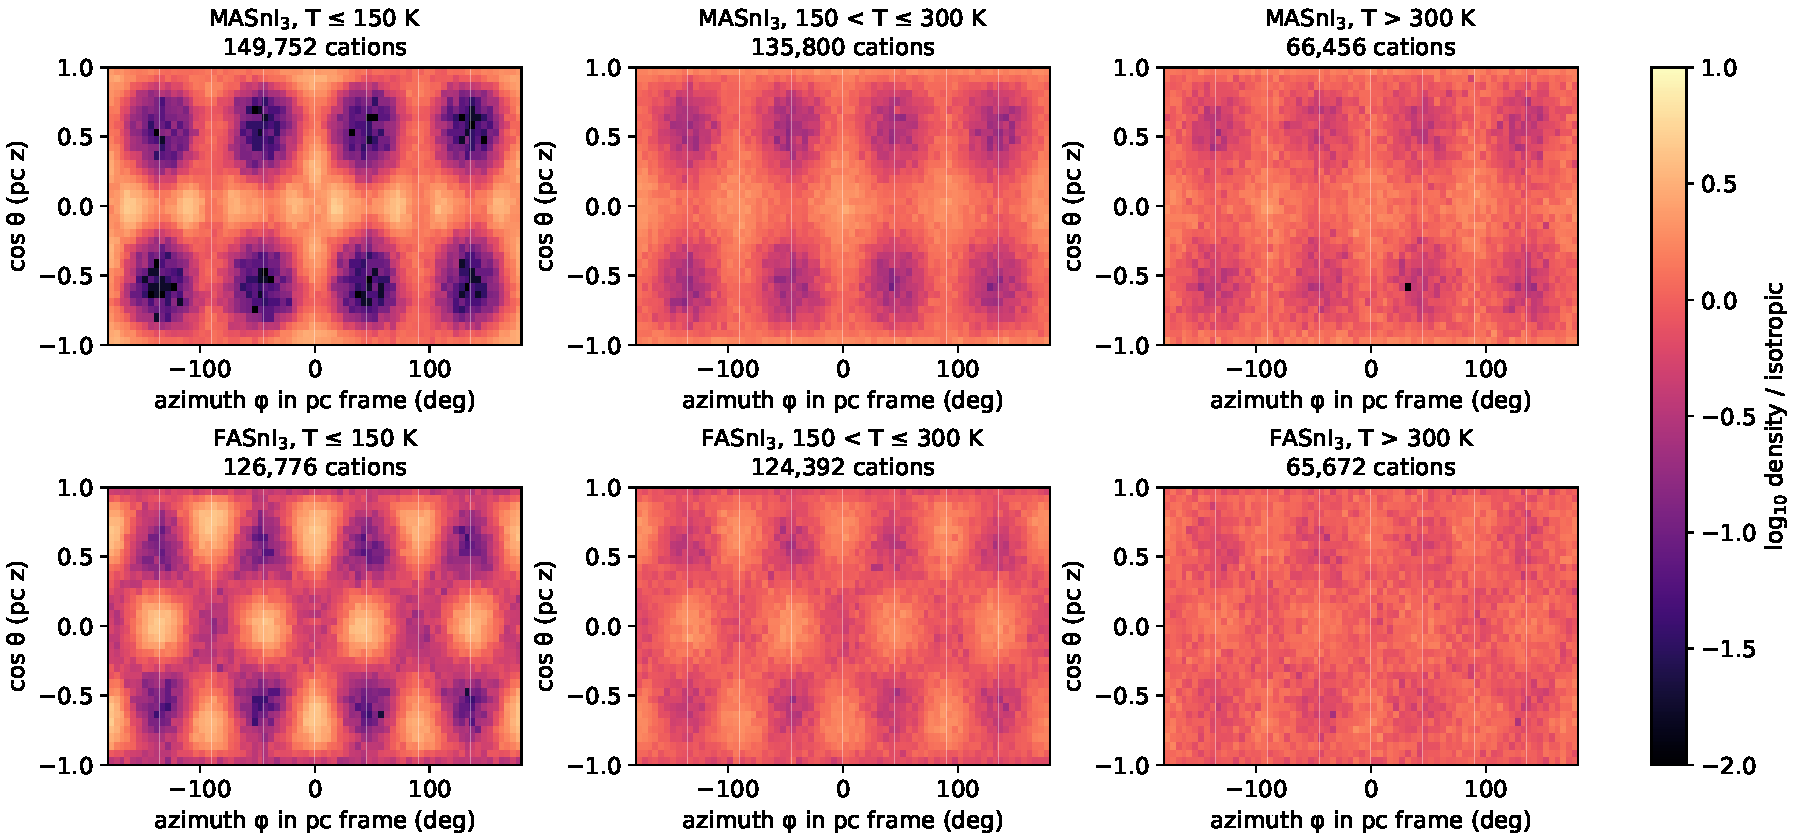
\includegraphics[width=\textwidth]{fig_dipole_sphere.pdf}
\caption{Orientation density of the molecular dipole axis (MA$^+$: C$\to$N; FA$^+$: N--N midpoint
$\to$C) in the pseudo-cubic frame, relative to an isotropic distribution (logarithmic colour scale),
for three temperature bands. Horizontal axis: azimuth; vertical axis: cosine of the polar angle, so
equal areas are equal solid angles.}
\label{fig:dipole_sphere}
\end{figure}

\begin{figure}[tb]
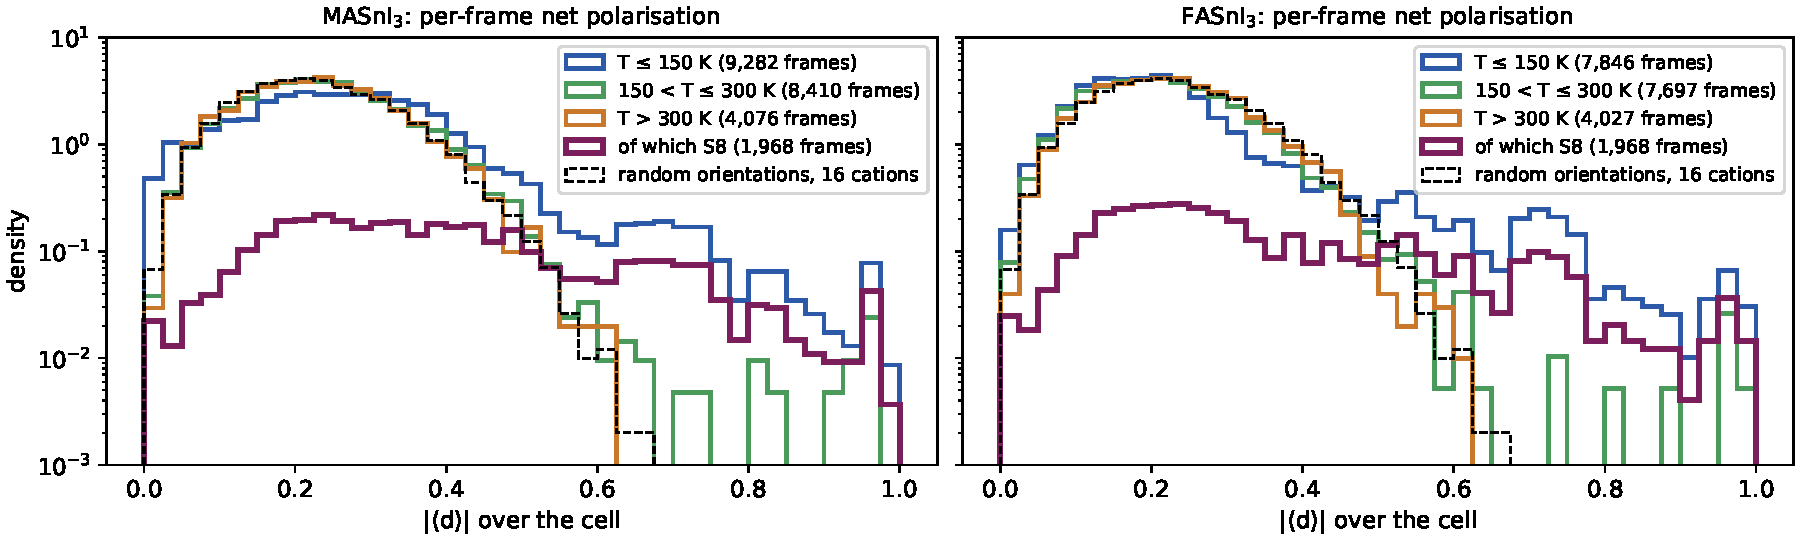
\includegraphics[width=\textwidth]{fig_dipole_polar.pdf}
\caption{Per-frame net polarisation $|\langle\mathbf{d}\rangle|$ of the molecular cations, for three
temperature bands (all stages), with the contribution of the dipole-targeted stage S8 (thick line)
and randomly oriented dipoles in a 16-cation cell (dashed). Logarithmic density scale.}
\label{fig:dipole_polar}
\end{figure}

\begin{figure}[tb]
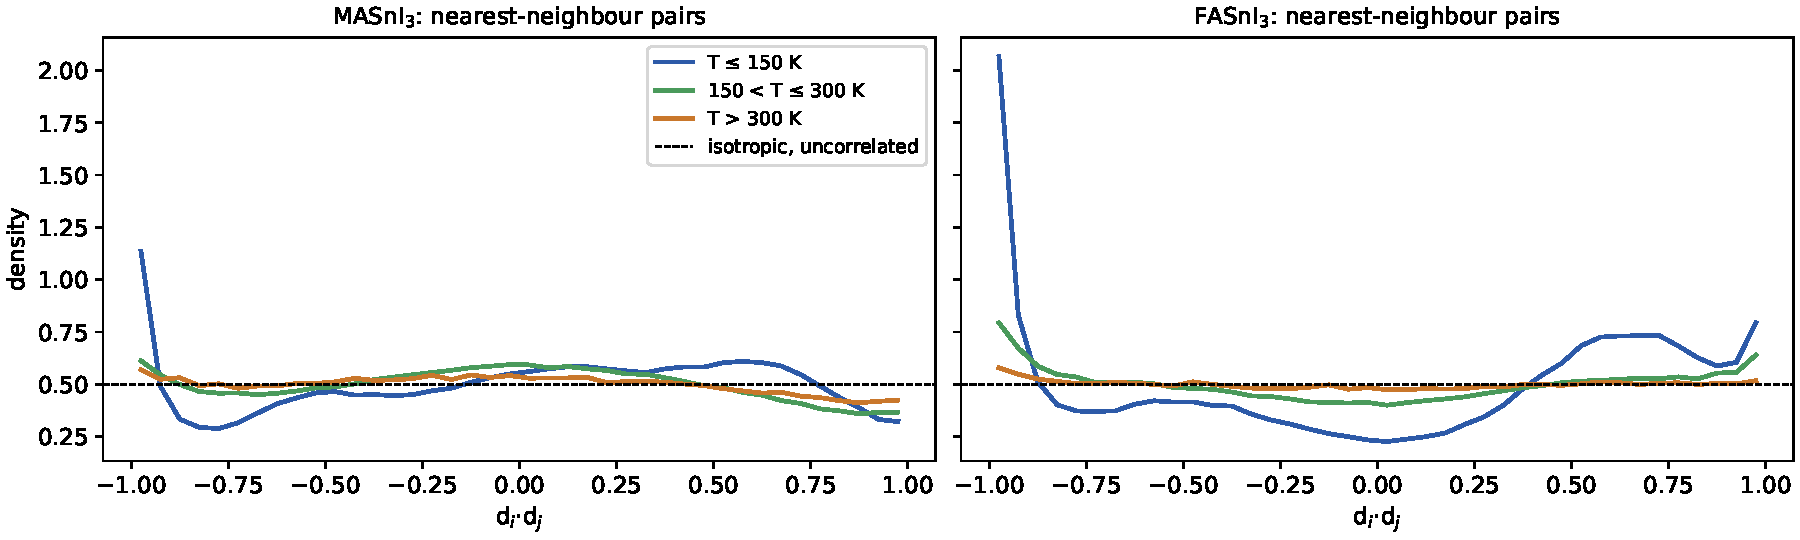
\includegraphics[width=\textwidth]{fig_dipole_pairs.pdf}
\caption{Distribution of the scalar product $\mathbf{d}_i\cdot\mathbf{d}_j$ of the dipole axes of
nearest-neighbour cation pairs in the pool, for \MASnI{} (left) and \FASnI{} (right) and three
temperature bands. The dashed line is the uniform density of isotropic, uncorrelated pairs. At and
below \SI{150}{\kelvin} antiparallel pairs ($\mathbf{d}_i\cdot\mathbf{d}_j\approx-1$) are enriched;
above it the distribution is close to uniform.}
\label{fig:dipole_pairs}
\end{figure}


%% ------------------------------------------------------------
\section{DFT settings and convergence}
\label{si:dftconv}
% Sources: PaperData/Task2_DFTcampaign/template.json, convergenceStudy/README.md (lines 100-125),
% plan-docs/Task1_configuration_generation_plan.md (PAW radii, line 285).
All labels are computed with the PAW datasets of the JTH table,\cite{Jollet2014CPC} using the
14-electron Sn dataset with the 4d states in the valence. The PAW radii are \SI{0.527}{\angstrom} (H),
\SI{0.798}{\angstrom} (C), \SI{0.638}{\angstrom} (N), \SI{1.329}{\angstrom} (Sn),
\SI{1.217}{\angstrom} (I) and \SI{1.168}{\angstrom} (Cs). The plane-wave cutoffs of
\SI{25}{\hartree} for the wave functions and \SI{250}{\hartree} for the density were chosen in a
convergence study on one cell of each compound (80 atoms of \CsSnI{}, 192 atoms of \MASnI{} and of
\FASnI{}) against a reference at \SI{60}{\hartree} and \SI{300}{\hartree} (Table~\ref{tab:si-conv}).
The targets were \SI{2e-4}{\hartree} per atom for the energy, \SI{2e-4}{\hartree\per\bohr} for the
root-mean-square force error and \SI{5e-6}{\hartree\per\bohr\cubed} for the largest stress component.
The total energy carries a nearly constant offset per Sn atom (\SI{2.2}{\milli\hartree} at
\SI{25}{\hartree}), which cancels in all energy differences, so the offset-corrected energy error is
the relevant one; with it, all three compounds meet every target. The convergence study was made with
PBEsol, and the same cutoffs are used for \rSCAN{}.

\begin{table}[htbp]
  \centering
  \caption{Errors of the label settings (\SI{25}{\hartree} / \SI{250}{\hartree}) against
    \SI{60}{\hartree} / \SI{300}{\hartree}.}
  \label{tab:si-conv}
  \begin{tabular}{lccccc}
    \toprule
    compound & $\Delta E$ total & $\Delta E$ offset-corrected & $\Delta F$ RMS & $\Delta F$ max & max $\Delta\sigma$ \\
             & (\si{\hartree}/atom) & (\si{\hartree}/atom) & (\si{\hartree\per\bohr}) & (\si{\hartree\per\bohr}) & (\si{\hartree\per\bohr\cubed}) \\
    \midrule
    \CsSnI{} & \num{5.7e-4} & \num{-2.7e-6} & \num{2.6e-6} & \num{1.2e-5} & \num{2.1e-6} \\
    \MASnI{} & \num{2.7e-4} & \num{2.3e-5} & \num{5.4e-5} & \num{2.0e-4} & \num{2.2e-6} \\
    \FASnI{} & \num{3.4e-4} & \num{3.7e-5} & \num{7.6e-5} & \num{3.6e-4} & \num{2.8e-6} \\
    \bottomrule
  \end{tabular}
\end{table}

% moved from the main text (2026-10-29, methods condensed)
The calculations use UrsaDFT (version 0.1.0) with plane waves. The Brillouin zone is sampled on $\Gamma$-centred
meshes with a spacing of \SI{0.2}{\per\angstrom} ($2\times2\times2$ for the 80-atom and $2\times2\times3$ for the
192-atom cells), and the occupations follow a Fermi--Dirac distribution at \SI{500}{K}. The self-consistent cycle is
converged to a density residual (L2 norm) of \num{e-5}; tightening it to \num{e-7} changes energies by
\SI{e-11}{\hartree} per atom, forces by \SI{2e-6}{\hartree\per\bohr} and stresses by less than
\SI{3e-9}{\hartree\per\bohr\cubed}. All calculations are in double precision. The initial PBEsol labels were computed
for 718 structures of 36 to 432 atoms, most of them cells of 160 or 192 atoms, and the initial \rSCAN{} labels for the
same structures and three further 360-atom cells of \CsSnI{}. These calculations ran on the AMD Instinct MI250X GPUs of
the Frontier supercomputer at the Oak Ridge Leadership Computing Facility (OLCF); the first 512 PBEsol structures took
on average 16.9 self-consistent iterations and about 114 node-hours in total.

\paragraph{Spin--orbit coupling.}
No calculation in this work includes spin--orbit coupling (SOC). In tin halide
perovskites SOC lowers the conduction-band minimum and reduces the gap by
several tenths of an eV,\cite{ref_soc_sn} so absolute gaps without SOC are not
meaningful and none is reported as a result. We report only gap differences
between matched states of the same compound, \dEg{}. This rests on the
assumption that the SOC correction to the gap is the same in the two states
being compared. The states compared here differ by strains below
\SI{1}{\percent}, by tilt angles of a few degrees and by cation orientations,
and we expect the SOC shift to change much less than the gap itself across
such states; this assumption is not tested here.

%% ------------------------------------------------------------
\section{Force-field training and validation}
\label{si:ff}
% Sources: model file header (Task4_PhaseTransition/model/nep_modelA.txt), Task3_MLFF_scratch/ft_gen87large/finetune.yaml,
% mace/mh1/train.log, mace/omat_medium/train.log; generated tables: PaperData/paper_figs/si_ff_tables.py.
% moved from the main text (2026-10-29, methods condensed)
\paragraph{Labels and data split.}
The energy labels are cohesive energies: the DFT free energy minus the free energies of the
isolated atoms computed with the same settings. Forces and the full stress tensor are fitted as
well. The labelled structures are split by MD trajectory, so that all frames of one trajectory
fall into the same subset, and stratified by compound, with a fixed seed: 555 structures from 228
trajectories for training, 60 from 30 trajectories for validation and 100 from 44 trajectories
held out. By compound, \CsSnI{}, \MASnI{}, \FASnI{} and the reference compounds contribute 105,
247, 190 and 13 training structures, 12, 27, 21 and 0 validation structures, and 19, 46, 35 and 0
held-out structures. The \rSCAN{} potentials use the same split without the excluded structures
(546, 60 and 99). All six potentials are trained on the training set, the validation set monitors
the training, and the held-out set is used for the assessment below.

\paragraph{MACE.}
Both MACE models have two message-passing layers with correlation order 3 and angular resolution
$l = 3$, a radial cutoff of \SI{6}{\angstrom} (receptive field \SI{12}{\angstrom}), and 512
(MACE-MH-1) or 128 (MACE-OMAT) channels per irreducible representation. MACE-MH-1 is a
multi-head model; its fine-tuning starts from the head trained on PBE data of the OMat set for the
PBEsol labels and from the head trained on \rSCAN{} data of the MatPES set for the \rSCAN{}
labels. Both models were fine-tuned for 200 epochs in double precision with the AMSGrad variant of
Adam, a learning rate of \num{e-3}, batches of four structures, an exponential moving average of
the weights (decay 0.99) and loss weights of 1, 100 and 10 for energies, forces and stresses. The
reference atomic energies are set to zero because the labels are cohesive energies.

\paragraph{UrsaMLFF.}
UrsaMLFF describes each atom by radial and angular descriptors with cutoffs of \SI{8}{\angstrom}
and \SI{6}{\angstrom}, built from Chebyshev radial basis sets of size 16 and 12 with 8 and 6 radial
functions, and angular terms up to $l = 4$ for three-body and $l = 2$ and 1 for four- and
five-body correlations; a Ziegler--Biersack--Littmark repulsion is added at short range. One hidden
layer of 120 neurons per element maps the descriptors to atomic energies. The weights were
initialised from our in-house general-purpose model of the same architecture, trained on 87
elements of a public 89-element data set\cite{Song2024NEP89} and reduced to H, C, N, Sn, I and Cs,
and fine-tuned with Adam in batches of 64 structures for \num{10000} epochs. For the first 1500
epochs the learning rate is \num{5e-3} and the loss weights of energy, forces and virial are 1,
100 and 1; thereafter the learning rate is \num{5e-4} and the weights are 100, 50 and 30. The
PBEsol potential was chosen among five candidates (this one, a fine-tuned public foundation model
and three potentials trained from random initialisation) by the force error on the held-out set,
which makes its held-out errors slightly optimistic; its validation errors
(\SI{1.11e-4}{\hartree} per atom, \SI{1.03e-3}{\hartree\per\bohr} and
\SI{1.79e-6}{\hartree\per\bohr\cubed}) are of the same size. The \rSCAN{} potential was trained with
the identical protocol. Training takes about \SI{1.2}{h} on one A100 GPU.

\paragraph{Accuracy on held-out structures.}
Tables~\ref{tab:holdout} (main text, \rSCAN{}) and~\ref{tab:si-holdout-pbesol} (PBEsol) and Figures~\ref{fig:parity} and~\ref{fig:si-parity-pbesol} compare the six potentials on the held-out
structures\changed{; for UrsaMLFF these are the potentials retrained as described below}. All reproduce the
DFT forces with $R^2 \ge 0.99$ and the energies within a compound with \changed{$R^2 \ge 0.98$}. The MACE
models reproduce the forces \changed{2.4 to 2.7 times more accurately than UrsaMLFF with PBEsol labels and 1.9
to 2.1 times more accurately with \rSCAN{} labels}, while UrsaMLFF reproduces the stresses \changed{better, by
factors of 2.6 to 2.7 with PBEsol and 2.3 to 4.7 with \rSCAN{} labels}; the stress error of the MACE models is
dominated by a constant pressure offset. Every model fits the \rSCAN{} labels slightly less accurately than
the PBEsol labels, except for the stress\changed{es} of MACE-OMAT\changed{ and UrsaMLFF; the PBEsol UrsaMLFF is
in addition trained on the refined data, which have no \rSCAN{} counterpart (below)}.

% generated by PaperData/paper_figs/fig_holdout.py; do not edit
\begin{table}[htbp]
\centering
\caption{Errors of the potentials trained on the PBEsol labels on the 100 held-out structures: root-mean-square errors of the energy per atom, the force components and the stress components, and coefficients of determination $R^2$ (for the energy after subtracting the mean DFT energy of each compound). UrsaMLFF: potential retrained on the refined training data; MACE: fine-tuned on the 555 initial structures.}
\label{tab:si-holdout-pbesol}
\resizebox{\linewidth}{!}{%
\begin{tabular}{lcccccc}
\toprule
model & $E$ (\si{\hartree}/atom) & $F$ (\si{\hartree\per\bohr}) & $\sigma$ (\si{\hartree\per\bohr\cubed}) & $R^2_E$ & $R^2_F$ & $R^2_\sigma$ \\
\midrule
\changed{UrsaMLFF} & \changed{\num{6.23e-5}} & \changed{\num{5.15e-4}} & \changed{\num{9.11e-7}} & \changed{0.9940} & \changed{0.9986} & \changed{0.9959} \\
MACE-MH-1 & \num{3.29e-5} & \num{1.94e-4} & \num{2.46e-6} & 0.9983 & 0.9998 & 0.9705 \\
MACE-OMAT & \num{7.99e-5} & \num{2.15e-4} & \num{2.37e-6} & 0.9901 & 0.9998 & 0.9727 \\
\bottomrule
\end{tabular}}
\end{table}


\begin{figure}[htbp]
  \centering
  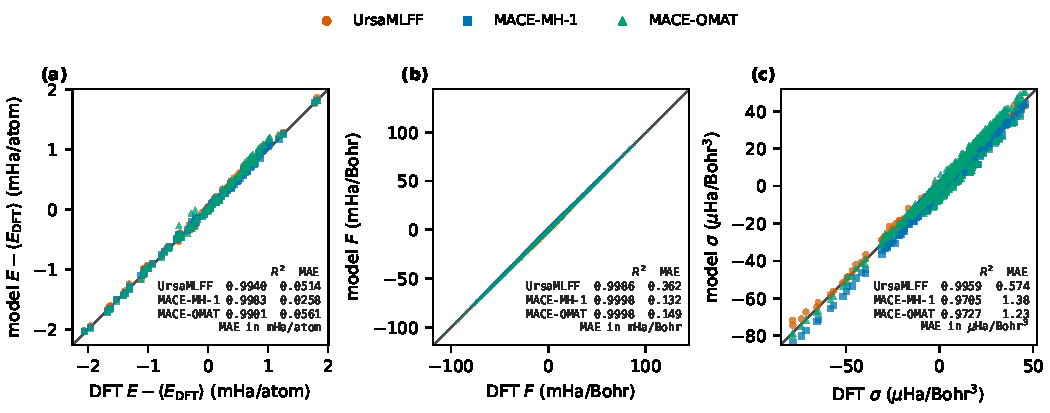
\includegraphics[width=\linewidth]{figures/fig_parity_pbesol.pdf}
  \caption{\changed{Predicted against DFT values on the 100 held-out structures for the potentials trained on the PBEsol
    labels; panels and insets as in Figure~\ref{fig:parity}. UrsaMLFF is the potential retrained on the refined training
    data.}}
  \label{fig:si-parity-pbesol}
\end{figure}

{\changedcolor
% Sources: Task3_MLFF_scratch/al_round3 (full_pbesol_dataset_al3.extxyz: 212 new labels; v2_balanced/, balanced_al3_s1),
% Task4_PhaseTransition/npt_v2_check (score_engine.md: errors; md integrity of every campaign), FinalData/README.md.
% (User 2026-10-27: present one force field; the refinement is described here only.)
\paragraph{Refinement of the training data.}
MD of the hybrids with the production protocol revealed molecular dissociation: protons detached from
their cation, broken C--N bonds and two cations in one cage, in configurations whose energies UrsaMLFF
placed 1 to \SI{2e-3}{\hartree} per atom below DFT (Table~\ref{tab:si-ood}). We therefore added DFT
labels of such configurations in three rounds of active learning. Each round cut 192-atom cells around
the defect events of the hybrid MD, re-equilibrated their surroundings with the defect core fixed, and
added images in which one N--H or C--H bond is stretched to between 1.03 and \SI{1.6}{\angstrom}.
Together with 27 frames of earlier out-of-distribution MD, 212 new structures were labelled with the
settings above; 210 join the training set and two the held-out set, which then hold 765 and 102
structures (60 for validation). UrsaMLFF was retrained on the refined data, with one equivariant
message-passing step added to its descriptors (radial and angular cutoffs of 6 and \SI{5}{\angstrom},
one hidden layer of 64 neurons, 49\,391 parameters), from random initialisation for 1000 epochs, and
the retrained candidate kept is the one whose MD of the hybrids remained free of molecular defects.
Its errors on the training, validation and held-out sets are \SI{4.7e-5}{}, \SI{6.4e-5}{} and
\SI{6.2e-5}{\hartree} per atom for energies and \SI{5.0e-4}{}, \SI{4.6e-4}{} and
\SI{5.3e-4}{\hartree\per\bohr} for forces, with stress errors of \SI{7.7e-7}{} and
\SI{1.2e-6}{\hartree\per\bohr\cubed} on the validation and held-out sets; on the 100 held-out structures
shared with the other potentials (Table~\ref{tab:holdout}, Figure~\ref{fig:parity}) they are
\SI{6.2e-5}{\hartree} per atom, \SI{5.2e-4}{\hartree\per\bohr} and \SI{9.1e-7}{\hartree\per\bohr\cubed}.
\changed{The final \rSCAN{} potential was trained in the same way, for 3000 epochs, on the \rSCAN{} training set of
866 structures, which holds the 546 initial structures, 203 active-learning structures and the 117 further
structures described in section~\ref{sec:configgen:al}; of three seeds, the one with the lower validation force error
was kept. Its errors on the validation set and on the 99 held-out structures shared with the MACE models are
\SI{8.5e-5}{} and \SI{9.2e-5}{\hartree} per atom for energies, \SI{4.6e-4}{} and \SI{5.2e-4}{\hartree\per\bohr} for
forces and \SI{8.0e-7}{} and \SI{8.5e-7}{\hartree\per\bohr\cubed} for stresses.} The transition temperatures of \MASnI{} and \FASnI{},
the clamping study of the hybrids and the comparison of exchange--correlation functionals use the
retrained potentials; the production runs of \CsSnI{} and the cell-size study with \rSCAN{} labels in the
Supporting Information use the potentials trained before the refinement.
}

Table~\ref{tab:si-hyper} lists the architectures and training settings of the two classes of
potentials described in the main text. Table~\ref{tab:si-holdout-material} breaks the held-out errors
down by compound. For UrsaMLFF \changed{(the retrained potentials) the energy and stress errors are largest
for \FASnI{}}; the MACE models have their largest
stress errors mostly for \CsSnI{}, in line with the constant pressure offset noted in the main text.
The force errors of each potential vary by less than half between the compounds.

The production UrsaMLFF was chosen among five candidates of the same architecture that differ in
their initial weights (Table~\ref{tab:si-candidates}): fine-tuning from our in-house general-purpose
model, fine-tuning from a public foundation model, and training from random initialisation with three
seeds. The candidate fine-tuned from the in-house model has the lowest force error on the held-out
set and was selected on that basis, which makes its held-out errors slightly optimistic. The
candidates trained from random initialisation have force errors of 1.30 to
\SI{1.33e-3}{\hartree\per\bohr}, against \SI{1.17e-3}{\hartree\per\bohr} for the selected
potential, and energy and stress errors of similar size. Both MACE models reproduce the forces at
least five times more accurately than any UrsaMLFF candidate.

Table~\ref{tab:si-ood} gives the test of whether MD with each potential stays within the training
data. On frames from MACE runs, and on all \CsSnI{} frames, the force disagreement between UrsaMLFF and
MACE-MH-1 is close to its value on the held-out set. On frames from the UrsaMLFF runs of the hybrids it
is 1.5 to 1.6 times larger for \MASnI{} and 2.9 to 3.3 times larger for \FASnI{}, and the energy of
UrsaMLFF lies 0.5 to \SI{1.6e-3}{\hartree} per atom below that of MACE-MH-1. The DFT calculations on
such frames reported in the main text confirm that these configurations lie outside the training data
of UrsaMLFF.

\begin{table}[htbp]
  \centering\small
  \caption{Architectures and training settings of the fine-tuned potentials. The same settings are
    used for the PBEsol and the \rSCAN{} labels.}
  \label{tab:si-hyper}
  \begin{tabular}{lp{0.36\linewidth}p{0.36\linewidth}}
    \toprule
    & UrsaMLFF & MACE-MH-1 / MACE-OMAT \\
    \midrule
    descriptors & radial and angular, cutoffs \SI{8}{\angstrom} and \SI{6}{\angstrom}; Chebyshev basis of
      size 16 and 12 with 8 and 6 radial functions; angular order 4 (three-body), 2 (four-body) and 1
      (five-body) & two equivariant message-passing layers, correlation order 3, $l = 3$; radial cutoff
      \SI{6}{\angstrom}, receptive field \SI{12}{\angstrom} \\
    network & one hidden layer of 120 neurons per element; Ziegler--Biersack--Littmark repulsion at short
      range & 512 (MH-1) or 128 (OMAT) channels per irreducible representation \\
    initial weights & in-house general-purpose model (87 elements), reduced to H, C, N, Sn, I, Cs &
      MACE-MH-1 (head of OMat PBE data for PBEsol, of MatPES \rSCAN{} data for \rSCAN{}) or
      MACE-OMAT-0-medium \\
    optimiser & Adam, batches of 64 structures, \num{10000} epochs & AMSGrad, batches of 4 structures,
      200 epochs, weight average with decay 0.99 \\
    learning rate & \num{5e-3} for epochs 0--1500, then \num{5e-4} & \num{e-3} \\
    loss weights $E$/$F$/$\sigma$ & 1/100/1, then 100/50/30 & 1/100/10 \\
    precision & double & double (training), single (MD) \\
    \bottomrule
  \end{tabular}
\end{table}

% generated by PaperData/paper_figs/si_ff_tables.py; do not edit
\begin{table}[htbp]
\centering\small
\caption{Root-mean-square errors on the held-out structures, by compound, for the six fine-tuned potentials. \changed{UrsaMLFF is the retrained potential of Table~\ref{tab:holdout}.}}
\label{tab:si-holdout-material}
\resizebox{\linewidth}{!}{%
\begin{tabular}{lllccc}
\toprule
labels & model & compound (structures) & $E$ (\si{\hartree}/atom) & $F$ (\si{\hartree\per\bohr}) & $\sigma$ (\si{\hartree\per\bohr\cubed}) \\
\midrule
PBEsol & UrsaMLFF & \CsSnI{} (19) & \changed{\num{4.35e-5}} & \changed{\num{5.36e-4}} & \changed{\num{6.69e-7}} \\
 &  & \MASnI{} (46) & \changed{\num{4.41e-5}} & \changed{\num{5.03e-4}} & \changed{\num{7.36e-7}} \\
 &  & \FASnI{} (35) & \changed{\num{8.66e-5}} & \changed{\num{5.21e-4}} & \changed{\num{1.19e-6}} \\
 & MACE-MH-1 & \CsSnI{} (19) & \num{3.07e-5} & \num{2.60e-4} & \num{3.58e-6} \\
 &  & \MASnI{} (46) & \num{1.83e-5} & \num{1.79e-4} & \num{2.33e-6} \\
 &  & \FASnI{} (35) & \num{4.62e-5} & \num{1.79e-4} & \num{1.78e-6} \\
 & MACE-OMAT & \CsSnI{} (19) & \num{8.65e-5} & \num{2.66e-4} & \num{4.00e-6} \\
 &  & \MASnI{} (46) & \num{4.15e-5} & \num{2.02e-4} & \num{1.31e-6} \\
 &  & \FASnI{} (35) & \num{1.09e-4} & \num{2.08e-4} & \num{2.25e-6} \\
\midrule
\rSCAN{} & UrsaMLFF & \CsSnI{} (18) & \changed{\num{6.25e-5}} & \changed{\num{6.13e-4}} & \changed{\num{6.83e-7}} \\
 &  & \MASnI{} (46) & \changed{\num{8.20e-5}} & \changed{\num{5.09e-4}} & \changed{\num{6.94e-7}} \\
 &  & \FASnI{} (35) & \changed{\num{1.21e-4}} & \changed{\num{5.15e-4}} & \changed{\num{7.44e-7}} \\
 & MACE-MH-1 & \CsSnI{} (18) & \num{3.86e-5} & \num{3.00e-4} & \num{3.99e-6} \\
 &  & \MASnI{} (46) & \num{1.68e-5} & \num{2.23e-4} & \num{3.92e-6} \\
 &  & \FASnI{} (35) & \num{6.52e-5} & \num{2.55e-4} & \num{4.14e-6} \\
 & MACE-OMAT & \CsSnI{} (18) & \num{5.71e-5} & \num{3.06e-4} & \num{4.14e-6} \\
 &  & \MASnI{} (46) & \num{5.92e-5} & \num{2.44e-4} & \num{1.07e-6} \\
 &  & \FASnI{} (35) & \num{1.44e-4} & \num{2.79e-4} & \num{9.44e-7} \\
\bottomrule
\end{tabular}}
\end{table}

% generated by PaperData/paper_figs/si_ff_tables.py; do not edit
\begin{table}[htbp]
\centering\small
\caption{Held-out errors (100 structures, PBEsol labels) of the five UrsaMLFF candidates, which share the architecture and differ in their initial weights, and of the two MACE models. $F_\mathrm{max}$: largest force-component error.}
\label{tab:si-candidates}
\resizebox{\linewidth}{!}{%
\begin{tabular}{lcccc}
\toprule
potential & $E$ (\si{\hartree}/atom) & $F$ (\si{\hartree\per\bohr}) & $\sigma$ (\si{\hartree\per\bohr\cubed}) & $F_\mathrm{max}$ (\si{\hartree\per\bohr}) \\
\midrule
UrsaMLFF, fine-tuned from the in-house general-purpose model (production) & \num{7.99e-5} & \num{1.17e-3} & \num{1.74e-6} & \num{2.86e-2} \\
fine-tuned from the public foundation model (stopped after 5984 epochs) & \num{9.04e-5} & \num{1.32e-3} & \num{2.35e-6} & \num{2.09e-2} \\
random initialisation, seed 1 & \num{8.75e-5} & \num{1.33e-3} & \num{1.93e-6} & \num{3.64e-2} \\
random initialisation, seed 2 & \num{6.77e-5} & \num{1.32e-3} & \num{1.79e-6} & \num{1.94e-2} \\
random initialisation, seed 3 & \num{5.91e-5} & \num{1.30e-3} & \num{1.49e-6} & \num{2.43e-2} \\
MACE-MH-1, fine-tuned & \num{3.29e-5} & \num{1.94e-4} & \num{2.46e-6} & \num{2.43e-3} \\
MACE-OMAT, fine-tuned & \num{7.99e-5} & \num{2.15e-4} & \num{2.37e-6} & \num{2.22e-3} \\
\bottomrule
\end{tabular}}
\end{table}

% generated by PaperData/paper_figs/si_ff_tables.py; do not edit
\begin{table}[htbp]
\centering\small
\caption{Force disagreement between UrsaMLFF and MACE-MH-1 (PBEsol labels, without D3) on frames of the 960- and 864-atom D3 ramps, relative to their disagreement on the held-out set of the same compound. Absolute: ratio of the root-mean-square force differences; relative: the same for the difference divided by the force magnitude, which removes the temperature scaling. $\Delta E$: energy of UrsaMLFF minus that of MACE-MH-1 per atom, relative to its held-out mean.}
\label{tab:si-ood}
\resizebox{\linewidth}{!}{%
\begin{tabular}{lllcccc}
\toprule
compound & frames from & $T$ (K) & frames & absolute & relative & $\Delta E$ (\si{\hartree}/atom) \\
\midrule
\MASnI{} & UrsaMLFF runs & 50--150 & 147 & 1.48 & 3.18 & \num{-6.30e-4} \\
 & UrsaMLFF runs & 150--250 & 150 & 1.57 & 2.31 & \num{-5.90e-4} \\
 & UrsaMLFF runs & 250--400 & 225 & 1.59 & 1.75 & \num{-4.80e-4} \\
 & MACE runs & 50--150 & 98 & 0.52 & 1.14 & \num{-1.90e-5} \\
 & MACE runs & 150--250 & 100 & 0.65 & 0.99 & \num{8.00e-6} \\
 & MACE runs & 250--400 & 150 & 0.80 & 0.91 & \num{2.10e-5} \\
\FASnI{} & UrsaMLFF runs & 50--150 & 147 & 2.94 & 5.18 & \num{-1.50e-3} \\
 & UrsaMLFF runs & 150--250 & 150 & 3.13 & 3.85 & \num{-1.60e-3} \\
 & UrsaMLFF runs & 250--400 & 225 & 3.30 & 3.15 & \num{-1.60e-3} \\
 & MACE runs & 50--150 & 98 & 0.66 & 1.33 & \num{-2.70e-6} \\
 & MACE runs & 150--250 & 100 & 0.78 & 1.07 & \num{-1.90e-6} \\
 & MACE runs & 250--400 & 150 & 0.92 & 0.95 & \num{-1.10e-6} \\
\CsSnI{} & UrsaMLFF runs & 200--350 & 224 & 0.76 & 0.90 & \num{-1.20e-4} \\
 & UrsaMLFF runs & 350--450 & 150 & 0.89 & 0.88 & \num{-1.00e-4} \\
 & UrsaMLFF runs & 450--600 & 222 & 0.99 & 0.86 & \num{-8.80e-5} \\
 & MACE runs & 200--350 & 150 & 0.73 & 0.90 & \num{-3.40e-5} \\
 & MACE runs & 350--450 & 100 & 0.86 & 0.88 & \num{-4.60e-6} \\
 & MACE runs & 450--600 & 148 & 0.97 & 0.87 & \num{2.20e-5} \\
\bottomrule
\end{tabular}}
\end{table}


% moved from the main text (2026-10-29, methods condensed)
\paragraph{Throughput.}
% Source: PaperData/paper_figs/fig_throughput.py (benchmark Task4_PhaseTransition/bench_throughput).
Accuracy is only one requirement; the production MD of this work, about \SI{45}{ns} in cells of
2000 to 4900 atoms plus the cell-size tests, also needs speed. Figure~\ref{fig:throughput} shows
the MD throughput of the three potentials on one A100 GPU, with D3, for cells below 500 atoms,
between 500 and 1000 atoms, of about 2000 atoms and of about $10^4$ atoms, each measured alone on an
otherwise idle GPU; Table~\ref{tab:si-throughput} lists the values. Up to 2300 atoms, UrsaMLFF runs 960 to 2540 MD steps per second and the MACE
models 7 to 25; at $10^4$ atoms, UrsaMLFF runs 550 to 1140 steps per second and the MACE models 1.7
to 4.7. UrsaMLFF is thus 70 to 135 times faster than the faster MACE model up to 2300 atoms and about
240 times faster at $10^4$ atoms. In the production cells this means 386 (\CsSnI{}) and
\SI{83}{ns} (\MASnI{}) per day for UrsaMLFF against 2.9 and \SI{0.84}{ns} per day for MACE-OMAT.
At the measured rates, the production MD of this work takes about \SI{10}{h} of GPU time with
UrsaMLFF, against about 40 days with MACE-OMAT and 59 days with MACE-MH-1. This is why UrsaMLFF
carries the production simulations although its force error is \changed{two to three times larger}; the MACE
models serve to validate it \changed{(Table~\ref{tab:holdout} and section \emph{Transition temperatures
compared with experiment})}.

\begin{figure}[htbp]
  \centering
  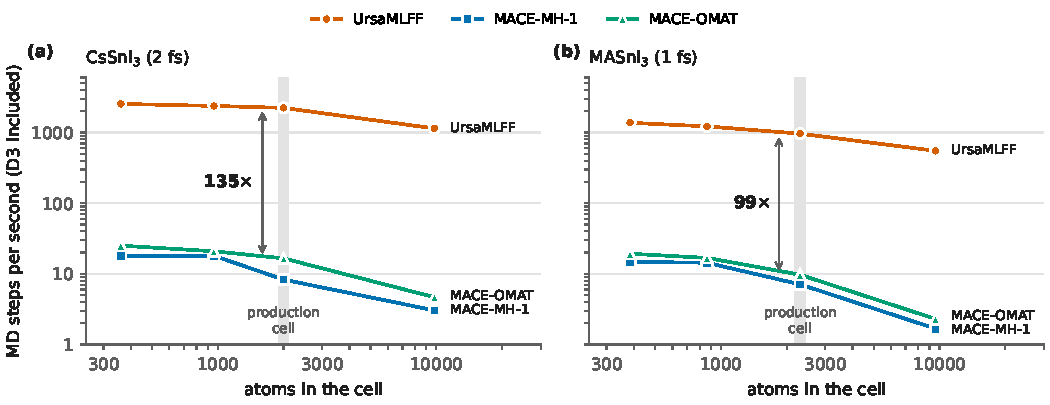
\includegraphics[width=\linewidth]{fig_throughput}
  \caption{MD throughput of the fine-tuned potentials on one NVIDIA A100 GPU, including D3, against
    the number of atoms in the cell: (a) \CsSnI{}, (b) \MASnI{}. UrsaMLFF runs in the production MD
    engine in double precision, the MACE models in the MD driver of the model comparison in single
    precision. Each value was measured alone on an otherwise idle GPU. Grey band: production cell;
    arrow: speed-up of UrsaMLFF over the faster MACE model in that cell. The values, with the
    corresponding nanoseconds per day, are listed in Table~\ref{tab:si-throughput}.}
  \label{fig:throughput}
\end{figure}

Table~\ref{tab:si-throughput} lists the MD throughput values shown in Figure~\ref{fig:throughput},
with the corresponding simulated time per day at the production time steps.

% generated by PaperData/paper_figs/fig_throughput.py; do not edit
\begin{table}[htbp]
\centering
\caption{MD throughput of the fine-tuned potentials on one NVIDIA A100 GPU, in MD steps per second, including D3. UrsaMLFF: the production MD engine, one system per GPU, double precision. MACE: the MD driver used for the model comparison, single precision. In brackets: nanoseconds per day at the production time steps (\SI{2}{fs} for \CsSnI{}, \SI{1}{fs} for the hybrids). Each value was measured alone on an otherwise idle GPU.}
\label{tab:si-throughput}
\resizebox{\linewidth}{!}{%
\begin{tabular}{llcccc}
\toprule
\multicolumn{6}{l}{\CsSnI{}} \\
model & & 360 atoms & 960 atoms & 2000 atoms & 9800 atoms \\ \midrule
UrsaMLFF &  & 2541 (4.4e+02) & 2379 (4.1e+02) & 2232 (3.9e+02) & 1141 (2e+02) \\
MACE-MH-1 &  & 18 (3.1) & 18 (3.1) & 8.3 (1.4) & 3 (0.53) \\
MACE-OMAT &  & 25 (4.3) & 21 (3.6) & 17 (2.9) & 4.7 (0.81) \\
\midrule
\multicolumn{6}{l}{\MASnI{}} \\
model & & 384 atoms & 864 atoms & 2304 atoms & 9600 atoms \\ \midrule
UrsaMLFF &  & 1374 (1.2e+02) & 1221 (1.1e+02) & 964 (83) & 550 (48) \\
MACE-MH-1 &  & 15 (1.3) & 14 (1.2) & 7.1 (0.61) & 1.7 (0.15) \\
MACE-OMAT &  & 19 (1.7) & 17 (1.5) & 9.7 (0.84) & 2.3 (0.2) \\
\bottomrule
\end{tabular}}
\end{table}


%% ------------------------------------------------------------
\section{Phase-transition protocol}
\label{si:models}
% Sources: PaperData/Task4_PhaseTransition/README.md (model comparison, driver check, D3), make_campaign.py,
% make_size.py, DFTengine/r2scan_bugfix_work/pulay/pulay.md.
All heating and cooling ramps of this work, that is, the comparison of the six fine-tuned potentials,
the cell-size study and the production cells, follow one protocol, and only the cell size changes. The
cells are supercells of the $\sqrt2\times\sqrt2\times2$ setting: 960 atoms for \CsSnI{}
($4\times4\times3$) and 864 atoms for \MASnI{} and \FASnI{} ($3\times3\times2$) in the model
comparison, and 360 to 4900 atoms for \CsSnI{} and 384 to 4800 atoms for the hybrids in the cell-size
study, which includes the production cells of 2000 ($5\times5\times4$) and 2304 atoms
($4\times4\times3$). The time step is \SI{2}{fs} for \CsSnI{} and \SI{1}{fs} for the hybrids. Each
run starts with a FIRE minimisation at fixed cell, followed by \SI{5}{ps} at constant volume and
\SI{20}{ps} at constant pressure at the start temperature, and continues with a linear temperature
ramp at \SI{2}{K/ps} between \SI{200}{K} and \SI{600}{K} for \CsSnI{} or between \SI{50}{K} and
\SI{400}{K} for the hybrids. Heating runs start from the orthorhombic structure and cooling runs from
the cubic structure. \changed{For the hybrids with the retrained UrsaMLFF, the cell of the orthorhombic
starting structure is first set, by an affine scaling, to the mean cell of the model at \SI{50}{K} in the
same cell size (main text, \emph{Starting structure of the hybrid heating runs}). The 18\,432-atom runs
($8\times8\times6$) follow the same protocol at \SI{1}{K/ps}. The holds that bracket the equilibrium tilt loss
of \MASnI{} (2304 atoms) last \SI{150}{ps} at 250, 265 and \SI{280}{K}; they start either from the crystal
prepared in the \SI{50}{K} cell and heated to the hold temperature at \SI{5}{K/ps}, or from the heating frame
of a production run closest to the hold temperature, in the cubic phase.} Temperature is controlled by stochastic velocity rescaling with a time constant
of \SI{100}{fs}, and pressure by stochastic cell rescaling with independent axes and a time constant
of \SI{1}{ps}.

Dispersion is included with D3 and Becke--Johnson damping, using the parameters of the training
functional (PBEsol: $s_6 = 1$, $s_8 = 2.9491$, $a_1 = 0.4466$, $a_2 = \SI{6.1742}{\angstrom}$;
\rSCAN{}: $s_6 = 1$, $s_8 = 0.78981$, $a_1 = 0.49484$, $a_2 = \SI{5.73084}{\angstrom}$), a pair cutoff
of \SI{15}{\angstrom} and a coordination-number cutoff of \SI{6}{\angstrom}. UrsaMLFF is run five times
per compound, direction and cell size at the external pressure $P_\mathrm{ext}$ of its functional:
$-0.065$, $-0.043$ and \SI{-0.058}{GPa} for \CsSnI{}, \MASnI{} and \FASnI{} with PBEsol and $-0.039$,
$-0.150$ and \SI{-0.183}{GPa} with \rSCAN{}. Each MACE model is run once, at zero
pressure. The transition temperatures are determined with the criterion of the main text
(\emph{Phase identification and transition temperatures}).

The MACE runs use an MD driver built on ASE\cite{Larsen2017ASE} that implements the thermostat and
barostat of the engine, with the MACE models evaluated in single precision and D3 evaluated on the
GPU. We validated the driver against the engine with the PBEsol UrsaMLFF in three runs of
\SI{100}{ps} at \SI{400}{K}: the temperature and volume fluctuations and the cell shape agree, and the
mean volume is \SI{0.16}{\percent} lower, equivalent to a pressure difference of less than
\SI{20}{MPa}. The D3 implementation of the driver agrees with that of the engine to better than
\SI{4e-9}{\hartree} per atom.

% moved from the main text (2026-10-29, methods condensed)
\paragraph{Engine and cells.} MD is run with the GPU engine of UrsaMLFF, which evaluates the force field and D3 in
double precision (version 0.1.0, development build of commit 52159a3). The barostat compressibility is set from a bulk
modulus of \SI{15}{GPa}, and structures are minimised with FIRE\cite{Bitzek2006PRL} before the first MD stage. Because
the cubic, tetragonal and orthorhombic phases are all orthogonal in the $\sqrt{2}\times\sqrt{2}\times2$ setting, every
transition can proceed by rescaling the three axes, at the price that the tetragonal axis is favoured along the cell's
$c$ axis. Pseudo-cubic lattice constants are $a/(\sqrt{2}n_1)$, $b/(\sqrt{2}n_2)$ and $c/(2n_3)$ for an
$n_1\times n_2\times n_3$ supercell.

\paragraph{Heating and cooling ramps.}
Each ramp starts with a FIRE minimisation at fixed cell, \SI{5}{ps} of
constant-volume MD and \SI{20}{ps} of constant-pressure MD at the start
temperature, followed by a linear temperature ramp at \SI{2}{K/ps} at constant
pressure. \CsSnI{} is heated from the $\gamma$ ($Pnma$) structure from
\SI{200}{K} to \SI{600}{K} and cooled from the cubic structure from
\SI{600}{K} to \SI{200}{K}. \MASnI{} and \FASnI{} are heated from orthorhombic
structures and cooled from cubic structures with randomly oriented cations
between \SI{50}{K} and \SI{400}{K}. The heating runs start from the Materials Project
$Pnma$ structure of \CsSnI{} (mp-568570) at the experimental lattice,\cite{Chung2012JACS} the
$Pnma$ structure of \MASnI{} with antipolar MA order (mp-1094059), and an $a^-a^-c^+$
framework of \FASnI{} at the experimental lattice\cite{schueller2018crystal} with random FA
orientations. The cooling runs start from cubic cells with lattice constants of
\SI{6.206}{\angstrom}, \SI{6.2397}{\angstrom} and \SI{6.316}{\angstrom}.\cite{Chung2012JACS, Mitzi1995JSSC, schueller2018crystal}
\changed{The upper ends of the ramps lie \SI{160}{K} (\CsSnI{}) and 125 to \SI{150}{K} (hybrids) above the
highest experimental transitions, within the temperature range of the training data (up to \SI{600}{K} for
\CsSnI{} and \SI{450}{K} for the hybrids), and below the temperatures at which the compounds cease to be
intact perovskites: \CsSnI{} melts at \SI{451}{\celsius} (\SI{724}{K}),\cite{Chung2012JACS} and in
thermogravimetry \FASnI{} and \MASnI{} begin to lose mass at about \SI{420}{K}, the main decomposition of
\MASnI{} setting in near \SI{620}{K}.\cite{Pesci2025JPCC}}
Five independent runs with different initial velocities
are made for each material and direction. Frames are written every
\SI{1}{ps}.

\paragraph{Cell-size convergence.}
The same protocol was repeated in cells of 360 to 4900 atoms for \CsSnI{} and
384 to 4800 atoms for the hybrids (Supporting Information). Cells with an odd
number of repeats in the plane cannot hold an in-phase tilt about an in-plane
axis; for \CsSnI{} even cells of 3600 and 4320 atoms were therefore added on
cooling.

\paragraph{Model and functional comparison.}
To select the exchange--correlation functional of the training data, \changed{UrsaMLFF retrained on PBEsol and on
\rSCAN{} labels was heated five times per compound, with the D3 parameters and the external pressure of its
functional, in two cells: 960 and 2000 atoms for \CsSnI{} ($4\times4\times3$, $5\times5\times4$) and 864
and 2304 atoms for the hybrids ($3\times3\times2$, $4\times4\times3$), the hybrids from the potential's own
\SI{50}{K} cell. To validate UrsaMLFF, the two MACE models were run once with PBEsol and \rSCAN{} labels in
the smaller cells,} with an MD driver that implements the same thermostat and barostat as the engine. The
protocol is given in the Supporting Information.

\paragraph{Validation of the tilt analysis.} We validated the PDynA analysis on structures with imposed tilts: an
$a^-a^-c^+$ pattern of \ang{6}/\ang{6}/\ang{8} returns correlations of $-\ang{5.9}$, $-\ang{5.9}$ and $+\ang{7.9}$.

%% ------------------------------------------------------------
\section{Phase transitions of the free-standing crystals}
\label{si:phase}
% Sources: size_compare.md, r2scan_compare.md, volume_compare.md (generated tables).
Table~\ref{tab:si-size} gives the transition temperatures of the UrsaMLFF trained on \rSCAN{} labels
for all cell sizes; the PBEsol values are given in Table~\ref{tab:size} (section~\ref{sec:res-size}). As for PBEsol, the heating transition
temperatures of the production cells lie close to those of the largest cells, while the cooling values
depend on the cell size. Table~\ref{tab:si-functional} shows, for \CsSnI{} in the 960-atom cell, the
effect of D3, of the training functional, of the external pressure and of the model form.
Without D3, all three PBEsol potentials place the transitions of \CsSnI{} 105 to \SI{178}{K} below
experiment while reproducing the lattice constant to within \SI{0.7}{\percent}. D3 contracts the
lattice by about \SI{2}{\percent} and raises the transitions by 155 to \SI{215}{K}. Run at the
experimental volume, the PBEsol potentials with D3 place the transitions 65 to \SI{100}{K} below
experiment, so most of the effect of D3 on the transition temperatures acts through the volume.
Table~\ref{tab:si-models} lists all values of the comparison of the \changed{two retrained UrsaMLFF
potentials} shown in the main text. \changed{Table~\ref{tab:si-start-cell} compares the heating transitions of the hybrids, with the retrained
UrsaMLFF, for the two starting cells discussed in the main text.}
\changed{Table~\ref{tab:si-rates} gives the tilt-ordering temperatures for ramps of 2 to \SI{0.1}{K/ps}, with the final
\rSCAN{} potential and with PBEsol. Slower ramps raise the cooling onsets of the hybrids: with \rSCAN{}, \MASnI{} orders
at 208, 248, 270, 277 and \SI{280}{K} and \FASnI{} at 237, 240, 242, 247 and \SI{250}{K} at 2, 1, 0.5, 0.25 and
\SI{0.1}{K/ps}. Below \SI{0.5}{K/ps} the onsets change by at most \SI{7}{K}, which sets the production rate of
\SI{0.25}{K/ps}. With \rSCAN{}, every \FASnI{} run orders as $a^0a^0c^+$ at every rate, and every \MASnI{} run as
$a^0a^0c^-$ between 2 and \SI{0.25}{K/ps}. At \SI{0.1}{K/ps} the two \MASnI{} runs do not reach a single tilt system:
at \SI{200}{K} one carries an antiphase tilt of \ang{4} about $c$ with in-phase tilts of about \ang{1} about the other
axes, the other an in-phase tilt of \ang{3} about $a$ and an antiphase tilt of \ang{2.5} about $c$. With PBEsol \FASnI{}
is in-phase at every rate, while \MASnI{} orders in only some of the runs. For \CsSnI{} with \rSCAN{} the transition
temperatures below \SI{1}{K/ps} agree within the scatter between runs; at \SI{0.1}{K/ps} the $\beta\leftrightarrow\alpha$
transition lies at \SI{355 \pm 18}{K} on cooling and \SI{377 \pm 3}{K} on heating and the $\gamma\leftrightarrow\beta$
transition at \SI{310 \pm 8}{K} and \SI{322 \pm 4}{K}, against 370, 385, 317 and \SI{323}{K} at \SI{0.25}{K/ps}.}

% 0.03 K/ps (30 K/ns), v2r2c, nine seeds: CsSnI3 x46-x49, hybrids x40-x45b, x52/x53; onsets with the criterion of the
% table (Task4_PhaseTransition/slow_ramps_r003: cs_onsets.py, mafa_onsets.py and their json).
{\changedcolor
\paragraph{Ramps of \SI{0.03}{K/ps}.} Nine cooling runs per compound, each followed by reheating from its cold end,
were made at \SI{0.03}{K/ps} with the \rSCAN{} potential. In \CsSnI{} the hysteresis closes: the
$\beta\leftrightarrow\alpha$ transition lies at \SI{374 \pm 3}{K} on cooling and \SI{368 \pm 3}{K} on heating, and
$\gamma\leftrightarrow\beta$ at \SI{319 \pm 1}{K} and \SI{322 \pm 2}{K}, within \SI{17}{K} of the values at
\SI{0.25}{K/ps}. The tilt of \FASnI{} forms at \SI{248 \pm 2}{K} on cooling and is lost at \SI{249 \pm 1}{K} on
heating, so its hysteresis closes as well, and that of \MASnI{} forms at \SI{274 \pm 2}{K} on cooling; both cooling
values lie within \SI{3}{K} of those at \SI{0.25}{K/ps}. No second tilted axis forms in the hybrids at this rate.
}

% generated by PaperData/paper_figs/rate_series.py; do not edit
\begin{table}[htbp]
\centering\small
\caption{\changed{Tilt-ordering temperatures (K) against ramp rate, \CsSnI{} 2000 atoms and hybrids 2304 atoms, criteria of Table~\ref{tab:phaseid}: mean $\pm$ standard error over the runs with a transition; $^a$: not all runs show the transition. Cooling starts in the cubic phase (\CsSnI{} at 450 or \SI{500}{K}, hybrids at \SI{400}{K}); heating starts from the end state of the cooling run at the same rate, except at \SI{2}{K/ps}, where the hybrids start from the \SI{50}{K} template and \CsSnI{} from the $\gamma$ structure; heating from $a^-a^-c^+$: \MASnI{} prepared in its ordered low-temperature structure. --: not run. Three runs per entry, except \MASnI{} \rSCAN{} cooling at \SI{0.1}{K/ps} 2; \FASnI{} \rSCAN{} cooling at \SI{0.1}{K/ps} 2.}}
\label{tab:si-rates}
\resizebox{\linewidth}{!}{%
\begin{tabular}{llllccccc}
\toprule
compound & transition & potential & ramp & \SI{2}{K/ps} & \SI{1}{K/ps} & \SI{0.5}{K/ps} & \SI{0.25}{K/ps} & \SI{0.1}{K/ps} \\ \midrule
\CsSnI{} & $\beta\leftrightarrow\alpha$ & \rSCAN{} & cooling & 335 $\pm$ 19 & 322 $\pm$ 6 & 360 $\pm$ 18 & 370 $\pm$ 18 & 355 $\pm$ 18 \\
 & $\beta\leftrightarrow\alpha$ & \rSCAN{} & heating & 402 $\pm$ 8 & 370 $\pm$ 25 & 392 $\pm$ 17 & 385 $\pm$ 3 & 377 $\pm$ 3 \\
 & $\beta\leftrightarrow\alpha$ & PBEsol & cooling & -- & -- & 413 $\pm$ 17 & 435 $\pm$ 13 & -- \\
 & $\beta\leftrightarrow\alpha$ & PBEsol & heating & 465 $\pm$ 9 & -- & 442 $\pm$ 21 & 465 $\pm$ 8 & -- \\
 & $\gamma\leftrightarrow\beta$ & \rSCAN{} & cooling & 287 $\pm$ 26 & 277 $\pm$ 7 & 315 $\pm$ 6 & 317 $\pm$ 2 & 310 $\pm$ 8 \\
 & $\gamma\leftrightarrow\beta$ & \rSCAN{} & heating & 339 $\pm$ 14 & 307 $\pm$ 24 & 318 $\pm$ 2 & 323 $\pm$ 2 & 322 $\pm$ 4 \\
 & $\gamma\leftrightarrow\beta$ & PBEsol & cooling & -- & -- & 372 $\pm$ 16 & 380 $\pm$ 26 & -- \\
 & $\gamma\leftrightarrow\beta$ & PBEsol & heating & 409 $\pm$ 4 & -- & 385 $\pm$ 23 & 387 $\pm$ 21 & -- \\
\midrule
\MASnI{} & tilt order & \rSCAN{} & cooling & 208 $\pm$ 26 & 248 $\pm$ 14 & 270 $\pm$ 8 & 277 $\pm$ 7 & 280$^a$ \\
 & tilt order & \rSCAN{} & heating & 289 $\pm$ 8 & -- & 290 $\pm$ 13 & 290 $\pm$ 6 & -- \\
 & tilt order & PBEsol & cooling & -- & 190$^a$ & 228 $\pm$ 8$^a$ & 230$^a$ & -- \\
 & tilt order & PBEsol & heating & 310 $\pm$ 13 & -- & 230 $\pm$ 5$^a$ & 240$^a$ & -- \\
 & second tilted axis & \rSCAN{} & heating & 207 $\pm$ 3 & -- & none & none & -- \\
 & second tilted axis & \rSCAN{} & heating from $a^-a^-c^+$ & 207 $\pm$ 3 & -- & 195 $\pm$ 3 & 190 $\pm$ 3 & 185 $\pm$ 0 \\
 & second tilted axis & PBEsol & cooling & -- & 185$^a$ & 188 $\pm$ 28$^a$ & none & -- \\
 & second tilted axis & PBEsol & heating & 214 $\pm$ 2 & -- & 188 $\pm$ 42$^a$ & none & -- \\
 & second tilted axis & PBEsol & heating from $a^-a^-c^+$ & 214 $\pm$ 2 & -- & -- & 208 $\pm$ 2 & -- \\
\midrule
\FASnI{} & tilt order & \rSCAN{} & cooling & 237 $\pm$ 9 & 240 $\pm$ 6 & 242 $\pm$ 2 & 247 $\pm$ 2 & 250 $\pm$ 0 \\
 & tilt order & \rSCAN{} & heating & 184 $\pm$ 3 & -- & 255 $\pm$ 3 & 255 $\pm$ 3 & -- \\
 & tilt order & PBEsol & cooling & -- & 255 $\pm$ 10 & 252 $\pm$ 7 & 265 $\pm$ 6 & -- \\
 & tilt order & PBEsol & heating & 245 $\pm$ 9 & -- & 265 $\pm$ 3 & 272 $\pm$ 2 & -- \\
 & second tilted axis & \rSCAN{} & heating & none & -- & 90$^a$ & none & -- \\
 & second tilted axis & PBEsol & cooling & -- & 83 $\pm$ 4 & 100$^a$ & 80 $\pm$ 5$^a$ & -- \\
 & second tilted axis & PBEsol & heating & 107$^a$ & -- & 145$^a$ & 137 $\pm$ 6 & -- \\
\bottomrule
\end{tabular}}
\end{table}


\changed{\paragraph{Cells of about \num{20000} atoms.} The coolings at \SI{0.25}{K/ps} were repeated three times in cells of
\num{23040} atoms for \CsSnI{} and \num{18432} atoms for the hybrids, 7 to \SI{10}{nm} across. Table~\ref{tab:si-20k}
compares them with the production cells. They form the same tilt systems, with tilt angles within about \ang{1} and
transition temperatures within \SI{15}{K}. In one \MASnI{} run the antiphase tilt forms domains whose phases are shifted
by one layer, so that the net tilt of the cell cancels while each domain keeps the antiphase pattern; the angles of
Table~\ref{tab:si-20k} are insensitive to such domains. The layered low-temperature tilt of \FASnI{} is weak in the larger cells (layer alternation of
0.4 to \ang{1.2}, against about \ang{3} in the production cells), presumably because it also forms domains whose
alternation is out of phase and cancels in the layer averages. One \MASnI{} run in which two cations briefly shared a cage near
\SI{390}{K} is left out of the averages.}

% generated by PaperData/paper_figs/tab_tilt025.py; do not edit
\begin{table}[htbp]
\centering\small
\caption{\changed{Cell size: tilt systems, tilt angles (degrees; model temperature in K in parentheses) and cooling transition temperatures (K) with the \rSCAN{} potential at \SI{0.25}{K/ps} in cells of about 2000 (2k: \CsSnI{} 2000, hybrids 2304 atoms) and \num{20000} atoms (20k: \CsSnI{} \num{23040}, hybrids \num{18432} atoms), analysed as in Table~\ref{tab:tilt025}. $T_\mathrm{c}$: transition into the phase on cooling, mean $\pm$ standard error, criteria of Table~\ref{tab:phaseid}; runs flagged by the integrity scan are left out. $^a$: not every run shows the transition; $^b$: loss of the layer alternation of the $P4bm$ structure.}}
\label{tab:si-20k}
\resizebox{\linewidth}{!}{%
\begin{tabular}{lllllll}
\toprule
compound & phase & tilt system (2k / 20k) & angle 2k & angle 20k & $T_\mathrm{c}$ 2k (K) & $T_\mathrm{c}$ 20k (K) \\ \midrule
\changed{\CsSnI{}} & \changed{$\beta$ ($P4/mbm$)} & \changed{$a^0a^0c^+$ / $a^0b^-c^+$} & \changed{$+$6.2 (343)} & \changed{$+$7.2 (346)} & \changed{370 $\pm$ 18} & \changed{372 $\pm$ 4} \\
 & \changed{$\gamma$ ($Pnma$)} & \changed{$a^-a^-c^+$} & \changed{9.9 / 6.7 (266)} & \changed{9.7 / 6.7 (269)} & \changed{317 $\pm$ 2} & \changed{320 $\pm$ 10} \\
\changed{\MASnI{}} & \changed{tetragonal ($I4cm$)} & \changed{$a^0a^0c^-$} & \changed{$-$8.5 (202)} & \changed{$-$8.1 (187)} & \changed{277 $\pm$ 7} & \changed{262 $\pm$ 2} \\
 & \changed{tetragonal ($I4/mcm$)} & \changed{$a^0a^0c^-$} & \changed{$-$9.6 (142)} & \changed{$-$8.8 (127)} & \changed{} & \changed{} \\
\changed{\FASnI{}} & \changed{tetragonal ($P4/mbm$)} & \changed{$a^0a^0c^+$} & \changed{$+$6.4 (209)} & \changed{$+$6.4 (204)} & \changed{247 $\pm$ 2} & \changed{242 $\pm$ 2} \\
 & \changed{low $T$ ($P4bm$)} & \changed{$c^+$, layers} & \changed{9.7 / 6.2 (109)} & \changed{8.7 / 7.1 (104)} & \changed{127 $\pm$ 13$^b$} & \changed{100$^a$$^b$} \\
\bottomrule
\end{tabular}}
\end{table}


% 2026-10-30: x22 (cooling after heating from a-a-c+), x26 (heating from a-a-c+: PBEsol 0.25 K/ps, r2SCAN 0.1 K/ps; holds
% at 170 / 180 K), x16 / x11 / x3 (r2SCAN 0.25 / 0.5 / 2 K/ps); npt_v2_check/a8_results.py, red/, red_hold/.
\changed{\paragraph{Low-temperature phase of \MASnI{}.} \MASnI{} does not form its low-temperature phase near \SI{110}{K} on
cooling, with either potential and at any rate, and also not when a crystal heated from that phase into the cubic phase
is cooled again at \SI{0.25}{K/ps} (three runs, which order antiphase at \SI{267 \pm 7}{K} and gain no second tilt down to
\SI{50}{K}). Prepared in the ordered $a^-a^-c^+$ structure and heated, the crystal loses its second tilt and turns
antiphase at 185, 190, 195 and \SI{207}{K} at 0.1, 0.25, 0.5 and \SI{2}{K/ps} with \rSCAN{}, and at
\SI{208 \pm 2}{K} at \SI{0.25}{K/ps} with PBEsol (Table~\ref{tab:si-rates}). To bracket the transition, 2304-atom cells
were held for \SI{1.5}{ns} at 100, 130, 160 and \SI{190}{K}, starting from the frame at that temperature of a cooling run
(tetragonal, $a^0a^0c^-$) and of a heating run from the ordered structure, and at 170 and \SI{180}{K} from the heating
runs alone (Table~\ref{tab:si-ma-holds}). Between 100 and \SI{160}{K} neither start changes its tilt system: the
tetragonal cells gain no second tilt and the ordered cells keep theirs. At 170 and \SI{180}{K} the ordered cells lose
their in-phase tilt after 0.1 to \SI{0.6}{ns} and turn antiphase, and at \SI{190}{K} the ordered start had already turned
antiphase during the heating. On nanosecond time scales the ordered structure therefore transforms into the tetragonal
one between 160 and \SI{170}{K}, against \SI{114}{K} measured, and the equilibrium transition of the model lies below
\SI{170}{K}. The reverse transition requires a cooperative reorientation of the MA cations that does not occur on the
simulated time scales.}

\begin{table}[htbp]
\centering\small
\caption{\changed{Holds of 2304-atom \MASnI{} cells for \SI{1.5}{ns} with the \rSCAN{} potential: domain-insensitive tilt
amplitudes (degrees) about the three pseudo-cubic axes, largest first ($+$ in-phase, $-$ antiphase), in \SI{50}{ps}
time averages at the start and at the end of the hold. At 170 and \SI{180}{K}, two runs from the ordered crystal.}}
\label{tab:si-ma-holds}
\begin{tabular}{lllll}
\toprule
 & \multicolumn{2}{c}{from the cooled crystal} & \multicolumn{2}{c}{from the ordered crystal} \\
\cmidrule(lr){2-3} \cmidrule(lr){4-5}
$T$ (K) & start & end & start & end \\
\midrule
100 & $-9.9$, $-0.3$, $-0.3$ & $-10.0$, $-0.5$, $+0.2$ & $+10.1$, $-4.0$, $-4.0$ & $+10.2$, $-4.0$, $-4.0$ \\
130 & $-9.8$, $-0.4$, $-0.4$ & $-8.2$, $-0.7$, $-0.5$ & $+9.8$, $-3.9$, $-3.8$ & $+9.9$, $-4.0$, $-3.9$ \\
160 & $-9.4$, $-0.4$, $-0.2$ & $-9.6$, $-0.3$, $-0.3$ & $+9.4$, $-3.6$, $-3.6$ & $+9.5$, $-3.8$, $-3.7$ \\
\changed{170} & \changed{--} & \changed{--} & \changed{$+9.1$, $-3.3$, $-3.0$} & \changed{$-9.3$, 0.0, 0.0} \\
\changed{170} & \changed{--} & \changed{--} & \changed{$+9.3$, $-3.3$, $-3.1$} & \changed{$-9.2$, $+0.1$, 0.0} \\
\changed{180} & \changed{--} & \changed{--} & \changed{$+8.6$, $-3.0$, $-2.7$} & \changed{$-8.5$, 0.0, 0.0} \\
\changed{180} & \changed{--} & \changed{--} & \changed{$+8.9$, $-3.1$, $-2.9$} & \changed{$-9.1$, 0.0, 0.0} \\
190 & $-9.1$, $-0.2$, $-0.2$ & $-9.2$, $-0.3$, $+0.2$ & $-8.2$, $-0.5$, $-0.1$ & $-9.0$, $-0.3$, $-0.2$ \\
\bottomrule
\end{tabular}
\end{table}
% generated by Task4_PhaseTransition/paper_si_tables.py; do not edit
\begin{table}[htbp]
\centering\small
\caption{Transition temperatures (K) against cell size for UrsaMLFF trained on \rSCAN{} labels, with D3 at the constant pressure $P_\mathrm{ext}$, at \SI{2}{K/ps}: mean $\pm$ standard error over the runs with a transition (runs with a transition / runs). Cells are $n_1\times n_2\times n_3$ supercells of the $\sqrt2\times\sqrt2\times2$ setting; the 3600- and 4320-atom cells (even in-plane repeats) were run on cooling only. Noise: the largest tilt correlation (deg) over the hottest \SI{40}{K} of the heating runs, the level the transition criterion has to exceed. The PBEsol values are given in the main text.}
\label{tab:si-size}
\resizebox{\linewidth}{!}{%
\begin{tabular}{lcccccc}
\toprule
\multicolumn{7}{l}{\CsSnI{}} \\
atoms (cell) & $\gamma\leftrightarrow\beta$ heating & $\gamma\leftrightarrow\beta$ cooling & $\beta\leftrightarrow\alpha$ heating & $\beta\leftrightarrow\alpha$ cooling & & noise \\ \midrule
360 (3$\times$3$\times$2) & 322 $\pm$ 10 (5/5) & 269 $\pm$ 19 (4/5) & 374 $\pm$ 11 (5/5) & 288 $\pm$ 32 (4/5) &  & 1.5 \\
960 (4$\times$4$\times$3) & 311 $\pm$ 10 (5/5) & 308 $\pm$ 8 (5/5) & 373 $\pm$ 12 (5/5) & 372 $\pm$ 12 (5/5) &  & 1.0 \\
2000 (5$\times$5$\times$4) & 308 $\pm$ 5 (5/5) & 249 $\pm$ 5 (4/5) & 380 $\pm$ 8 (5/5) & 302 $\pm$ 13 (5/5) &  & 0.7 \\
2880 (6$\times$6$\times$4) & 309 $\pm$ 3 (5/5) & 275 $\pm$ 14 (5/5) & 396 $\pm$ 4 (5/5) & 330 $\pm$ 10 (5/5) &  & 0.7 \\
3600 (6$\times$6$\times$5) & -- & 255 $\pm$ 9 (5/5) & -- & 320 $\pm$ 9 (5/5) &  & -- \\
4320 (6$\times$6$\times$6) & -- & 275 $\pm$ 11 (5/5) & -- & 329 $\pm$ 7 (5/5) &  & -- \\
4900 (7$\times$7$\times$5) & 301 $\pm$ 3 (5/5) & 272 $\pm$ 7 (5/5) & 397 $\pm$ 4 (5/5) & 307 $\pm$ 7 (5/5) &  & 0.5 \\
\midrule \multicolumn{7}{l}{\MASnI{}} \\
atoms (cell) & $\gamma\leftrightarrow\beta$ heating & $\gamma\leftrightarrow\beta$ cooling & $\beta\leftrightarrow\alpha$ heating & $\beta\leftrightarrow\alpha$ cooling & & noise \\ \midrule
384 (2$\times$2$\times$2) & 167 $\pm$ 9 (5/5) & none (0/5) & 374 $\pm$ 4 (5/5) & 344 $\pm$ 22 (5/5) &  & 2.9 \\
864 (3$\times$3$\times$2) & 172 $\pm$ 7 (5/5) & none (0/5) & 361 $\pm$ 14 (5/5) & 340 $\pm$ 12 (5/5) &  & 3.0 \\
2304 (4$\times$4$\times$3) & 172 $\pm$ 7 (5/5) & none (0/5) & 364 $\pm$ 13 (5/5) & 323 $\pm$ 5 (5/5) &  & 2.5 \\
4800 (5$\times$5$\times$4) & 158 $\pm$ 2 (5/5) & none (0/5) & 367 $\pm$ 8 (5/5) & 326 $\pm$ 4 (5/5) &  & 2.7 \\
\midrule \multicolumn{7}{l}{\FASnI{}: loss of any tilt order} \\
atoms (cell) & heating & cooling & & & & noise \\ \midrule
384 (2$\times$2$\times$2) & 104 $\pm$ 15 (4/5) & none (0/5) &  &  &  & 0.9 \\
864 (3$\times$3$\times$2) & 150 $\pm$ 15 (4/5) & none (0/5) &  &  &  & 0.5 \\
2304 (4$\times$4$\times$3) & 140 $\pm$ 10 (5/5) & none (0/5) &  &  &  & 0.3 \\
4800 (5$\times$5$\times$4) & 156 $\pm$ 1 (5/5) & none (0/5) &  &  &  & 0.2 \\
\bottomrule
\end{tabular}}
\end{table}

% generated by Task4_PhaseTransition/paper_si_tables.py; do not edit
\begin{table}[htbp]
\centering\small
\caption{\changed{Heating transition temperatures (K) of the hybrids with the retrained UrsaMLFF for the two starting cells: the model's \SI{50}{K} cell (used in the main text) and the cell of the size study's starting structures, 4--7\,\% (\MASnI{}) and 2--3\,\% (\FASnI{}) longer, which the barostat compresses during the \SI{50}{K} equilibration. Mean $\pm$ standard error (runs with a transition / runs); one 4800-atom \MASnI{} run from the oversized cell is left out for a cage defect formed during its \SI{50}{K} stage, two were stopped. The 384-atom \MASnI{} cell has a residual tilt correlation close to the \ang{3} criterion.}}
\label{tab:si-start-cell}
\resizebox{\linewidth}{!}{%
\begin{tabular}{lcccccc}
\toprule
 & \multicolumn{2}{c}{\MASnI{} $\gamma\leftrightarrow\beta$} & \multicolumn{2}{c}{\MASnI{} $\beta\leftrightarrow\alpha$} & \multicolumn{2}{c}{\FASnI{} tilt loss} \\
atoms & \SI{50}{K} cell & oversized & \SI{50}{K} cell & oversized & \SI{50}{K} cell & oversized \\ \midrule
384 & 243 $\pm$ 7 (5/5) & 212 $\pm$ 5 (5/5) & 350 $\pm$ 16 (5/5) & 357 $\pm$ 14 (5/5) & 259 $\pm$ 9 (5/5) & 254 $\pm$ 4 (5/5) \\
864 & 222 $\pm$ 4 (5/5) & 189 $\pm$ 3 (5/5) & 290 $\pm$ 8 (5/5) & 245 $\pm$ 8 (5/5) & 245 $\pm$ 9 (5/5) & 257 $\pm$ 7 (5/5) \\
2304 & 217 $\pm$ 3 (5/5) & 152 $\pm$ 2 (5/5) & 302 $\pm$ 9 (5/5) & 210 $\pm$ 6 (5/5) & 248 $\pm$ 6 (5/5) & 242 $\pm$ 4 (5/5) \\
4800 & 215 $\pm$ 1 (5/5) & 154 $\pm$ 2 (2/2) & 281 $\pm$ 7 (5/5) & 204 $\pm$ 2 (2/2) & 251 $\pm$ 4 (5/5) & 233 $\pm$ 4 (5/5) \\
\bottomrule
\end{tabular}}
\end{table}

\begin{table}[htbp]
\centering\scriptsize
\caption{\CsSnI{} in a 960-atom cell (\SI{2}{K/ps}): effect of D3, of the training functional, of the external pressure $P$ and of the model form on the transition temperatures (K) and on \apc{} (\si{\angstrom}; relative error against experiment). MACE: one run. $P = -0.845$~GPa restores the experimental volume at \SI{500}{K} for UrsaMLFF with D3; $P = 0.93$~GPa compresses UrsaMLFF without D3 to the volume with D3.}
\label{tab:si-functional}
\resizebox{\linewidth}{!}{%
\begin{tabular}{llllllllll}
\toprule
model & labels & D3 & $P$ (GPa) & $\gamma\leftrightarrow\beta$ heat & $\gamma\leftrightarrow\beta$ cool & $\beta\leftrightarrow\alpha$ heat & $\beta\leftrightarrow\alpha$ cool & \apc{} \SI{300}{K} & \apc{} \SI{500}{K} \\ \midrule
UrsaMLFF & PBEsol & no & 0 & 257 $\pm$ 20 (3) & 225 (1) & 297 $\pm$ 8 (3) & 245 $\pm$ 15 (3) & 6.162 (+0.2\%) & 6.206 (+0.0\%) \\
UrsaMLFF & PBEsol & yes & 0 & 414 $\pm$ 2 (3) & 398 $\pm$ 9 (3) & 464 $\pm$ 14 (3) & 452 $\pm$ 20 (3) & 6.018 (-2.1\%) & 6.065 (-2.3\%) \\
UrsaMLFF & \rSCAN{} & no & 0 & 267 $\pm$ 15 (3) & 238 $\pm$ 22 (2) & 287 $\pm$ 5 (3) & 278 $\pm$ 8 (2) & 6.271 (+2.0\%) & 6.325 (+1.9\%) \\
UrsaMLFF & \rSCAN{} & yes & 0 & 319 $\pm$ 7 (3) & 300 $\pm$ 25 (2) & 370 $\pm$ 9 (3) & 315 $\pm$ 33 (3) & 6.212 (+1.0\%) & 6.260 (+0.9\%) \\
UrsaMLFF & PBEsol & yes & $-0.065$ & 415 $\pm$ 9 (3) & 387 $\pm$ 14 (3) & 440 $\pm$ 3 (3) & 405 $\pm$ 22 (3) & 6.029 (-1.9\%) & 6.074 (-2.1\%) \\
UrsaMLFF & \rSCAN{} & no & $-0.039$ & 250 $\pm$ 4 (3) & 245 (1) & 295 $\pm$ 9 (3) & 250 (1) & 6.277 (+2.1\%) & 6.333 (+2.0\%) \\
UrsaMLFF & \rSCAN{} & yes & $-0.039$ & 310 $\pm$ 10 (3) & 305 $\pm$ 10 (3) & 357 $\pm$ 13 (3) & 370 $\pm$ 21 (3) & 6.218 (+1.1\%) & 6.267 (+1.0\%) \\
UrsaMLFF & PBEsol & yes & $-0.845$ & 290 $\pm$ 4 (3) & 295 $\pm$ 0 (2) & 340 $\pm$ 7 (3) & 305 $\pm$ 5 (2) & 6.156 (+0.1\%) & 6.212 (+0.1\%) \\
UrsaMLFF & PBEsol & no & 0.93 & 380 $\pm$ 15 (3) & 315 $\pm$ 18 (3) & 444 $\pm$ 26 (3) & 372 $\pm$ 21 (3) & 6.031 (-1.9\%) & 6.069 (-2.2\%) \\
MACE-MH-1 & PBEsol & no & 0 & 252 (1) & none (1) & 292 (1) & 235 (1) & 6.187 (+0.6\%) & 6.234 (+0.5\%) \\
MACE-MH-1 & PBEsol & yes & 0 & 407 (1) & 430 (1) & 467 (1) & 455 (1) & 6.050 (-1.6\%) & 6.100 (-1.7\%) \\
MACE-MH-1 & \rSCAN{} & yes & 0 & 312 (1) & 275 (1) & 347 (1) & 305 (1) & 6.235 (+1.4\%) & 6.293 (+1.4\%) \\
MACE-OMAT & PBEsol & no & 0 & 217 (1) & 225 (1) & 262 (1) & 245 (1) & 6.193 (+0.7\%) & 6.240 (+0.5\%) \\
MACE-OMAT & PBEsol & yes & 0 & 417 (1) & 445 (1) & 477 (1) & 445 (1) & 6.051 (-1.6\%) & 6.103 (-1.6\%) \\
MACE-OMAT & \rSCAN{} & yes & 0 & 317 (1) & 305 (1) & 352 (1) & 305 (1) & 6.237 (+1.4\%) & 6.295 (+1.4\%) \\
experiment &  &  &  & 362 & 351 & 440 & 426 & 6.148 & 6.2057 \\
\bottomrule
\end{tabular}}
\end{table}

% generated by PaperData/paper_figs/fig_functional.py; do not edit
\begin{table}[htbp]
\centering\small
\caption{\changed{Choice of the label functional with UrsaMLFF retrained on PBEsol and on \rSCAN{} labels, each with the D3 parameters and the external pressure $P_\mathrm{ext}$ of its functional, in two cells per compound (\SI{2}{K/ps}): transition temperatures on heating (K; mean $\pm$ standard error, runs with a transition / runs) and pseudo-cubic lattice constants (\si{\angstrom}; \CsSnI{} at \SI{300}{K}, hybrids at \SI{298}{K}). The hybrid heating runs start from the potential's own \SI{50}{K} cell.}}
\label{tab:si-models}
\resizebox{\linewidth}{!}{%
\begin{tabular}{llcccccccc}
\toprule
labels & atoms & \multicolumn{3}{c}{\CsSnI{}} & \multicolumn{3}{c}{\MASnI{}} & \multicolumn{2}{c}{\FASnI{}} \\
 & & $\gamma\leftrightarrow\beta$ & $\beta\leftrightarrow\alpha$ & \apc{} & $\gamma\leftrightarrow\beta$ & $\beta\leftrightarrow\alpha$ & \apc{} & tilt loss & \apc{} \\ \midrule
\changed{PBEsol} & \changed{960 / 864} & \changed{$460 \pm 15$ (5/5)} & \changed{$471 \pm 14$ (5/5)} & \changed{6.027} & \changed{$222 \pm 4$ (5/5)} & \changed{$290 \pm 8$ (5/5)} & \changed{6.098} & \changed{$245 \pm 9$ (5/5)} & \changed{6.160} \\
\changed{PBEsol} & \changed{2000 / 2304} & \changed{$414 \pm 5$ (5/5)} & \changed{$477 \pm 10$ (5/5)} & \changed{6.028} & \changed{$217 \pm 3$ (5/5)} & \changed{$302 \pm 9$ (5/5)} & \changed{6.096} & \changed{$248 \pm 6$ (5/5)} & \changed{6.161} \\
\changed{\rSCAN{}} & \changed{960 / 864} & \changed{$333 \pm 10$ (5/5)} & \changed{$389 \pm 11$ (5/5)} & \changed{6.210} & \changed{$198 \pm 8$ (5/5)} & \changed{$300 \pm 14$ (5/5)} & \changed{6.267} & \changed{$194 \pm 6$ (3/3)} & \changed{6.357} \\
\changed{\rSCAN{}} & \changed{2000 / 2304} & \changed{$329 \pm 17$ (3/3)} & \changed{$395 \pm 7$ (3/3)} & \changed{6.209} & \changed{$199 \pm 3$ (5/5)} & \changed{$306 \pm 7$ (5/5)} & \changed{6.268} & \changed{$186 \pm 4$ (4/4)} & \changed{6.360} \\
\midrule
experiment & & 362 & 440 & 6.148 & $\sim$110 & $\sim$275 & 6.240 & 225--250 & 6.316 \\
\bottomrule
\end{tabular}}
\end{table}


%% ------------------------------------------------------------
\section{\protect\changed{Tilt sense with the two potentials}}
\label{si:ti-xc}
% 2026-10-30: free energies tilt_sense/ti_free/d3_summaries + r2_summaries (paper_figs/tab_ti_si.py -> si/tab_ti_xc.tex);
% flexible crystal x23 / x25, cooling statistics x24 (npt_v2_check/a8_results.py, red/, red_hold/, x23_sense.json).
{\changedcolor
Table~\ref{tab:si-ti-xc} lists the free energies of the tilt sense for every set of calculations. With D3, \MASnI{} at
\ang{8.6} and \SI{200}{K} gives \SI{-0.61 \pm 0.01}{\milli\hartree} per formula unit from scratch and
\SI{-0.60 \pm 0.01}{\milli\hartree} when restarted from configurations equilibrated without D3, and D3 shifts $\Delta F$
by $+0.02$ to \SI{+0.05}{\milli\hartree} towards in-phase in both compounds. The six cation arrangements of \MASnI{}
agree within \SI{0.05}{\milli\hartree} with \rSCAN{} and \SI{0.07}{\milli\hartree} with PBEsol. Tethering the framework
instead of fixing it changes $\Delta F$ of the same arrangement by at most \SI{0.06}{\milli\hartree} with either
potential. Without D3, the preferences of the \rSCAN{} potential keep their signs from 100 to \SI{450}{K} for \FASnI{}
and from 100 to \SI{325}{K} for \MASnI{}; the in-phase preference of \FASnI{} rises from 0.72 at \SI{100}{K} to
\SI{1.27}{\milli\hartree} near \SI{325}{K} and falls to \SI{1.16}{\milli\hartree} at \SI{450}{K}.

\paragraph{Flexible crystal.} To test whether the free energies of the rigid frameworks carry over to the flexible
crystal, the end states of the calculations at \SI{200}{K} were continued with each potential as ordinary runs of
\SI{1}{ns} at constant pressure, with framework, cell and cations free (\MASnI{}, three arrangements per sense, 128
formula units). With \rSCAN{}, the in-phase cells turn antiphase within about \SI{20}{ps} in all three arrangements (tilt
$-8.2$ to \ang{-8.5} at the end) and the antiphase cells keep their tilt ($-8.0$ to \ang{-8.7}). With PBEsol, two of the
three in-phase cells stay in-phase for the whole nanosecond, their tilt growing to $+10.9$ and \ang{+12.1}, and one turns
antiphase; the antiphase cells keep their sense, but their tilt weakens from about $-9$ to between $-3$ and \ang{-4},
because \SI{200}{K} lies close to the PBEsol ordering temperature of \MASnI{} (230 to \SI{240}{K},
Table~\ref{tab:xc}). In cells made of an in-phase and an antiphase half stacked along $c$, the antiphase part grows with
both potentials: the fraction of antiphase interfaces between neighbouring layers rises from 0.50 to 0.70--0.74 with
PBEsol and to 0.75--1.00 with \rSCAN{} within \SI{1}{ns}. In the corresponding \FASnI{} cells, the in-phase half takes
over within about \SI{10}{ps} with both potentials.

\paragraph{Cooling statistics.} Nine coolings of \MASnI{} at \SI{0.25}{K/ps} (the three runs of Table~\ref{tab:xc} and six
more) order antiphase in every run with \rSCAN{} ($-9.2$ to \ang{-9.9} at \SI{100}{K}), with an onset of
\SI{260 \pm 6}{K}. With PBEsol, seven runs end with a weak antiphase tilt of about \ang{-2} at \SI{100}{K}, below the
ordering threshold, one with a clear antiphase tilt (\ang{-6.2}) and one with in-phase tilts about two axes
($a^0b^+c^+$, $+5.9$ and \ang{+4.9}). Held for \SI{1}{ns} at 100, 150 and \SI{200}{K}, the $a^0b^+c^+$ structures (two
runs) persist with PBEsol at 100 and \SI{150}{K}, whereas with \rSCAN{} they turn antiphase at 150 and \SI{200}{K}
($-7.2$ to \ang{-9.0}) and keep a single in-phase tilt at \SI{100}{K}; the antiphase structure persists with both
potentials. The in-phase structures that PBEsol forms on cooling are therefore metastable states that its weak
antiphase preference cannot remove on the simulated time scales, while the \rSCAN{} potential removes them within
nanoseconds above \SI{150}{K}.
}

% generated by PaperData/paper_figs/tab_ti_si.py; do not edit
\begin{table}[htbp]
\centering\small
\caption{\changed{Free energy of the tilt sense, $\Delta F = F_\mathrm{anti} - F_\mathrm{in}$ (\si{\milli\hartree} per formula unit; $+$ favours in-phase), for frameworks at the experimental tilt about $c$, each potential at its own lattice (\rSCAN{}: \FASnI{} \SI{6.292}{\angstrom}, \MASnI{} \SI{6.237}{\angstrom}; PBEsol: \SI{6.116}{\angstrom} and \SI{6.079}{\angstrom}). $n$: cation arrangements; $\Delta F$: Gauss--Lobatto quadrature, mean $\pm$ standard error over the arrangements; MBAR: where neighbouring windows overlap sufficiently (--: too little overlap); $\Delta U$ from the end windows, $-T\Delta S = \Delta F - \Delta U$. Tethered: framework atoms held by springs of \SI{0.031}{\hartree\per\bohr\squared} instead of being fixed. Without D3, \FASnI{} above \SI{325}{K} from a single arrangement cooled from \SI{450}{K}.}}
\label{tab:si-ti-xc}
{\changedcolor
\begin{tabular}{llrrrrrr}
\toprule
potential & framework & $T$ (K) & $n$ & $\Delta F$ & MBAR & $\Delta U$ & $-T\Delta S$ \\ \midrule
\rSCAN{} + D3 & \FASnI{}, \ang{6.3} & 200 & 3 & $+$1.14 $\pm$ 0.02 & $+$1.13 & $+$0.53 & $+$0.61 \\
 & \FASnI{}, \ang{6.3} & 300 & 3 & $+$1.31 $\pm$ 0.01 & $+$1.31 & $+$1.20 & $+$0.10 \\
 & \MASnI{}, \ang{8.6} & 200 & 6 & $-$0.61 $\pm$ 0.01 & -- & $-$0.72 & $+$0.11 \\
 & \MASnI{}, \ang{8.6} & 250 & 6 & $-$0.60 $\pm$ 0.00 & -- & $-$0.71 & $+$0.11 \\
 & \MASnI{}, \ang{8.6} & 300 & 6 & $-$0.54 $\pm$ 0.00 & -- & $-$0.70 & $+$0.16 \\
 & \MASnI{}, \ang{4} & 200 & 3 & $-$0.30 $\pm$ 0.00 & $-$0.30 & $-$0.38 & $+$0.08 \\
 & \MASnI{}, \ang{4} & 250 & 3 & $-$0.27 $\pm$ 0.00 & $-$0.26 & $-$0.40 & $+$0.13 \\
 & \MASnI{}, \ang{4} & 300 & 3 & $-$0.23 $\pm$ 0.00 & $-$0.22 & $-$0.35 & $+$0.12 \\
 & \MASnI{}, \ang{8.6}, tethered & 200 & 1 & $-$0.58 & -- & $-$0.70 & $+$0.12 \\
 & \MASnI{}, \ang{8.6}, tethered & 250 & 1 & $-$0.52 & -- & $-$0.55 & $+$0.03 \\
 & \MASnI{}, \ang{8.6}, tethered & 300 & 1 & $-$0.50 & -- & $-$0.44 & $-$0.05 \\
\midrule
PBEsol + D3 & \FASnI{}, \ang{6.3} & 200 & 3 & $+$1.44 $\pm$ 0.04 & -- & $+$1.14 & $+$0.30 \\
 & \FASnI{}, \ang{6.3} & 250 & 3 & $+$1.55 $\pm$ 0.03 & $+$1.55 & $+$1.27 & $+$0.28 \\
 & \FASnI{}, \ang{6.3} & 300 & 3 & $+$1.60 $\pm$ 0.03 & $+$1.60 & $+$1.51 & $+$0.09 \\
 & \MASnI{}, \ang{8.6} & 200 & 6 & $-$0.45 $\pm$ 0.01 & -- & $-$0.45 & $+$0.00 \\
 & \MASnI{}, \ang{8.6} & 250 & 6 & $-$0.44 $\pm$ 0.01 & -- & $-$0.44 & $+$0.00 \\
 & \MASnI{}, \ang{8.6} & 300 & 6 & $-$0.47 $\pm$ 0.01 & -- & $-$0.46 & $-$0.01 \\
 & \MASnI{}, \ang{4} & 200 & 3 & $-$0.21 $\pm$ 0.00 & $-$0.23 & $-$0.20 & $-$0.01 \\
 & \MASnI{}, \ang{4} & 250 & 3 & $-$0.22 $\pm$ 0.00 & $-$0.22 & $-$0.25 & $+$0.04 \\
 & \MASnI{}, \ang{4} & 300 & 3 & $-$0.21 $\pm$ 0.00 & $-$0.21 & $-$0.25 & $+$0.04 \\
 & \MASnI{}, \ang{8.6}, tethered & 200 & 1 & $-$0.41 & -- & $-$0.40 & $-$0.01 \\
 & \MASnI{}, \ang{8.6}, tethered & 250 & 1 & $-$0.41 & -- & $-$0.46 & $+$0.05 \\
 & \MASnI{}, \ang{8.6}, tethered & 300 & 1 & $-$0.41 & -- & $-$0.24 & $-$0.17 \\
\midrule
\rSCAN{}, no D3 & \FASnI{}, \ang{6.3} & 100 & 3 & $+$0.72 $\pm$ 0.02 & -- & $+$0.47 & $+$0.26 \\
 & \FASnI{}, \ang{6.3} & 150 & 3 & $+$0.90 $\pm$ 0.02 & -- & $+$0.40 & $+$0.50 \\
 & \FASnI{}, \ang{6.3} & 200 & 3 & $+$1.09 $\pm$ 0.03 & $+$1.08 & $+$0.54 & $+$0.55 \\
 & \FASnI{}, \ang{6.3} & 250 & 3 & $+$1.22 $\pm$ 0.02 & $+$1.21 & $+$0.70 & $+$0.51 \\
 & \FASnI{}, \ang{6.3} & 300 & 3 & $+$1.26 $\pm$ 0.02 & $+$1.27 & $+$1.16 & $+$0.10 \\
 & \FASnI{}, \ang{6.3} & 350 & 1 & $+$1.27 & $+$1.26 & $+$1.36 & $-$0.09 \\
 & \FASnI{}, \ang{6.3} & 400 & 1 & $+$1.25 & $+$1.27 & $+$1.57 & $-$0.31 \\
 & \FASnI{}, \ang{6.3} & 450 & 1 & $+$1.16 & $+$1.15 & $+$1.78 & $-$0.62 \\
 & \MASnI{}, \ang{8.6} & 100 & 3 & $-$0.69 $\pm$ 0.03 & -- & $-$0.76 & $+$0.07 \\
 & \MASnI{}, \ang{8.6} & 150 & 3 & $-$0.64 $\pm$ 0.02 & -- & $-$0.74 & $+$0.10 \\
 & \MASnI{}, \ang{8.6} & 200 & 3 & $-$0.63 $\pm$ 0.01 & -- & $-$0.69 & $+$0.06 \\
 & \MASnI{}, \ang{8.6} & 250 & 3 & $-$0.62 $\pm$ 0.01 & -- & $-$0.76 & $+$0.14 \\
 & \MASnI{}, \ang{8.6} & 300 & 3 & $-$0.60 $\pm$ 0.01 & -- & $-$0.73 & $+$0.13 \\
 & \MASnI{}, \ang{8.6} & 325 & 3 & $-$0.56 $\pm$ 0.00 & -- & $-$0.73 & $+$0.17 \\
\bottomrule
\end{tabular}}
\end{table}


%% ------------------------------------------------------------
\section{\protect\changed{Static energies of the tilt senses}}
\label{si:tilt-scan}
% moved from the main text (2026-10-29): the free energies (main text, Origin of the tilt sense) replace this static scan.
{\changedcolor
Before the free-energy calculations of the main text, we compared the static energies of the two tilt senses for relaxed cation arrangements. These calculations used the \rSCAN{} potential before its final retraining and the cubic metric of the PBEsol potential (\FASnI{} \SI{6.127}{\angstrom}, \MASnI{} \SI{6.058}{\angstrom}), 2.7 to \SI{2.9}{\percent} below that of the final potential; they give the same signs as the free energies.

The static energy of a single cell does not show which sense a cation prefers, because it depends on how the cations
are arranged. In the four-formula-unit cells used for DFT, the antiphase--in-phase difference at \ang{8} scatters by
1 to \SI{3}{\milli\hartree} per formula unit (standard deviation over random arrangements), as much as its mean or
more. We therefore
computed it with the \rSCAN{} potential for 20 to 160 random arrangements in cells of 4 to 128 formula units, tilted in-phase
or antiphase by 4, 8 or \ang{12} about $c$ at a fixed cubic metric. Each arrangement is placed in both cells and the
cations are relaxed with Sn and I fixed; D3, evaluated at the relaxed structures, changes the differences at \ang{8} by
less than \SI{0.07}{\milli\hartree}. The scatter falls as the inverse square root of the cell size, and the sign of
the mean does not depend on it (Figure~\ref{fig:si-tilt-scan}b). In the cells of 16 to 128 formula units at \ang{8},
\FASnI{} is lower in-phase by 0.8 to \SI{1.3}{\milli\hartree} per formula unit
and \MASnI{} lower antiphase by 1.2 to \SI{2.0}{\milli\hartree}; in the 128-formula-unit cells all
but one FA arrangement and every MA arrangement fall on these sides. Both preferences peak near \ang{8} and fall to a
few tenths of a millihartree at \ang{12}, where \FASnI{} turns slightly antiphase (Figure~\ref{fig:si-tilt-scan}c).
The sense is therefore chosen where the tilt forms, near the transition; at large static tilts FAPbI$_3$ is antiphase
as well.\cite{Dutta2025JACS}

The cause is the shape of the cage (Figure~\ref{fig:si-tilt-scan}a). A tilt about $c$ turns each face of the A-site
cage into a rectangle, long along one in-plane axis $L$. In-phase tilting gives the upper and lower faces the same
long axis, a box of uniform cross-section; antiphase tilting crosses them, so the long axis turns by \ang{90} from the
lower to the upper face. Fitting the energy difference of the small cells to the cation orientations gives the
contribution of a cation pointing along each axis (Figure~\ref{fig:si-tilt-scan}d). Both cations favour in-phase
tilting when they lie along $L$ (FA 3.7 and MA \SI{1.6}{\milli\hartree} per formula unit) and antiphase tilting when they lie along the short in-plane axis $L_\perp$. They differ along $c$: an
FA cation standing along $c$ favours in-phase by \SI{8.2}{\milli\hartree}, an MA cation antiphase by
\SI{4.3}{\milli\hartree}. Planar FA carries an NH$_2$ group at each end; lying along $L$ or standing along $c$, it
meets two equivalent faces of the box, while in the crossed cage one end is always squeezed. Averaged over the three
axes, FA favours in-phase and MA antiphase, by about the amounts found in the large cells. Relaxation turns the FA
cations towards $L$ in the in-phase cell ($\langle (\hat u\cdot L)^2\rangle$ rises from 0.33 to 0.6--0.7 for the
N--N axis $\hat u$).

The deposited structures and the MD agree. In both structures of \FASnI{} (Table~\ref{tab:expt-tilt}) the FA
nitrogens lie along the long axis of their cage, with the N--N axes of neighbouring cages perpendicular in the plane and
repeated along $c$;\cite{Kahmann2020ACSEL} the refinement of tetragonal \MASnI{} places the C--N axis along
$c$,\cite{stoumpos2013semiconducting} the orientation that favours antiphase stacking most, although with large
displacement parameters. In the in-phase phase of the MD the FA cations keep their N--N axis in the plane (mean
$|\cos|$ with the tilt axis 0.16 to 0.29, against 0.5 for random orientations), while in the antiphase phase the MA
cations turn almost freely (0.46 to 0.48), so for MA the preference is an average over orientations.

}

\begin{figure}[htbp]
  \centering
  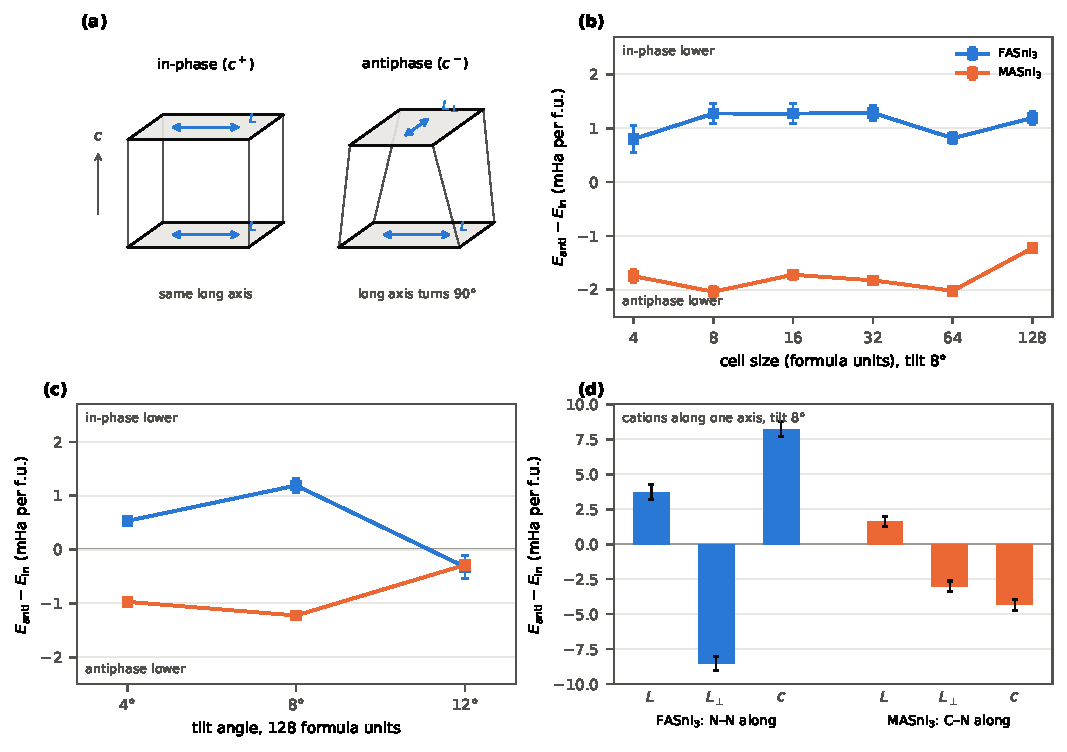
\includegraphics[width=\linewidth]{figures/fig_tilt_scan_si.pdf}
  \caption{\changed{Tilt sense and cation orientation. (a) A tilt about $c$ makes each face of the A-site cage a
  rectangle with long axis $L$; in-phase stacking keeps $L$ at the lower and upper faces, antiphase stacking turns it
  by \ang{90}. (b) Energy of the antiphase relative to the in-phase cell at a tilt of \ang{8} against cell size: mean
  and standard error over 20 to 160 random cation arrangements, cations relaxed with Sn and I fixed. (c) The same
  against the tilt angle in the 128-formula-unit cells. (d) Contribution of cations lying along $L$, $L_\perp$ or
  $c$, from a fit of the energy difference of the 4- and 8-formula-unit cells at \ang{8} to the cation orientations
  (FA: N--N axis; MA: C--N axis). Energies of the \rSCAN{} potential before its final retraining, at the cubic metric of the PBEsol potential (\FASnI{} \SI{6.127}{\angstrom}, \MASnI{} \SI{6.058}{\angstrom}).}}
  \label{fig:si-tilt-scan}
\end{figure}

%% ------------------------------------------------------------
\section{\protect\changed{Results with PBEsol labels}}
\label{si:pbesol}
% moved from the main text (2026-10-29: PBEsol results to the SI)
\changed{This section collects the results on the free crystals obtained with the potentials trained on the PBEsol labels.}

\subsection{Comparison of the two label sets}
\label{sec:si-functional}

% Source: PaperData/paper_figs/fig_functional.py (reads Task4_PhaseTransition/npt_v2_check/xc_compare_v2.json,
% from xc_compare_v2.py); runs: npt_v2_check x2_* and s1p_<864|2304>_*; FinalData/XCselection.
{\changedcolor
We chose between the two label sets by comparing the phase transitions of UrsaMLFF trained on each, with
the D3 parameters and the external pressure of its functional, in two cells per compound, 960 and 2000
atoms for \CsSnI{} and 864 and 2304 atoms for the hybrids, each heated five times at \SI{2}{K/ps}
(protocol in the Supporting Information). Figure~\ref{fig:functional} shows the transition
temperatures on heating and the lattice constants; the two cell sizes agree within the scatter, except
for the $\gamma\leftrightarrow\beta$ transition of \CsSnI{} with PBEsol labels, which lies \SI{46}{K}
higher in the smaller cell. For \CsSnI{} the two functionals err in opposite directions: with PBEsol
labels the transitions lie 31 to \SI{98}{K} above experiment, with \rSCAN{} labels 29 to \SI{51}{K}
below. Both place the orthorhombic-to-tetragonal transition of \MASnI{} far too high (by 88 to
\SI{112}{K}) and its transition to the cubic phase 15 to \SI{31}{K} too high. The loss of tilt order in
\FASnI{} lies within the experimental range with PBEsol labels and 31 to \SI{39}{K} below it with \rSCAN{}
labels. PBEsol is thus closer to experiment for the three transitions into the untilted phase, and
\rSCAN{} for the two $\gamma\leftrightarrow\beta$ transitions; averaged over the five transitions, the
deviations are similar (45 to \SI{51}{K} with PBEsol, 45 to \SI{47}{K} with \rSCAN{}). The lattice
constants separate the functionals clearly: PBEsol with D3 underestimates them by 2.0 to
\SI{2.5}{\percent}, \rSCAN{} with D3 overestimates them by 0.4 to \SI{1.0}{\percent}. Three of the ten
\rSCAN{} runs of \FASnI{} developed molecular defects above \SI{260}{K}, after the loss of tilt order,
and two \rSCAN{} runs of \CsSnI{} in the larger cell two Cs ions in one cage above \SI{520}{K}; these
runs are left out of the averages. The \rSCAN{} training data contain no active-learning structures,
which the PBEsol data needed to keep the hybrid MD free of such defects.

The clamping study of the main text uses the PBEsol labels, because it rests on the transitions into the
untilted phase, which the PBEsol potential places closer to experiment for \CsSnI{}; the price is a lattice compressed
by about \SI{2}{\percent}, and part of the PBEsol agreement comes from a cancellation of errors
(section~\ref{sec:res-free}). The results of the main text on the free crystals use the \rSCAN{} labels.
}

\begin{figure}[htbp]
  \centering
  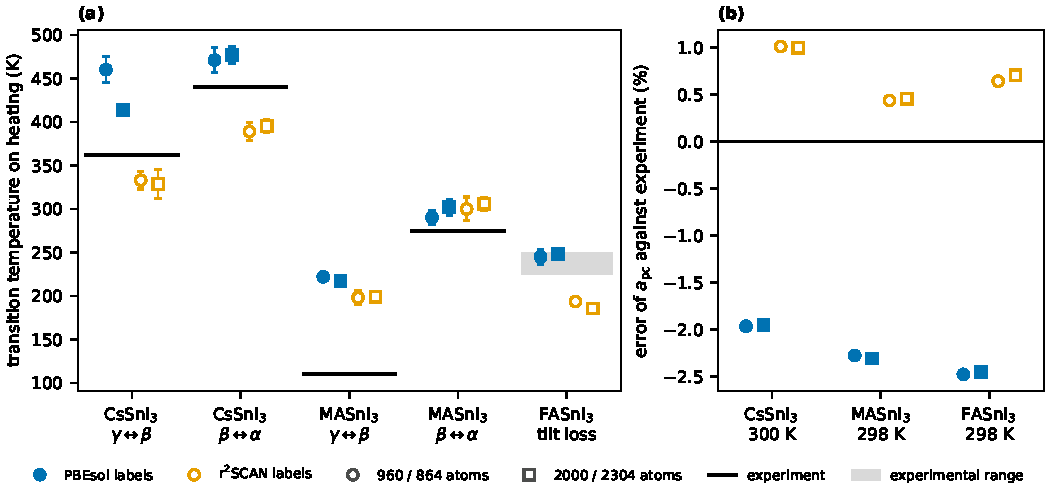
\includegraphics[width=\linewidth]{figures/fig_functional.pdf}
  \caption{Comparison of PBEsol and \rSCAN{} training data. (a) Transition temperatures on heating of
    \changed{UrsaMLFF retrained on PBEsol (filled) and \rSCAN{} labels (open), each with the D3
    parameters and the external pressure of its functional, in cells of 960 and 2000 atoms (\CsSnI{};
    circles and squares) and 864 and 2304 atoms (hybrids)} at \SI{2}{K/ps}, against experiment (black
    lines; grey band: experimental range for
    \FASnI{}).\cite{Chung2012JACS, Yamada2011BCSJ, Takahashi2011Dalton, schueller2018crystal}
    \changed{Mean and standard error of five runs, without the runs with defects (Supporting Information).}
    (b) Error of the pseudo-cubic lattice constant against
    experiment.\cite{Chung2012JACS, Mitzi1995JSSC, schueller2018crystal}}
  \label{fig:functional}
\end{figure}

\subsection{Convergence of the phase transitions with system size}
\label{sec:res-size}

% Sources: Task4_PhaseTransition/size_compare.md (table, generated into tables/tab_size_pbesol.tex);
% paper_figs/fig_size_glazer.py, fig_tiltmaps.py; per-run tilt components checked 2026-10-15.
The transition temperatures of the PBEsol UrsaMLFF were determined in cells of 360 to 4900 atoms
(\CsSnI{}) and 384 to 4800 atoms (hybrids), five runs per cell size and direction, with the
heating and cooling protocol given in the Supporting Information. Table~\ref{tab:size} lists the
transition temperatures, Figure~\ref{fig:size-glazer} the Glazer tilt order along the ramps, and
\changed{Figures~\ref{fig:tilt-pbesol} and~\ref{fig:tilt-r2scan} (section \emph{Octahedral tilt patterns}) the tilt patterns of the phases.}

\paragraph{Phase sequences.}
On heating, \CsSnI{} passes from $a^-a^-c^+$ to $a^0a^0c^+$ to an untilted cubic phase, the tilt
systems of the experimental $Pnma$, $P4/mbm$ and $Pm\bar{3}m$ phases.\cite{Chung2012JACS} \changed{\MASnI{} starts in $a^-a^-c^+$, with an in-phase tilt of \ang{12} about the long axis and antiphase
tilts of about \ang{3.5} about the other two. The antiphase tilts are lost near \SI{217}{K}, leaving
$a^0a^0c^+$, and the in-step stacking of the remaining tilt is lost near \SI{300}{K}. Close to this transition
the tilt about the long axis also forms a layered pattern, with in-phase and antiphase parts of similar size,
in which successive layers tilt by about \ang{11} and \ang{4} (Figure~\ref{fig:big20k}a); the
nearest-neighbour tilt correlation of our transition criterion averages this state to nearly zero although
its tilt persists. The intermediate in-phase state has no experimental counterpart, where the tetragonal
phase has the antiphase tilt $a^0a^0c^-$,\cite{stoumpos2013semiconducting} and marks a limitation of the model
for \MASnI{}. \FASnI{} orders only as $a^0a^0c^+$, the tilt system of its experimental tetragonal
phase,\cite{schueller2018crystal} and loses it at \SI{248}{K}; the orthorhombic phase of \FASnI{} below
\SIrange{125}{150}{K} does not form in our runs.}

% generated by Task4_PhaseTransition/paper_si_tables.py; do not edit
\begin{table}[htbp]
\centering\small
\caption{Transition temperatures (K) against cell size for UrsaMLFF trained on PBEsol labels, with D3 at the constant pressure $P_\mathrm{ext}$, at \SI{2}{K/ps}: mean $\pm$ standard error over the runs with a transition (runs with a transition / runs). Cells are $n_1\times n_2\times n_3$ supercells of the $\sqrt2\times\sqrt2\times2$ setting; the 3600- and 4320-atom cells (even in-plane repeats) were run on cooling only. Noise: the largest tilt correlation (deg) over the hottest \SI{40}{K} of the heating runs, the level the transition criterion has to exceed. The \rSCAN{} values are given in the Supporting Information. \changed{Hybrids: UrsaMLFF retrained on the refined training data; their heating ramps start from structures with the model's \SI{50}{K} cell, their cooling ramps in the cubic phase (starting-cell dependence: Supporting Information).}}
\label{tab:size}
\resizebox{\linewidth}{!}{%
\begin{tabular}{lcccccc}
\toprule
\multicolumn{7}{l}{\CsSnI{}} \\
atoms (cell) & $\gamma\leftrightarrow\beta$ heating & $\gamma\leftrightarrow\beta$ cooling & $\beta\leftrightarrow\alpha$ heating & $\beta\leftrightarrow\alpha$ cooling & & noise \\ \midrule
360 (3$\times$3$\times$2) & 429 $\pm$ 6 (5/5) & 395 $\pm$ 11 (4/5) & 508 $\pm$ 25 (5/5) & 476 $\pm$ 28 (5/5) &  & 2.2 \\
960 (4$\times$4$\times$3) & 407 $\pm$ 8 (5/5) & 360 $\pm$ 34 (5/5) & 456 $\pm$ 10 (5/5) & 416 $\pm$ 20 (5/5) &  & 1.3 \\
2000 (5$\times$5$\times$4) & 411 $\pm$ 7 (5/5) & 327 $\pm$ 13 (5/5) & 462 $\pm$ 17 (5/5) & 377 $\pm$ 13 (5/5) &  & 1.0 \\
2880 (6$\times$6$\times$4) & 411 $\pm$ 5 (5/5) & 352 $\pm$ 16 (5/5) & 449 $\pm$ 7 (5/5) & 375 $\pm$ 18 (5/5) &  & 0.9 \\
3600 (6$\times$6$\times$5) & -- & 314 $\pm$ 16 (5/5) & -- & 332 $\pm$ 16 (5/5) &  & -- \\
4320 (6$\times$6$\times$6) & -- & 302 $\pm$ 22 (5/5) & -- & 334 $\pm$ 13 (5/5) &  & -- \\
4900 (7$\times$7$\times$5) & 407 $\pm$ 3 (5/5) & 314 $\pm$ 8 (5/5) & 461 $\pm$ 9 (5/5) & 341 $\pm$ 4 (5/5) &  & 0.8 \\
\midrule \multicolumn{7}{l}{\MASnI{}} \\
atoms (cell) & $\gamma\leftrightarrow\beta$ heating & $\gamma\leftrightarrow\beta$ cooling & $\beta\leftrightarrow\alpha$ heating & $\beta\leftrightarrow\alpha$ cooling & & noise \\ \midrule
\changed{384 (2$\times$2$\times$2)} & \changed{243 $\pm$ 7 (5/5)} & \changed{188 $\pm$ 28 (4/5)} & \changed{350 $\pm$ 16 (5/5)} & \changed{336 $\pm$ 14 (4/5)} & \changed{} & \changed{2.5} \\
\changed{864 (3$\times$3$\times$2)} & \changed{222 $\pm$ 4 (5/5)} & \changed{170 $\pm$ 0 (2/5)} & \changed{290 $\pm$ 8 (5/5)} & \changed{237 $\pm$ 12 (5/5)} & \changed{} & \changed{1.5} \\
\changed{2304 (4$\times$4$\times$3)} & \changed{217 $\pm$ 3 (5/5)} & \changed{130 (1/5)} & \changed{302 $\pm$ 9 (5/5)} & \changed{211 $\pm$ 13 (4/5)} & \changed{} & \changed{0.7} \\
\changed{4800 (5$\times$5$\times$4)} & \changed{215 $\pm$ 1 (5/5)} & \changed{180 $\pm$ 13 (3/5)} & \changed{281 $\pm$ 7 (5/5)} & \changed{150 $\pm$ 25 (4/5)} & \changed{} & \changed{0.5} \\
\midrule \multicolumn{7}{l}{\FASnI{}: loss of any tilt order} \\
atoms (cell) & heating & cooling & & & & noise \\ \midrule
\changed{384 (2$\times$2$\times$2)} & \changed{259 $\pm$ 9 (5/5)} & \changed{257 $\pm$ 14 (5/5)} & \changed{} & \changed{} & \changed{} & \changed{1.4} \\
\changed{864 (3$\times$3$\times$2)} & \changed{245 $\pm$ 9 (5/5)} & \changed{243 $\pm$ 8 (5/5)} & \changed{} & \changed{} & \changed{} & \changed{0.7} \\
\changed{2304 (4$\times$4$\times$3)} & \changed{248 $\pm$ 6 (5/5)} & \changed{232 $\pm$ 11 (5/5)} & \changed{} & \changed{} & \changed{} & \changed{0.6} \\
\changed{4800 (5$\times$5$\times$4)} & \changed{251 $\pm$ 4 (5/5)} & \changed{220 $\pm$ 9 (5/5)} & \changed{} & \changed{} & \changed{} & \changed{0.5} \\
\bottomrule
\end{tabular}}
\end{table}


% (2026-10-28) the tilt-map figure of the PBEsol heating ramps (fig_tiltmaps) is replaced by
% fig_tiltpatterns_<pbesol|r2scan> in the application section.

\paragraph{Convergence on heating.}
For \CsSnI{} the tilt-order curves of all cells from 960 atoms upward coincide
(Figure~\ref{fig:size-glazer}), and the heating transition temperatures stay within
407--\SI{411}{K} ($\gamma\leftrightarrow\beta$) and 449--\SI{462}{K}
($\beta\leftrightarrow\alpha$) up to 4900 atoms; the 360-atom cell places both transitions
higher and has the largest residual tilt correlation in the cubic phase. \changed{For the hybrids the
384-atom cell is not converged: its residual tilt correlation in the disordered phase, \ang{2.5} for
\MASnI{}, is close to the \ang{3} criterion and places the $\beta\leftrightarrow\alpha$ transition of
\MASnI{} at \SI{350}{K}. From 864 atoms on, every run shows every transition, the residual correlation
falls to \ang{0.5} to \ang{1.5}, and the heating transitions lie at 215--\SI{222}{K}
($\gamma\leftrightarrow\beta$) and 281--\SI{302}{K} ($\beta\leftrightarrow\alpha$) for \MASnI{} and at
245--\SI{251}{K} for \FASnI{}.} Cells of about 2000 atoms (2000 for \CsSnI{}, 2304 for the
hybrids) are therefore the smallest in which the transition statistics are converged, and we use
them for production.

\paragraph{\protect\changed{Starting structure of the hybrid heating runs.}}
\changed{The starting structures of the hybrid heating runs were first built with cells 4--7\,\% (\MASnI{}) and
2--3\,\% (\FASnI{}) longer than the model's \SI{50}{K} cell, which the barostat compresses during the
equilibration at \SI{50}{K}. Crystals prepared this way have the tilt pattern, the cation arrangement and the
energy (within \SI{4e-5}{\hartree} per formula unit) of crystals started in the \SI{50}{K} cell, but carry
about \SI{20}{\percent} more octahedral distortion, with a mean Sn off-centring of 0.113 against
\SI{0.093}{\angstrom}, and keep it on heating. \MASnI{} prepared in the oversized cell loses the in-step
stacking of its tilt at \SI{210 \pm 6}{K} instead of \SI{302 \pm 9}{K} and its second tilted axis at
\SI{152 \pm 2}{K} instead of \SI{217 \pm 3}{K} (2304 atoms), whereas \FASnI{} changes within the error
(\SI{242 \pm 4}{K} against \SI{248 \pm 6}{K}; Table~\ref{tab:si-start-cell}). Every hybrid heating run of
this work therefore starts from the model's \SI{50}{K} cell. Because the nearest-neighbour criterion does not
detect a layered tilt, we also bracketed the equilibrium tilt loss of \MASnI{} with holds of \SI{150}{ps}
at 250, 265 and \SI{280}{K}, each started once from a tilted and once from a cubic crystal (two runs each,
2304 atoms). At \SI{265}{K} both tilted starts keep a layered tilt of about \ang{8} about one axis and one
cubic start forms it; at \SI{280}{K} both cubic starts stay untilted and both tilted starts lose their
coherent tilt within the hold. The equilibrium tilt loss of the model thus lies between 265 and \SI{280}{K},
and the heating transition of the production cell lies about \SI{30}{K} above it, a superheating of the
clean crystal at \SI{2}{K/ps}.}

\paragraph{Cooling.}
On cooling, the transitions occur far below their heating temperatures, and the cooling values
depend on the cell size. The $\beta\leftrightarrow\alpha$ transition of \CsSnI{} falls from
\SI{476}{K} in the 360-atom cell to 332--\SI{341}{K} in the cells of 3600 to 4900 atoms, and
$\gamma\leftrightarrow\beta$ from 395 to 302--\SI{314}{K}, a hysteresis of 60 to \SI{120}{K}
in the cells of 2000 atoms and more against 11 to \SI{14}{K} in experiment.\cite{Chung2012JACS} The state reached on cooling is also
less ordered: at \SI{210}{K} the largest tilt correlation is 5.6 to \ang{11.1} after cooling
against 13.0 to \ang{13.2} after heating, consistent with cooling into several tilt domains that
the larger cells can hold. Cells with odd in-plane repeats cannot hold an in-phase tilt about an
in-plane axis and end less ordered than the even 2880- to 4320-atom cells, but the even cells
give the same cooling transition temperatures as the odd 4900-atom cell, so commensurability is
not the cause. \changed{\FASnI{} orders on cooling in every run, 10 to \SI{25}{K} below its heating
transition. \MASnI{} cools into tilt domains: its local tilt about one axis reaches \ang{7} to \ang{8} at
\SI{150}{K}, but domains of opposite stacking keep its average tilt correlation close to the \ang{3}
criterion, so that its cooling transition temperatures scatter between 150 and \SI{237}{K}; the
18\,432-atom runs show these domains directly (section \emph{Cage and cation angles in 18\,432-atom
cells}). A second tilted axis appears on cooling in one to four of five runs, so that \MASnI{} rarely
reaches its orthorhombic phase, as found for MAPbI$_3$.\cite{Jinnouchi2019PRL, Liang2025ChemMater}} We attribute these effects to the kinetics of nucleating an ordered tilt
pattern at \SI{2}{K/ps}, quote transition temperatures on heating, and measure shifts under
clamping on heating as well.

\begin{figure}[htbp]
  \centering
  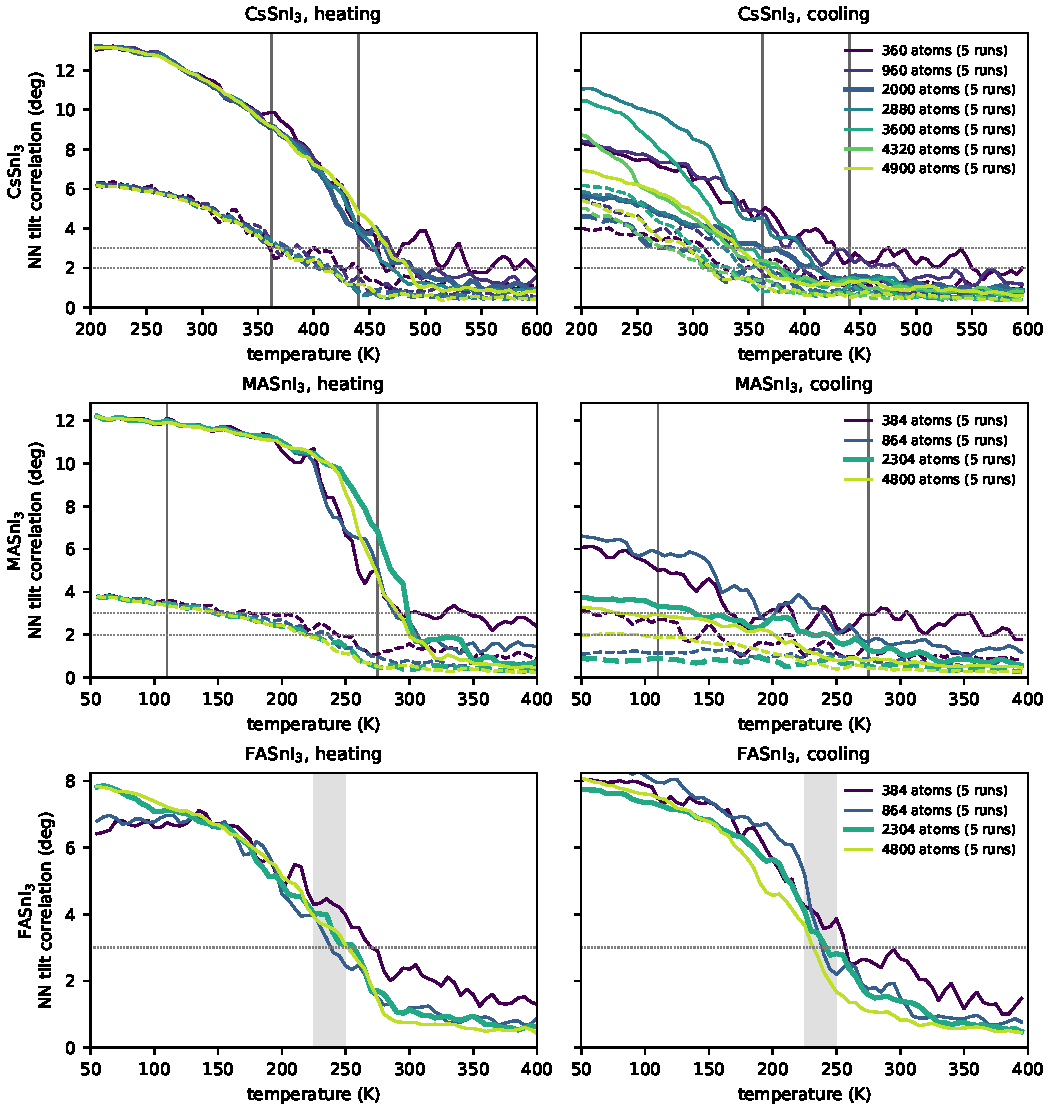
\includegraphics[width=\linewidth]{figures/fig_size_glazer.pdf}
  \caption{Glazer tilt order against temperature for every cell size (PBEsol UrsaMLFF + D3,
    \SI{2}{K/ps}, mean of five runs in \SI{10}{K} windows), on heating (left) and cooling
    (right). Solid lines: largest nearest-neighbour tilt correlation (lost at the transition to the
    cubic phase); dashed lines: second largest (lost when the second tilted axis disappears).
    Dotted lines: the thresholds of the transition criterion; vertical lines and grey band:
    experimental transition temperatures. The production cells (2000 and 2304 atoms) are drawn
    thicker. \changed{Hybrids: retrained UrsaMLFF; heating runs started from the model's \SI{50}{K} cell.}}
  \label{fig:size-glazer}
\end{figure}

\subsection{Transition temperatures compared with experiment}
\label{sec:res-free}

Table~\ref{tab:tc} compares the heating transition temperatures and lattice constants of the
production cells with experiment and with MACE-MH-1 + D3, trained on the same labels.
For \CsSnI{} and \FASnI{} the two potentials agree within \SI{6}{K} and \SI{0.5}{\percent}.
\changed{For \MASnI{}, MACE-MH-1 places both transitions lower; in the same 864-atom cell UrsaMLFF gives
\SI{222 \pm 4}{K} and \SI{290 \pm 8}{K}, against 202 and \SI{237}{K}, so the difference between the
models is largest for the transition to the cubic phase.}

\begin{table}[htbp]
  \centering
  \caption{Transition temperatures on heating and pseudo-cubic lattice constants of the
    free-standing crystals: UrsaMLFF + D3 (PBEsol) in the production cells (\CsSnI{} 2000 atoms,
    \MASnI{} and \FASnI{} 2304 atoms), \SI{2}{K/ps}, mean $\pm$ standard error of five
    runs; MACE-MH-1 + D3 (PBEsol labels) in the cells of the functional comparison (\CsSnI{} 960
    atoms, \MASnI{} and \FASnI{} 864 atoms), \SI{2}{K/ps}, one run; and experiment. \apc{} at \SI{300}{K} (\CsSnI{}) and
    \SI{298}{K} (hybrids). \changed{Hybrids: UrsaMLFF retrained on the refined training data, heating runs
    started from the model's \SI{50}{K} cell.}}
  \label{tab:tc}
  \begin{tabular}{llccc}
    \toprule
    compound & quantity & UrsaMLFF + D3 & MACE-MH-1 + D3 & experiment \\
    \midrule
    \CsSnI{} & $\gamma\leftrightarrow\beta$ (K) & $411 \pm 7$ & 407 & 362\cite{Chung2012JACS} \\
             & $\beta\leftrightarrow\alpha$ (K) & $462 \pm 17$ & 467 & 440\cite{Chung2012JACS} \\
             & \apc{} (\si{\angstrom}) & 6.030 & 6.050 & 6.148\cite{Chung2012JACS} \\
    \MASnI{} & $\gamma\leftrightarrow\beta$ (K) & \changed{$217 \pm 3$} & 202 & $\sim$110\cite{Takahashi2011Dalton, Parrott2016JPCL} \\
             & $\beta\leftrightarrow\alpha$ (K) & \changed{$302 \pm 9$} & 237 & $\sim$275\cite{Yamada2011BCSJ, Takahashi2011Dalton} \\
             & \apc{} (\si{\angstrom}) & \changed{6.103} & 6.133 & 6.2397\cite{Mitzi1995JSSC} \\
    \FASnI{} & loss of tilt order (K) & \changed{$248 \pm 6$} & 247 & 225--250\cite{schueller2018crystal} \\
             & \apc{} (\si{\angstrom}) & \changed{6.160} & 6.189 & 6.316\cite{schueller2018crystal} \\
    \bottomrule
  \end{tabular}
\end{table}

The agreement of the absolute transition temperatures with experiment should not be
over-read. Without D3, the same UrsaMLFF reproduces the lattice constants to within
\SI{1}{\percent} but places the transitions of \CsSnI{} 105 and \SI{143}{K} too low
(\SI{257 \pm 20}{K} and \SI{297 \pm 8}{K} in a 960-atom cell). D3 raises them by about
\SI{160}{K}, mostly by compressing the lattice by about \SI{2}{\percent}: run at the
experimental volume, UrsaMLFF + D3 gives \SI{290 \pm 4}{K} and \SI{340 \pm 7}{K}. The agreement in
Table~\ref{tab:tc} therefore rests partly on a cancellation between the over-binding of D3
and the under-stabilisation of the tilted phases by UrsaMLFF. \changed{Trained on \rSCAN{} labels,
UrsaMLFF gives lattice constants within \SI{1.0}{\percent} of experiment but transition temperatures
of \SI{329 \pm 17}{K} and \SI{395 \pm 7}{K} for \CsSnI{} in the production cell
(Figure~\ref{fig:functional}).} Absolute transition temperatures thus carry an
uncertainty of order \SI{100}{K} between equally defensible models, which is why every
simulation temperature in the clamping study is anchored to the model's own \Tc{}
(section \emph{Effect of process conditions on band-gap deviations}) and why we report only differences.

\subsection{\protect\changed{Cage and cation angles in 18\,432-atom cells}}
\label{sec:res-big}
% Sources: Task4_PhaseTransition/npt_v2_check/big20k (make_big20k.py, make_big20k_r.py, angles20k.py,
% angles_report.py -> angles_tables.md); figure: PaperData/paper_figs/fig_big20k.py.
{\changedcolor
To follow the tilt and cation patterns beyond the production cells, we heated and cooled cells of
18\,432 atoms ($8\times8\times6$, about \SI{7}{nm} across) of both hybrids at \SI{1}{K/ps}, one run per
direction, and analysed the structure averaged over \SI{10}{ps} blocks, the static (time-averaged) and
local (instantaneous) tilts, the Sn--I--Sn angles and the orientations of the cations
(Figure~\ref{fig:big20k}).

\FASnI{} orders as a single in-phase domain that fills the whole cell, on heating and on cooling
(Figure~\ref{fig:big20k}k,l). The tilt of the average structure exceeds \ang{3} below \SI{271}{K} on
heating and below \SI{269}{K} on cooling, so at this size and rate the transition shows no hysteresis. At
\SI{200}{K} the tilt is \ang{6.4} and the in-plane Sn--I--Sn angle of the average structure
\ang{166.6}, against \ang{6.3} and \ang{167.4} measured for the $P4/mbm$ phase,\cite{Kahmann2020ACSEL}
and the apical angle is \ang{175}, against \ang{180}. At \SI{100}{K} the tilt, \ang{7.2}, is the same
in every layer to within \ang{1.1}: the doubling of the $c$ axis with tilts alternating between
\ang{11.6} and \ang{3.8} reported for the low-temperature $P4bm$ phase\cite{Kahmann2020ACSEL} does not
form. On cooling the FA axes concentrate along $\langle100\rangle$ (a fraction of 0.8 at 50 to
\SI{90}{K}) and align with the tilt axis, without nearest-neighbour order of their dipoles.

\MASnI{}, heated from the model's \SI{50}{K} cell, starts in $a^-a^-c^+$ throughout the cell, with an
in-phase tilt of \ang{12} about the long axis that is the same in every layer, antiphase tilts of about
\ang{3.5} about the other two axes, and MA dipoles that lie perpendicular to the long axis and are ordered
antiparallel between nearest neighbours (nearest-neighbour correlation 0.02 at \SI{150}{K}). This cation
order melts between 200 and \SI{280}{K}, and with it the in-step stacking of the tilt: the antiphase tilts
about the short axes are lost near \SI{241}{K}, and from about 265 to \SI{315}{K} the tilt about the long
axis has in-phase and antiphase parts of similar size (\ang{4.9} and \ang{5.7} at \SI{270}{K}), the layered
state of the holds, before the cell becomes cubic near \SI{320}{K} (Figure~\ref{fig:big20k}a). The tilts of
the model are larger than measured: at \SI{200}{K} the in-phase tilt is \ang{11.1} and the in-plane
Sn--I--Sn angle of the average structure \ang{156}, against \ang{8.7} and \ang{162.6} for the $I4cm$
phase,\cite{stoumpos2013semiconducting} and at \SI{140}{K} \ang{11.7} and \ang{155} against \ang{9.3} and
\ang{161.4}.\cite{Takahashi2011Dalton} Cooled from the cubic phase, \MASnI{} splits into tilt domains several
nanometres across with opposite in-phase stacking (Figure~\ref{fig:big20k}j): its local tilt reaches
\ang{7}, but the tilt of the average structure stays below \ang{2}, and its cations do not order
(nearest-neighbour dipole correlation 0.43 at \SI{50}{K}).

The anneals of 18\,432-atom films at the anchored temperatures (\MASnI{} 400 to \SI{327}{K}, \FASnI{} 377
to \SI{304}{K}; free, stress-controlled and rigidly clamped, one run each) reproduce the production cells:
at the end of the hold no film has a tilt above \ang{0.8} about any axis.
}

\begin{figure}[htbp]
  \centering
  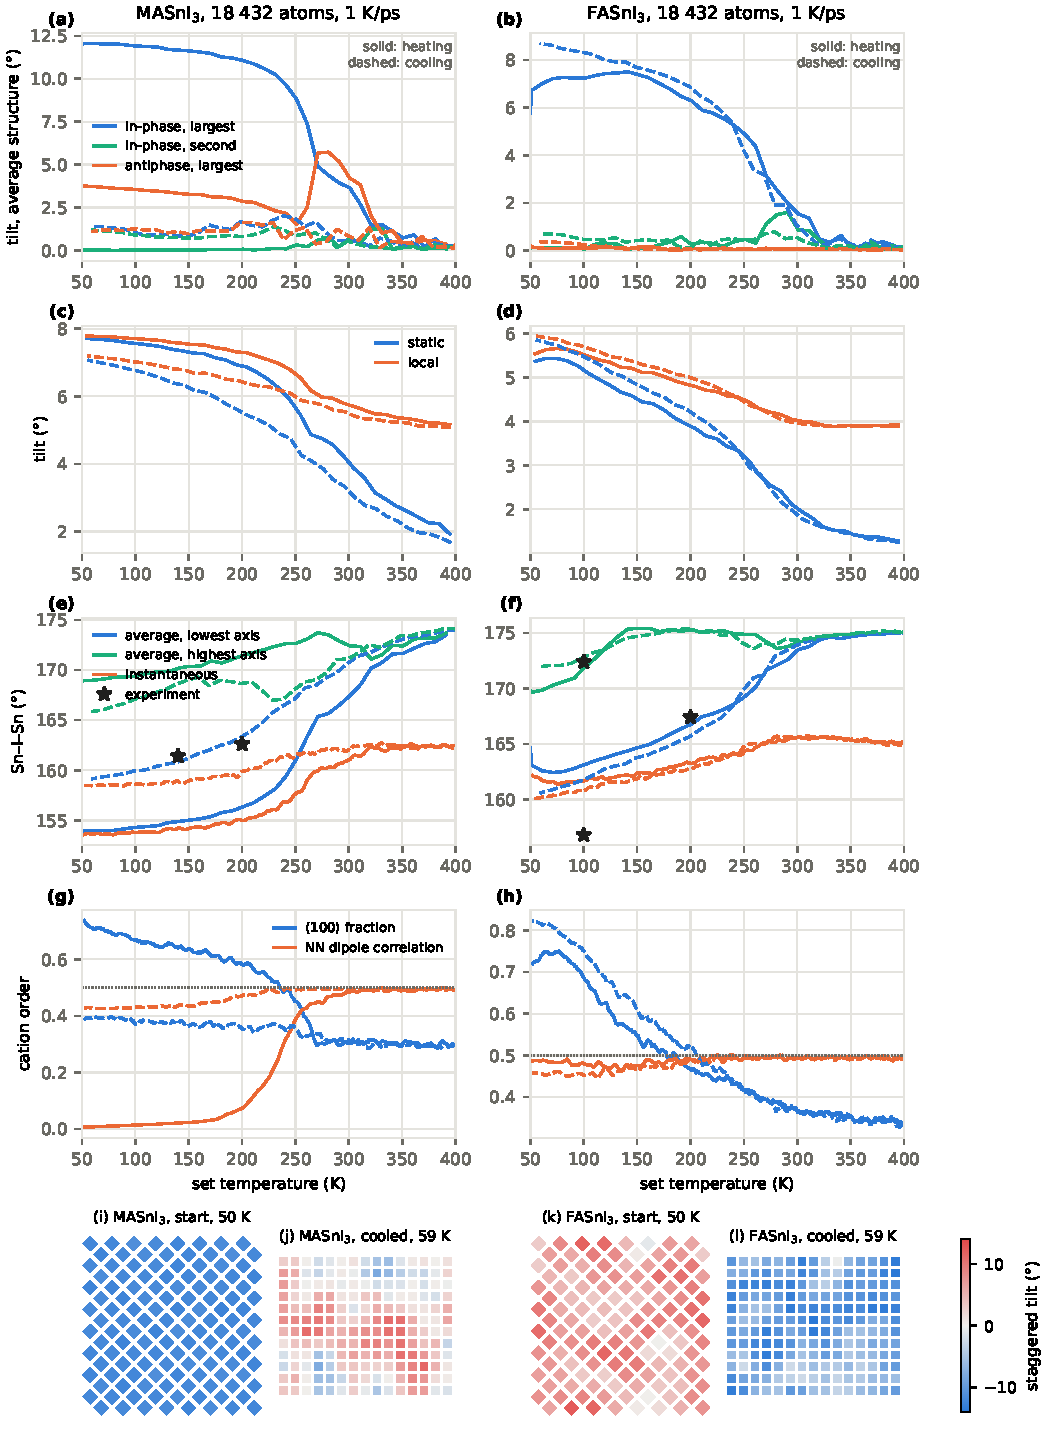
\includegraphics[width=\linewidth]{figures/fig_big20k.pdf}
  \caption{\changed{Cage and cation angles of \MASnI{} (left) and \FASnI{} (right) in 18\,432-atom cells
    (retrained UrsaMLFF + D3, \SI{1}{K/ps}, one run per direction, heating from the model's \SI{50}{K}
    cell; solid heating, dashed cooling).
    (a, b) Tilt amplitudes of the structure averaged over \SI{10}{ps}: largest and second in-phase,
    largest antiphase. (c, d) Static (time-averaged) and local (instantaneous rms) tilt. (e, f) Sn--I--Sn
    angles of the average structure about the most and least bent axis, and the instantaneous angle about
    the most bent axis; stars: experiment (\MASnI{}: $I4cm$ at \SI{200}{K},\cite{stoumpos2013semiconducting}
    $I4/mcm$ at \SI{140}{K};\cite{Takahashi2011Dalton} \FASnI{}: $P4/mbm$ at \SI{200}{K} and the two
    in-plane angles of the alternating layers of $P4bm$ at \SI{100}{K}\cite{Kahmann2020ACSEL}).
    (g, h) Fraction of cation axes nearest to $\langle100\rangle$ and the lowest nearest-neighbour
    dipole correlation (0.5: uncorrelated). (i--l) Tilt about the dominant axis in one layer, with the
    in-phase sign pattern removed, at the lowest temperature of each run: one colour is one domain.}}
  \label{fig:big20k}
\end{figure}

\subsection{\protect\changed{Phase sequences and tilt systems with PBEsol labels}}
\label{sec:si-tilt-pbesol}
{\changedcolor
Figure~\ref{fig:tilt-pbesol} and Tables~\ref{tab:si-tc05-pbesol} and~\ref{tab:si-tilt05-pbesol} give the results of the
protocol of the main text (section~\ref{sec:res-tilt}) with the PBEsol potential; for \MASnI{} two cooling runs were made
in the 18\,432-atom cell. The PBEsol potential reproduces the sequence of \CsSnI{}, $a^0a^0c^+$ followed by $a^-a^-c^+$,
and the in-phase tilt of \FASnI{}, on cooling and on heating. For \MASnI{} two of the three 2304-atom runs form weak
in-phase tilts about one or two axes and the third does not order; both 18\,432-atom runs order only below \SI{185}{K},
one antiphase by about \ang{4.5} and one in-phase by about \ang{7}. PBEsol thus leaves the tilt sense of \MASnI{}
undecided at this rate; at \SI{0.25}{K/ps} all three 2304-atom runs end antiphase. On cooling it places the tilt order of
\MASnI{} at \SI{228 \pm 8}{K} and that of \FASnI{} at \SI{252 \pm 7}{K}. For \CsSnI{} it is closer to experiment than the
\rSCAN{} potential: \SI{413 \pm 17}{K} and \SI{372 \pm 16}{K} against 426 and \SI{351}{K} on cooling, and
\SI{442 \pm 21}{K} against \SI{440}{K} on heating. Tetragonal \FASnI{} tilts by \ang{6.1} and $\gamma$-\CsSnI{} bends its
equatorial and apical Sn--I--Sn bridges by \ang{10.6} and \ang{7.3}; $\beta$-\CsSnI{} tilts in-phase by \ang{7.1}, and at
low temperature the \FASnI{} layers differ by only \ang{1}.

In the static tilt-sense scan (section~\ref{si:tilt-scan}) at \ang{8}, the PBEsol potential
places \FASnI{} lower in-phase by 0.8 to \SI{1.0}{\milli\hartree} per formula unit and \MASnI{} lower antiphase by 0.6 to
\SI{1.2}{\milli\hartree} in cells of 16 to 128 formula units, about half the \rSCAN{} preference for \MASnI{}. The fitted
contribution of a cation lying along $L$ is 2.1 (FA) and \SI{1.3}{\milli\hartree} (MA) per formula unit, and of a cation
standing along $c$ $+6.0$ (FA) and $-\SI{2.6}{\milli\hartree}$ (MA). Where the preference is this weak, the cooling path
decides the sense.
}

\begin{figure}[htbp]
  \centering
  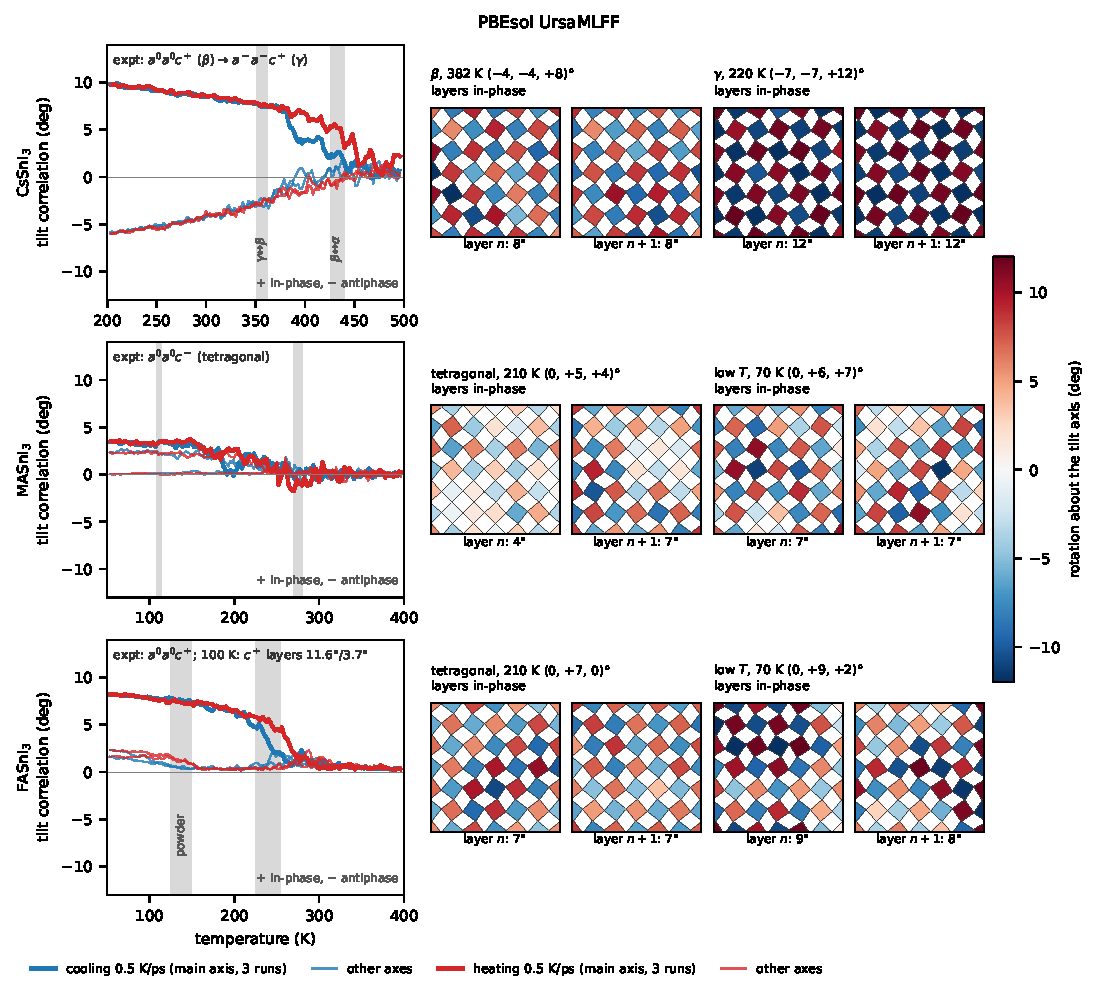
\includegraphics[width=\linewidth]{figures/fig_tiltpatterns_pbesol.pdf}
  \caption{\changed{Tilt patterns with the PBEsol potential (\CsSnI{} 2000 atoms, hybrids 2304); panels as in
    Figure~\ref{fig:tilt-r2scan}, except that every compound is heated back from its cooled crystal.}}
  \label{fig:tilt-pbesol}
\end{figure}

% generated by PaperData/paper_figs/tab_tilt_systems.py; do not edit
\begin{table}[htbp]
\centering\small
\caption{\changed{Transition temperatures (K) at \SI{0.5}{K/ps} with the PBEsol potential: mean $\pm$ standard error of three runs in cells of about 2000 atoms, on cooling from the cubic phase and on heating the cooled crystal, and one cooling run in cells of about 20\,000 atoms. Experiment: heating / cooling. Where not all runs show a transition the mean is over those that do: \MASnI{} $\gamma\leftrightarrow\beta$ and $\beta\leftrightarrow\alpha$: two of the three runs; \FASnI{} second tilted axis: one of the three runs. \dots: no valid run.}}
\label{tab:si-tc05-pbesol}
\begin{tabular}{llcccc}
\toprule
 & & & \multicolumn{2}{c}{2k atoms} & 20k atoms \\
compound & transition & experiment & cooling & heating & cooling \\ \midrule
\changed{\CsSnI{}} & \changed{$\gamma\leftrightarrow\beta$} & \changed{362 / 351\cite{Chung2012JACS}} & \changed{372 $\pm$ 16} & \changed{385 $\pm$ 23} & \changed{385} \\
 & \changed{$\beta\leftrightarrow\alpha$} & \changed{440 / 426\cite{Chung2012JACS}} & \changed{413 $\pm$ 17} & \changed{442 $\pm$ 21} & \changed{425} \\
\changed{\MASnI{}} & \changed{$\gamma\leftrightarrow\beta$} & \changed{114 / 108\cite{Parrott2016JPCL}} & \changed{188 $\pm$ 28} & \changed{188 $\pm$ 42} & \changed{none} \\
 & \changed{$\beta\leftrightarrow\alpha$} & \changed{$\sim$275\cite{Yamada2011BCSJ, Takahashi2011Dalton}} & \changed{228 $\pm$ 8} & \changed{230 $\pm$ 5} & \changed{185} \\
\changed{\FASnI{}} & \changed{second tilted axis} & \changed{125--150 (powder)\cite{schueller2018crystal}} & \changed{100} & \changed{145} & \changed{none} \\
 & \changed{tilt order} & \changed{225--255\cite{schueller2018crystal, Kahmann2020ACSEL}} & \changed{252 $\pm$ 7} & \changed{265 $\pm$ 3} & \changed{250} \\
\bottomrule
\end{tabular}
\end{table}

% generated by PaperData/paper_figs/tab_tilt_systems.py; do not edit
\begin{table}[htbp]
\centering\small
\caption{\changed{Tilt systems and tilt angles (degrees) at \SI{0.5}{K/ps} with the PBEsol potential against the deposited structures (Table~\ref{tab:expt-tilt}), each compared at the same distance below its transition as in experiment (model temperature $T$). Time-averaged structures (\SI{7}{ps}), cooling runs; \CsSnI{} $\beta$: heating runs, middle of the $\beta$ range (on cooling it spans only 5--\SI{50}{K}). Tilt system and angle from the amplitudes averaged over the runs. Single tilt: amplitude about the tilt axis ($+$ in-phase, $-$ antiphase); $Pnma$: equatorial / apical Sn--I--Sn bending $(180^\circ-\theta)/2$; $P4bm$: tilts of the alternating layers. Model amplitudes about each axis from the rotation correlation of neighbouring octahedra along it, insensitive to tilt domains. \MASnI{}: the two runs that tilt.}}
\label{tab:si-tilt05-pbesol}
\resizebox{\linewidth}{!}{%
\begin{tabular}{llllccc}
\toprule
 & \multicolumn{3}{c}{experiment} & \multicolumn{3}{c}{PBEsol} \\
compound & phase, $T$ & tilt system & angle & $T$ (K) & tilt system & angle \\ \midrule
\changed{\CsSnI{}} & \changed{$\beta$ ($P4/mbm$), \SI{380}{K}\cite{Chung2012JACS}} & \changed{$a^0a^0c^+$} & \changed{$+$6.0} & \changed{413} & \changed{$a^0b^-c^+$} & \changed{$+$7.1} \\
 & \changed{$\gamma$ ($Pnma$), \SI{300}{K}\cite{Chung2012JACS}} & \changed{$a^-a^-c^+$} & \changed{11.3 / 6.8} & \changed{321} & \changed{$a^-a^-c^+$} & \changed{10.6 / 7.3} \\
\changed{\MASnI{}} & \changed{tetragonal ($I4cm$), \SI{200}{K}\cite{stoumpos2013semiconducting}} & \changed{$a^0a^0c^-$} & \changed{$-$8.6} & \changed{152} & \changed{$a^0b^+c^+$} & \changed{$+$6.3} \\
 & \changed{tetragonal ($I4/mcm$), \SI{140}{K}\cite{Takahashi2011Dalton}} & \changed{$a^0a^0c^-$} & \changed{$-$9.3} & \changed{92} & \changed{$a^0b^+c^+$} & \changed{$+$6.6} \\
\changed{\FASnI{}} & \changed{tetragonal ($P4/mbm$), \SI{200}{K}\cite{Kahmann2020ACSEL}} & \changed{$a^0a^0c^+$} & \changed{$+$6.3} & \changed{214} & \changed{$a^0a^0c^+$} & \changed{$+$6.1} \\
 & \changed{low $T$ ($P4bm$), \SI{100}{K}\cite{Kahmann2020ACSEL}} & \changed{$c^+$, layers} & \changed{11.6 / 3.7} & \changed{114} & \changed{$a^0a^0c^+$} & \changed{8.8 / 7.8} \\
\bottomrule
\end{tabular}}
\end{table}


%% ------------------------------------------------------------
% Detailed protocol of the application study (moved from the main-text Methods on 2026-10-15, user:
% summary in the Results, details in the SI). Sources as listed in computationalMethodology.tex.
\section{Application protocol: clamping and band gaps}
\label{si:app}

\subsection{Mechanical boundary conditions}
\label{si:brackets-protocol}

\paragraph{Film geometry.}
The $a$ and $b$ axes of the cell are the in-plane directions of a
(001)-oriented film and $c$ is its normal. The stress is
$\sigma = -W/V$, where $W$ is the virial including the kinetic contribution;
positive values are tensile.

\paragraph{Temperature anchoring.}
The absolute transition temperatures of a force field carry its systematic
errors. To place the anneal and the operating point in the same phase and at
the same distance from \Tc{} as in a device, every device temperature $T$ is
mapped onto the model as $T_\mathrm{sim} = T + [\Tc(\mathrm{model}) -
\Tc(\mathrm{expt})]$, using the transition that the anneal-to-operation cooling
path approaches: $\gamma\leftrightarrow\beta$ for \CsSnI{},
$\beta\leftrightarrow\alpha$ for \MASnI{} and the loss of tilt order for
\FASnI{}, each on heating in the production cell. The device temperatures are
the operating temperature (\SI{300}{K}), the damp-heat test (\SI{358}{K}), the
anneal (\SI{373}{K}) and, for \CsSnI{} only, a cubic anneal at \SI{440}{K}. The
shifts are $+49$, \changed{$+27$ and $+4$}~K for \CsSnI{}, \MASnI{} and \FASnI{}, giving
the simulation temperatures of Table~\ref{tab:si-anchored}. A control set at the
unshifted device temperatures (one run per condition) tests the effect of the
anchoring. \changed{The transition temperatures of the hybrids are those of heating runs started from the
model's \SI{50}{K} cell (main text, section \emph{Starting structure of the hybrid heating runs}). The \MASnI{}
shift of $+\SI{27}{K}$ replaces a shift of $-\SI{65}{K}$ obtained from runs started in an oversized cell; the
\MASnI{} runs at 235, 293 and \SI{308}{K} made with that shift are listed in Table~\ref{tab:si-brackets} but not
used in the main text. The \FASnI{} shift was computed from the earlier runs (\SI{242 \pm 4}{K}); the runs from
the \SI{50}{K} cell give \SI{248 \pm 6}{K}, a shift larger by \SI{6}{K}, within the error, so the \FASnI{}
campaigns were kept.}

\begin{table}[htbp]
  \centering
  \caption{Device temperatures and the anchored simulation temperatures
    (K). The shift is $\Tc(\mathrm{model}) - \Tc(\mathrm{expt})$ of the
    anchor transition.}
  \label{tab:si-anchored}
  \begin{tabular}{lcccc}
    \toprule
    & \CsSnI{} & \MASnI{} & \FASnI{} \\
    \midrule
    anchor transition & $\gamma\leftrightarrow\beta$ & $\beta\leftrightarrow\alpha$ & tilt loss \\
    \Tc{} model / expt & 411 / 362 & \changed{302 / 275} & \changed{242$^{b}$ / 238$^{a}$} \\
    shift & $+49$ & \changed{$+27$} & \changed{$+4$} \\
    operation (\SI{300}{K}) & 349 & \changed{327} & \changed{304} \\
    damp heat (\SI{358}{K}) & 407 & \changed{385} & \changed{362} \\
    anneal (\SI{373}{K}) & 422 & \changed{400} & \changed{377} \\
    cubic anneal (\SI{440}{K}) & 489 & -- & -- \\
    \bottomrule
  \end{tabular}
  \begin{flushleft}
    \small $^{a}$ Midpoint of the experimental range \SIrange{225}{250}{K}.\cite{schueller2018crystal}
    \changed{$^{b}$ From the runs started in the oversized cell; \SI{248 \pm 6}{K} from the \SI{50}{K} cell.}
  \end{flushleft}
\end{table}

\paragraph{Three brackets.}
A real film lies between two limits: a free-standing crystal and a crystal
whose in-plane dimensions are fixed by a rigid substrate. We simulate both
limits and one realistic intermediate state, each with three independent runs
at the operating temperature and one at the damp-heat temperature. The free
bracket (ref) applies a constant pressure $P_\mathrm{ext}$ on all three axes.
The stress-controlled bracket (sctl) applies an in-plane tensile stress of
\SI{50}{MPa} ($P_{xx} = P_{yy} = P_\mathrm{ext} - \SI{0.05}{GPa}$) with the
normal free ($P_{zz} = P_\mathrm{ext}$), the residual stress level measured in
perovskite films.\cite{Rolston2018AEM} The rigid clamp with process history
(proc) consists of \SI{50}{ps} of free constant-pressure MD at the anneal
temperature, after which $a$ and $b$ are frozen while $c$ stays free; the cell
is then cooled at \SI{2}{K/ps} to the damp-heat temperature (held
\SI{50}{ps}) and to the operating temperature (held \SI{100}{ps}). The thermal
contraction of the substrate itself is neglected; the residual stress of a
film arises because it is much smaller than that of the
perovskite.\cite{Rolston2018AEM, ref_processing_temp} For \CsSnI{} the same
protocol is also started from the cubic anneal (proccub).
Equilibrium runs start from a heating-ramp frame of the free crystal close to
the target temperature, with the cell set to the five-run mean at that
temperature, and consist of \SI{5}{ps} of constant-volume MD followed by
\SI{150}{ps} at the target condition. The first \SI{50}{ps} of the last stage
are discarded and averages are taken over the remaining frames.

\paragraph{Elastic response.}
Two ladders at the operating temperature give the elastic constants of each
model and the strain dependence of the structure: biaxial strains of $\pm0.25$,
$\pm0.5$, $\pm1$ and $\pm\SI{2}{\percent}$ applied to $a$ and $b$ (frozen,
$c$ free), and hydrostatic pressures of $-0.3$, $-0.15$, $+0.15$, $+0.3$ and
$+\SI{0.6}{GPa}$ relative to $P_\mathrm{ext}$. The biaxial modulus
$Y/(1-\nu)$, Poisson's ratio $\nu$, Young's modulus $Y$ and the bulk modulus
$B$ are fitted to the mean stresses and cells.

\paragraph{Transition temperatures under the clamp.}
Because the model supercools, the shift of a transition under the clamp is
measured on heating. For \CsSnI{}, cells are clamped in-plane at the mean free
cell of the anneal state and heated from the operating temperature at
\SI{2}{K/ps} through both transitions (three runs). The transition temperatures
are determined as for the free ramps, and $\dTc = \Tc(\mathrm{clamped}) -
\Tc(\mathrm{free})$. A $\gamma$-phase cell held under the same clamp at the
operating temperature (\SI{150}{ps}, three runs) provides the clamped $\gamma$
state for the band-gap calculations. Clamped heating runs have so far been made for \CsSnI{} only.

\subsection{Band gaps of the clamped and free ensembles}
\label{si:gaps-protocol}

\paragraph{DFT on production frames.}
Band gaps are computed with the label settings of the main text (\emph{Electronic structure}) on
complete production frames of 2000 or 2304 atoms, so no subcell has to be cut
out of the MD cell. The gap is the lowest unoccupied minus the highest occupied
Kohn--Sham eigenvalue. The supercells sample only the $\Gamma$ point. In the
$\sqrt{2}\times\sqrt{2}\times2$ setting the supercell vectors are
$n_1(1,1,0)$, $n_2(-1,1,0)$ and $n_3(0,0,2)$ in units of \apc{}, so the
pseudo-cubic $R$ point, which carries the band extrema of the cubic phase and
from which those of the tilted phases derive, folds onto $\Gamma$ for every
$n_1$, $n_2$, $n_3$; so does the in-phase tilt vector $M=(\tfrac12,\tfrac12,0)$.
In a pseudo-cubic supercell with an odd number of repeats along an axis, $R$
would instead fold onto the zone boundary, and a $\Gamma$-only gap would be too
large. Each DFT calculation also returns the energy of the frame, which tests
UrsaMLFF in the clamped ensembles.

\paragraph{$\Gamma$-point sampling.}
The folding argument holds for the average structure. A thermal snapshot has
no symmetry beyond the supercell lattice, and disorder could move a band edge
to another point of the supercell zone. Table~\ref{tab:si-gap-kpoints}
collects every DFT calculation of this work that samples more than one
$k$-point. In all 86 static structures and in all 62 MD snapshots of 192 and
240 atoms, both band edges are at $\Gamma$, by at least \SI{213}{meV} for the
valence band and \SI{4}{meV} for the conduction band. The conduction band has
the smaller margin because, without SOC, its minimum at $R$ is threefold
degenerate and includes heavy branches. In the 80-atom fcc-type cell at
\SI{600}{K}, one of two snapshots has its conduction-band minimum off
$\Gamma$, and its $\Gamma$ gap is \SI{11}{meV} too large. Such an error is
bounded by the width of the band-edge bands across the supercell zone, which
falls roughly as the inverse square of the cell length: by a factor of about
five from the 80-atom cell to the hybrid production cells and of about eight
to the \CsSnI{} cells. The $\Gamma$ gap can only overestimate the band-edge
gap, and by similar amounts in clamped and free frames of the same compound,
so the error largely cancels in \dEg{}.

\paragraph{Frame selection.}
Coordinates are never averaged: the gap of the mean structure differs from
the mean gap because averaging removes the tilts that open the gap. Instead, we
select individual frames. For every frame in the averaging window a vector of
structural descriptors is computed: the root-mean-square tilt and the in-phase
and antiphase tilt order about each pseudo-cubic axis, the mean, minimum and
fifth percentile of the Sn--I--Sn angles, the mean, spread and 95th percentile
of the Sn--I bond lengths, the off-centring of Sn in its octahedron, the 95th
percentile of the tilt angles, and for the hybrids the polarisation of the
cation axes, the fractions of cations nearest to $\langle100\rangle$,
$\langle110\rangle$ and $\langle111\rangle$ and the nearest-neighbour
orientational correlation. Within each run the autocorrelation time $\tau$ of
the first principal component of these descriptors defines a spacing
$\Delta = \max(2\tau, \SI{5}{ps})$, and the frames of a bracket are thinned to
at least $\Delta$ apart. The candidates of a bracket are divided into strata,
run $\times$ first or second half of the window, or into clusters when
$k$-means finds a well separated split of the descriptors (silhouette above 0.5
and the smaller cluster above \SI{15}{\percent}), as expected for coexisting
tilt states. Frames are drawn at random within strata with a fixed seed.

\paragraph{Two-level estimator.}
Level~1 isolates the elastic part of the gap change. Six free frames per
material are each computed as they are and after an affine strain to the mean
cell of the stress-controlled bracket, of the rigid clamp, and of the
$\pm\SI{0.3}{GPa}$ hydrostatic runs. Pairing the same configuration cancels
the configurational noise, and the paired differences give the gap change at
fixed internal structure and the deformation potential $\mathrm{d}\Eg/\mathrm{d}\ln V$.
Level~2 compares the ensembles: the mean gap of each bracket is the
stratum-weighted mean $\langle \Eg\rangle = \sum_k w_k m_k$ with the stratum
weights $w_k$ of the candidate pool, and its variance is $\sum_k w_k^2
s_k^2/n_k$; for a stratum with a single frame the spread of the bracket is used.
A pilot of two frames per bracket was planned to set a Neyman
allocation\cite{Neyman1934} of further frames in proportion to $w_k s_k$; its
within-stratum spreads were too uncertain for that, so the three brackets at the
operating temperature were completed to 16 frames each with the frames
distributed over the strata in proportion to $w_k$. Level~1 uses the mean cells
of the first three runs of each bracket, which differ from the eight-run means by
at most \SI{0.08}{\percent} in-plane for the hybrids and \SI{0.16}{\percent}
for the rigid clamp of \CsSnI{}. A ridge regression of the gap on the descriptors was foreseen as a
control variate, $\langle \Eg\rangle \approx \overline{f}_\mathrm{pool} +
\overline{(\Eg - f)}_\mathrm{DFT}$, where $f$ is evaluated on every candidate
frame. On the present frames the frame-averaged descriptors do not predict the
gap (Table~\ref{tab:si-gap-scatter}), so the stratified means are reported
without it. The difference between Level~2 and Level~1 is the part of the gap
change carried by the relaxation of tilts and cation orientations. For each
bracket we report the mean gap shift relative to the free crystal at the same
temperature and the smallest gap of the frames computed, because carriers
collect in the low-gap tail.

{\changedcolor
For \CsSnI{} two further sets complete the estimators. Five Level-1 free
frames are strained to the mean rigid-clamp cell of all eight runs and to the
cell of the clamp set at the cubic anneal; the first gives an elastic part of
\SI{20 \pm 11}{meV}, in agreement with the \SI{19 \pm 7}{meV} obtained at the
three-run cell, and the two cells differ by \SI{-4.3 \pm 0.8}{meV} on the same
frames. One MD frame per run of the free, stress-controlled and rigidly clamped
brackets at the operating temperature (eight each), the three runs of the
$\gamma$ crystal held under the clamp, and two frames each of the cubic-anneal
clamp and of the free crystal at the damp-heat temperature are relaxed with
MACE-MH-1 + D3 (PBEsol labels; D3 as in the production MD) at the fixed mean
cell of the frame's own run over its production window, to a largest force of
\SI{2e-4}{\hartree\per\bohr}. Frames already computed as they are were
preferred, so that 30 of the 31 relaxed frames have the gap of their MD frame
as a partner. Only the atoms move: the relaxed frame keeps the thermal
expansion and the mechanical state of its bracket, and for the rigid clamp the
in-plane cell is the clamp itself. The cell is not relaxed, because the
pressure offset of MACE at the UrsaMLFF cell (\SIrange{0.3}{0.6}{GPa} of
tension in every relaxed frame) would move it away from the ensemble it is
compared with; since every bracket is relaxed in the same way, only differences
between relaxed frames are used. The relaxation keeps the tilt pattern of every
frame, so that the tilt variant of each rigid-clamp run is already present in
its MD frame, and increases the tilt amplitudes by up to about \ang{4}
(Table~\ref{tab:si-gap-relaxed}).\par}

\begin{table}[htbp]
\centering\footnotesize
\caption{Location of the band edges in the DFT calculations of this work that sample more than one $k$-point (PBEsol and \rSCAN{}, perovskite structures; Fermi--Dirac \SI{500}{K}, no SOC; energies in meV). Frames: static, relaxed phases and frozen tilt patterns; MD, snapshots of molecular dynamics. $N$: calculations. At $\Gamma$: calculations with both band edges at $\Gamma$. $\Gamma-\min$: largest difference between the gap at $\Gamma$ and the smallest gap on the mesh. Margins: smallest amount by which $\Gamma$ is the valence-band maximum (VB) and the conduction-band minimum (CB) over the other mesh points; negative when the edge lies elsewhere. The 80-atom cell is the fcc-type supercell with vectors $(0,2,2)$, $(2,0,2)$ and $(2,2,0)$ in units of \apc{}, onto whose $\Gamma$ point $R$ also folds; its snapshots are from \SI{600}{K}.}
\label{tab:si-gap-kpoints}
\begin{tabular}{lrlllrrrr}
\toprule compound & atoms & frames & mesh & functional & $N$ & at $\Gamma$ & $\Gamma-\min$ & margin VB / CB \\ \midrule
\CsSnI{} & 20 & static & 4$\times$4$\times$3 & PBEsol, \rSCAN{} & 76 & 76 & 0 & 406 / 98 \\
\CsSnI{} & 40 & static & 3$\times$3$\times$6 & PBEsol & 3 & 3 & 0 & 335 / 41 \\
\CsSnI{} & 80 & MD & 2$\times$2$\times$2 & \rSCAN{} & 2 & 1 & 11 & 54 / $-$11 \\
\CsSnI{} & 80 & static & 3$\times$3$\times$3 & PBEsol & 3 & 3 & 0 & 336 / 41 \\
\CsSnI{} & 120 & static & 3$\times$3$\times$2 & PBEsol & 4 & 4 & 0 & 336 / 41 \\
\CsSnI{} & 240 & MD & 2$\times$2$\times$1 & PBEsol & 14 & 14 & 0 & 363 / 43 \\
\MASnI{} & 192 & MD & 2$\times$2$\times$3 & PBEsol, \rSCAN{} & 28 & 28 & 0 & 213 / 17 \\
\FASnI{} & 192 & MD & 2$\times$2$\times$3 & PBEsol, \rSCAN{} & 20 & 20 & 0 & 261 / 4 \\
\bottomrule
\end{tabular}
\end{table}


%% ------------------------------------------------------------
\section{Clamping study: all runs}
\label{si:brackets}
\subsection{\protect\changed{Clamped reheating of \CsSnI{}}}
\label{si:clamp-reheat}
% 2026-10-30 (user): moved out of the main text. Runs x21_CS_heat<clamp|free>_s11-13 (npt_v2_check/make_x21_ladders.py),
% onsets from x20_summary.py (criteria of Table tab:phaseid).
{\changedcolor
Whether the substrate constraint moves the transitions of \CsSnI{} is measured on heating, because the model supercools
on cooling. The end states of the free and the clamped films of the main-text protocol (\rSCAN{} potential with D3,
setup~2, three runs each) are heated at \SI{0.25}{K/ps} from the operating temperature to \SI{431}{K} (model
temperatures, \SI{39}{K} below the device scale), the clamped films with $a$ and $b$ still fixed at their anneal values.
The $\gamma\leftrightarrow\beta$ transition does not move: \SI{319}{K} clamped (321, 321, \SI{316}{K}) against
\SI{321}{K} free (316, 321, \SI{326}{K}), $\Delta\Tc = -2 \pm \SI{3}{K}$. The free films lose their last tilt at
$374 \pm \SI{9}{K}$ (381, 386, \SI{356}{K}), whereas all three clamped films keep it up to the top of the ramp, so the
$\beta\leftrightarrow\alpha$ transition rises by at least \SI{57}{K}. Above the anneal temperature the clamped film cannot
expand in the plane, and this in-plane compression relative to the free crystal favours the tilt about the normal. On the
device scale this shift lies above about \SI{410}{K}, outside the operating range, whereas the transition closest to
operation, $\gamma\leftrightarrow\beta$, is unaffected.
}

\subsection{\protect\changed{Strain, tilt and cation orientation}}
\label{si:strain-r2}
% 2026-10-30 (user): r2SCAN only. Data npt_v2_check/ladder_r2_data.py (x20, x21); figure and table paper_figs/fig_ladder_r2.py.
{\changedcolor
Figure~\ref{fig:si-ladder-r2} and Table~\ref{tab:si-ladder-r2} give the response of the octahedral tilt and of the cation
orientation to biaxial in-plane strain and to hydrostatic pressure at the operating temperature (\rSCAN{} potential with D3).
In \CsSnI{} the in-phase tilt about the film normal falls by about \ang{2} per percent of in-plane tension, from \ang{11.8} at
$-\SI{2}{\percent}$ to \ang{6.2} at $+\SI{1}{\percent}$, while the antiphase tilts about the in-plane axes grow; at
$+\SI{2}{\percent}$ the in-phase axis moves into the plane. Hydrostatic compression raises all tilts, by \ang{2.7} per GPa
about the normal, so that per unit change of volume the in-plane strain acts on the tilt about the normal four to five
times more strongly than pressure. \MASnI{} and \FASnI{} stay untilted under tension. A compression of
\SI{0.5}{\percent} induces a weak antiphase tilt about the normal in \MASnI{} (\ang{2.6}), which lies closer to its
transition, whereas \FASnI{} develops only a weak in-phase tilt about an in-plane axis at $-\SI{2}{\percent}$ and
in-phase tilts at $+\SI{0.6}{GPa}$; every induced tilt keeps the sense of the compound.

The cations respond differently. The N--N axes of FA rotate linearly with the strain, towards the film normal and
$\langle100\rangle$ under compression and into the plane under tension ($P_2$ from $+0.105$ at $-\SI{2}{\percent}$ to
$-0.065$ at $+\SI{2}{\percent}$), without a tilt of the framework. The C--N axes of MA turn into the plane under
compression, together with the induced tilt, and do not respond to tension. At the strains of the two substrate setups
(0.2 to \SI{0.4}{\percent}) the tilt of \CsSnI{} about the normal falls from 8.5 to 7.5--\ang{8.1}, the FA axes move
slightly into the plane ($P_2$ lower by 0.005 to 0.02, $f_{100}$ by about 0.008), and the MA orientations do not change.
}

\begin{figure}[htbp]
  \centering
  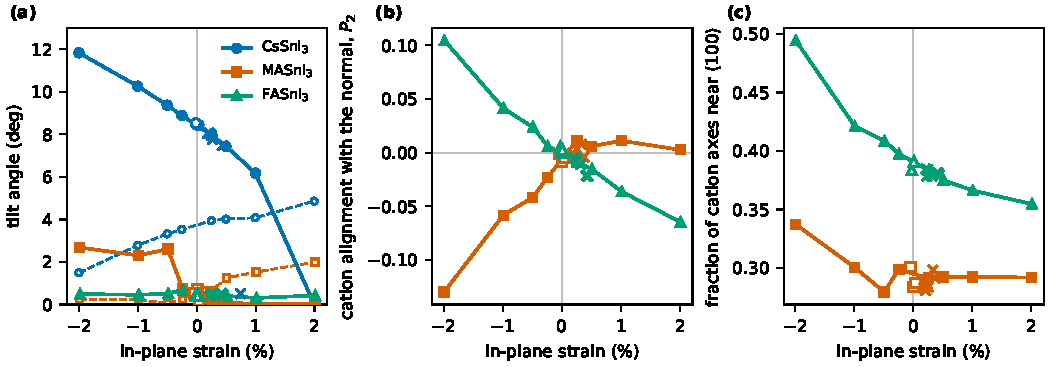
\includegraphics[width=\linewidth]{figures/fig_ladder_r2.pdf}
  \caption{\changed{Response to biaxial in-plane strain at the anchored operating temperature (\rSCAN{} potential with
    D3; ladder: one run per strain, $a$ and $b$ fixed, $c$ free), plotted against the measured in-plane strain. Open
    symbols: the three free films; crosses: the films of setups 1 and 2. (a) Tilt about the film normal (solid; \CsSnI{}
    in-phase, \MASnI{} antiphase, \FASnI{} in-phase) and largest tilt about an in-plane axis (dashed). (b) Alignment of
    the cation axis with the film normal, $P_2 = \langle(3\cos^2\theta-1)/2\rangle$ (MA C--N, FA N--N). (c) Fraction of
    cation axes nearest $\langle100\rangle$.}}
  \label{fig:si-ladder-r2}
\end{figure}

% generated by PaperData/paper_figs/fig_ladder_r2.py; do not edit
\begin{table}[htbp]
\centering\small
\caption{\changed{Octahedral tilt and cation orientation against strain with the \rSCAN{} potential and D3 at the anchored operating temperature: biaxial in-plane strain ($a$ and $b$ fixed, $c$ free) and hydrostatic pressure added to $P_\mathrm{ext}$, one run per point (last \SI{100}{ps}); free films and the films of the two substrate setups, three runs each (\SI{150}{ps} operating hold). Tilt: rotation correlation of neighbouring octahedra (deg; $+$ in-phase, $-$ antiphase) about the film normal $c$ and, for \CsSnI{}, the mean about the in-plane axes. $P_2 = \langle(3\cos^2\theta-1)/2\rangle$: alignment of the cation axis (MA C--N, FA N--N) with the film normal; $f_{100}$: fraction of cation axes nearest $\langle100\rangle$. Run-to-run spread of the free films: tilt \ang{0.1}, $P_2$ 0.004, $f_{100}$ 0.01.}}
\label{tab:si-ladder-r2}
\resizebox{\linewidth}{!}{%
\begin{tabular}{lcccccccc}
\toprule
 & \multicolumn{2}{c}{\CsSnI{} tilt} & \multicolumn{3}{c}{\MASnI{}} & \multicolumn{3}{c}{\FASnI{}} \\
\cmidrule(lr){2-3}\cmidrule(lr){4-6}\cmidrule(lr){7-9}
state & normal & in-plane & tilt & $P_2$ & $f_{100}$ & tilt & $P_2$ & $f_{100}$ \\ \midrule
\changed{biaxial $-$2\,\%} & \changed{$+$11.8} & \changed{$-$1.4} & \changed{$-$2.7} & \changed{$-$0.130} & \changed{0.337} & \changed{$+$0.5} & \changed{$+$0.105} & \changed{0.494} \\
\changed{biaxial $-$1\,\%} & \changed{$+$10.3} & \changed{$-$2.7} & \changed{$-$2.3} & \changed{$-$0.058} & \changed{0.301} & \changed{$+$0.5} & \changed{$+$0.041} & \changed{0.421} \\
\changed{biaxial $-$0.5\,\%} & \changed{$+$9.4} & \changed{$-$3.3} & \changed{$-$2.6} & \changed{$-$0.042} & \changed{0.280} & \changed{$+$0.5} & \changed{$+$0.024} & \changed{0.409} \\
\changed{biaxial $-$0.25\,\%} & \changed{$+$8.9} & \changed{$-$3.5} & \changed{$-$0.7} & \changed{$-$0.023} & \changed{0.299} & \changed{$+$0.7} & \changed{$+$0.006} & \changed{0.397} \\
\changed{free (3 runs)} & \changed{$+$8.5} & \changed{$-$3.6} & \changed{$-$0.5} & \changed{$-$0.005} & \changed{0.291} & \changed{$+$0.4} & \changed{$+$0.003} & \changed{0.389} \\
\changed{biaxial $+$0.25\,\%} & \changed{$+$8.0} & \changed{$-$3.9} & \changed{$-$0.2} & \changed{$+$0.011} & \changed{0.291} & \changed{$+$0.4} & \changed{$-$0.009} & \changed{0.383} \\
\changed{biaxial $+$0.5\,\%} & \changed{$+$7.4} & \changed{$-$4.0} & \changed{$-$0.1} & \changed{$+$0.006} & \changed{0.292} & \changed{$+$0.4} & \changed{$-$0.015} & \changed{0.375} \\
\changed{biaxial $+$1\,\%} & \changed{$+$6.2} & \changed{$-$4.1} & \changed{0.0} & \changed{$+$0.011} & \changed{0.292} & \changed{$+$0.3} & \changed{$-$0.036} & \changed{0.366} \\
\changed{biaxial $+$2\,\%} & \changed{0.0$^b$} & \changed{$+$4.9 / $-$4.6$^b$} & \changed{0.0} & \changed{$+$0.003} & \changed{0.292} & \changed{$+$0.4} & \changed{$-$0.065} & \changed{0.355} \\
\changed{setup 1 (3 runs)} & \changed{$+$8.0$^a$} & \changed{$-$3.8$^a$} & \changed{$-$0.4} & \changed{$-$0.003} & \changed{0.283} & \changed{$+$0.5} & \changed{$-$0.008} & \changed{0.380} \\
\changed{setup 2 (3 runs)} & \changed{$+$7.8} & \changed{$-$3.7} & \changed{$-$0.2} & \changed{$+$0.002} & \changed{0.291} & \changed{$+$0.5} & \changed{$-$0.016} & \changed{0.382} \\
\midrule
\changed{$\Delta P$ $-$0.3\,GPa} & \changed{$+$7.5} & \changed{$-$2.5} & \changed{$-$0.2} & \changed{$+$0.017} & \changed{0.294} & \changed{$+$0.2} & \changed{$-$0.001} & \changed{0.337} \\
\changed{$\Delta P$ $-$0.15\,GPa} & \changed{$+$8.1} & \changed{$-$3.1} & \changed{$-$0.8} & \changed{$-$0.005} & \changed{0.276} & \changed{$+$0.4} & \changed{$-$0.005} & \changed{0.361} \\
\changed{$\Delta P$ $+$0.15\,GPa} & \changed{$+$8.9} & \changed{$-$4.2} & \changed{$-$0.4} & \changed{0.000} & \changed{0.297} & \changed{$+$0.7} & \changed{$+$0.005} & \changed{0.417} \\
\changed{$\Delta P$ $+$0.3\,GPa} & \changed{$+$9.2} & \changed{$-$4.5} & \changed{$-$0.4} & \changed{$-$0.001} & \changed{0.290} & \changed{$+$1.0} & \changed{$+$0.004} & \changed{0.465} \\
\changed{$\Delta P$ $+$0.6\,GPa} & \changed{$+$9.9} & \changed{$-$5.0} & \changed{$+$0.5} & \changed{$+$0.007} & \changed{0.340} & \changed{$+$3.3} & \changed{$-$0.073} & \changed{0.568} \\
\bottomrule
\end{tabular}}
\begin{flushleft}
\small \changed{$^a$ Mean of the two films that keep the in-phase axis along the normal; in the third it moved into the plane. $^b$ The in-phase axis lies in the plane (tilts about the two in-plane axes).}
\end{flushleft}
\end{table}


\subsection{\protect\changed{Clamping study: detailed account}}
\label{si:clamp-detail}
% moved from the main text (2026-10-29, results consolidated); its figures and tables follow this subsection (moved 2026-10-30).
{\changedcolor
A perovskite absorber film is deposited and annealed at an elevated temperature, where it
crystallises on and bonds to its substrate, and is then cooled to its operating temperature
while its in-plane dimensions are restricted by the substrate. The residual stress left by this
history is of order tens of MPa,\cite{Rolston2018AEM, ref_processing_temp} and the corresponding
strain of about \SI{0.5}{\percent}\cite{Zhao2017SciAdv} is comparable to the spontaneous strain of
the structural transitions. \changed{We use the PBEsol force field, whose free-crystal results are given in the Supporting Information,
and PBEsol band gaps, in the converged cells, to} ask how this clamping changes the structure of \CsSnI{}, \MASnI{} and \FASnI{} at their operating
temperature, and how much of the operating band gap it sets. The three compounds sample three
regimes: \CsSnI{}, annealed in its tetragonal phase, crosses the $\gamma\leftrightarrow\beta$
transition on cooling; \MASnI{} operates a few tens of kelvin above its transition; \FASnI{} crosses
no transition between anneal and operation. The protocol, given in full in the Supporting
Information, is summarised here.

All production MD uses the PBEsol UrsaMLFF with D3 at the external pressure $P_\mathrm{ext}$, in
the production cells of 2000 (\CsSnI{}) and 2304 atoms (hybrids), with the $a$ and $b$ axes as the
in-plane directions of a (001)-oriented film\changed{; none of the 88 hybrid runs of the clamping study
contains a molecular defect}. Each device temperature is shifted by the difference
between the model's and the experimental transition temperature of the transition closest to the
anneal-to-operation path (\CsSnI{} $+\SI{49}{K}$, \changed{\MASnI{} $+\SI{27}{K}$, \FASnI{} $+\SI{4}{K}$}),
so that anneal (\SI{373}{K}), damp-heat test (\SI{358}{K}) and operation (\SI{300}{K}) lie in the
same phase and at the same distance from \Tc{} as in a device. \changed{For \MASnI{} the operating point is then \SI{327}{K}, \SI{25}{K} above its heating transition and
about \SI{50}{K} above its equilibrium tilt loss (section \emph{Starting structure of the hybrid heating
runs}); the control set at the unshifted temperatures puts it at \SI{300}{K}, about \SI{25}{K} above the
equilibrium tilt loss.} For \CsSnI{} a cubic anneal
(\SI{440}{K}) is added, and a control set uses the unshifted temperatures. Three mechanical
brackets enclose a real film: a free-standing crystal; a stress-controlled film with an in-plane
tension of \SI{50}{MPa}; and a rigid in-plane clamp set at the anneal, after which the film is
cooled at \SI{2}{K/ps} with its in-plane cell fixed. Each bracket is run three times at the
operating temperature and once at the damp-heat temperature, and each run is held for
\SI{150}{ps}; \changed{five further runs of each operating-temperature bracket enlarge the frame pools of
the band-gap selection}. Biaxial strains of $\pm0.25$ to $\pm\SI{2}{\percent}$ and hydrostatic pressures of
$-0.3$ to $+\SI{0.6}{GPa}$ give the elastic constants of the model and the strain response of the
tilts and of the cation orientations, and clamped cells are heated through the transitions to
obtain $\dTc = \Tc(\mathrm{clamped}) - \Tc(\mathrm{free})$ on the heating branch. Band gaps are
computed with PBEsol DFT at the $\Gamma$ point, onto which the band edges fold for every cell of
this construction (Supporting Information), on complete production frames selected by stratified
sampling in a space of structural descriptors with a fixed seed. A paired estimator, which
computes the same frames as they are and affinely strained to the clamped cells, isolates the
elastic part of the gap change; an ensemble estimator, the stratified mean over the MD frames of
each bracket, gives the total change. \changed{For \CsSnI{}, one MD frame per run of each bracket is also
relaxed at the fixed mean cell of its run; the gaps of these inherent structures carry no thermal
noise, and their difference from the gaps of the MD frames they come from is the thermal part of
the gap.} The DFT energies of the same frames test UrsaMLFF on the clamped ensembles.

We are interested in four quantities: the shift of the transition temperatures under clamping;
the structural response, that is, the tilt amplitudes and patterns and the orientation
distribution of the molecular cations under each bracket, which tests the predicted ordering
\MASnI{} $>$ \FASnI{} $>$ \CsSnI{} ($=0$) of the orientational response; the band-gap shift
between the brackets, split into the elastic part and the part carried by tilts and cation
orientations; and the effect of the anneal temperature as a manufacturing variable.

\paragraph{Elastic response.}

The elastic constants obtained from the strain and pressure ladders at the anchored
operating temperature are listed in Table~\ref{tab:elastic}. \changed{\CsSnI{} is the softest in-plane
and \FASnI{}, about \SI{60}{K} above its tilt transition, the stiffest. With these biaxial moduli an
in-plane stress of \SI{50}{MPa} corresponds to a biaxial strain of about \SI{0.3}{\percent} in \CsSnI{},
\SI{0.19}{\percent} in \MASnI{} and \SI{0.16}{\percent} in \FASnI{}, the range of residual strains measured
in films.\cite{Zhao2017SciAdv} The stress-controlled bracket of \MASnI{} indeed strains it in-plane by
\SI{0.19}{\percent}.}

\paragraph{In-plane strain controls the tilt about the film normal.}

The biaxial ladders show the mechanism by which clamping acts on these films
(Figure~\ref{fig:ladder}a). A tilt about the film normal contracts the in-plane
Sn--Sn distances, so in-plane tension opposes it and in-plane compression favours it. In
\CsSnI{} at \SI{349}{K} the in-phase tilt about the normal falls steadily from
\ang{13.9} at \SI{-2}{\percent} strain to \ang{9.9} in the free crystal and \ang{8.8}
at \SI{+0.5}{\percent}, and collapses between \SI{+0.5}{\percent} and
\SI{+1}{\percent}; at \SI{+2}{\percent} a different pattern with the in-phase axis in the
plane appears. \changed{The two hybrids have no tilt order at their operating points, and compression
induces a tilt about the normal in both, \MASnI{} at half the strain of \FASnI{}. In \MASnI{} at
\SI{327}{K} a compression of \SI{0.5}{\percent} already induces a tilt of \ang{4.3}, with in-phase and
antiphase parts of similar size (the layered pattern), which becomes a pure in-phase tilt of \ang{11.3} at
\SI{-2}{\percent}; a compression of \SI{0.25}{\percent} and every tension leave the normal untilted, and
tension builds a weak antiphase tilt about an in-plane axis, \ang{3.5} at \SI{+2}{\percent}. In \FASnI{} at
\SI{304}{K} compression induces an in-phase tilt about the normal only from \SI{-1}{\percent} on
(\ang{4.6} at \SI{-1}{\percent}, \ang{7.8} at \SI{-2}{\percent}), and tension leaves it untilted.
\MASnI{} operates \SI{25}{K} above its heating transition and \FASnI{} about \SI{60}{K} above its own.}

The orientation of the molecular cations responds much less
(Figure~\ref{fig:ladder}b). \changed{The fraction of FA axes nearest to a pseudo-cubic
$\langle100\rangle$ direction decreases steadily with tension, by 0.07 between \SI{-1}{\percent} and
\SI{+1}{\percent} and by 0.13 across the ladder. The fraction of MA axes near $\langle100\rangle$ stays at
0.30 to 0.32 between \SI{-1}{\percent} and \SI{+2}{\percent} and rises by 0.18 at \SI{-2}{\percent}, where
the in-phase tilt about the normal appears: the MA orientations follow the tilt pattern rather than the
strain.} At the level of these orientation
statistics, the response to strain orders \FASnI{} $>$ \MASnI{}, contrary to our prediction; in
\MASnI{} the strain acts through the octahedral tilt instead.

\paragraph{The three clamping brackets.}

Table~\ref{tab:brackets} summarises the states reached under the three boundary
conditions at the anchored operating temperature. The stress-controlled bracket adds the
intended \SI{50}{MPa} of in-plane tension in all three compounds. It reduces the tilt about
the normal of \CsSnI{} from \ang{9.9} to \ang{9.1} in every run. \changed{Neither hybrid has a tilt about
the normal at its operating point (\MASnI{} \ang{1.5} and \FASnI{} \ang{1.2}, the level of the untilted
crystal), and the tension creates none: in all eight runs of \MASnI{} the tilt about the normal stays at 1.0
to \ang{1.3}, and the tilt about the in-plane axes rises only from 1.5 to \ang{1.7} on average. The cell of
\MASnI{} expands by \SI{0.19}{\percent} in-plane and contracts by \SI{0.14}{\percent} along the normal, a
nearly volumetric strain (volume \SI{+0.23}{\percent}), as that of \FASnI{}.}

The rigid clamp acts differently in each compound. \CsSnI{} is clamped in the $\beta$
phase at the anneal and crosses the $\gamma\leftrightarrow\beta$ transition on cooling. The
three clamped runs end in three different tilt states: one in the free $\gamma$ pattern with
its in-phase axis along the normal, one with the in-phase axis in the plane, and one with
weak, mixed tilts. Their mean in-plane stress equals that of the free crystal, whereas a
$\gamma$ crystal prepared in the free orientation and then held under the same clamp
carries \SI{82}{MPa} of in-plane tension. The clamp thus selects or frustrates tilt
variants rather than straining a single one: the film relieves the clamping stress by
reorganising its tilt pattern. Which variant forms is decided kinetically at \SI{2}{K/ps},
and the odd in-plane repeat of the production cell ($5\times5$) cannot hold an in-phase tilt
about an in-plane axis, which frustrates that variant. Clamped at the cubic anneal
(\SI{440}{K} device, \SI{489}{K} model), \CsSnI{} retains no tilt order at the operating
temperature (all amplitudes below \ang{3}). \changed{\MASnI{} is clamped at \SI{400}{K} and cooled
\SI{73}{K} to its operating point. In all eight runs it stays untilted about the normal (at most
\ang{1.3}) and carries tilts of 1.2 to \ang{2.8} about one in-plane axis and \SI{97}{MPa} of in-plane
tension on average; its cell expands by \SI{0.35}{\percent} in-plane and contracts by \SI{0.24}{\percent}
along the normal. In \FASnI{} neither clamped bracket changes the octahedra (all tilt amplitudes below
\ang{1.6}) or the cation orientations ($f_{\langle100\rangle} = 0.37$ in every bracket). At the unshifted
temperatures (\SI{300}{K}, about \SI{25}{K} above its equilibrium tilt loss), \MASnI{} responds in the same
way (one run per bracket: tilt about the normal at most \ang{1.3}).}

The anchoring of the temperatures is essential to these results. At the unshifted device
temperatures (one run per bracket), \CsSnI{} is \SI{111}{K} below its model
$\gamma\leftrightarrow\beta$ transition at \SI{300}{K}. All brackets, including both
rigid-clamp histories, then end in the free $\gamma$ pattern, and an unanchored simulation
would conclude that clamping has no structural effect on \CsSnI{}.

\paragraph{Transition temperatures under the clamp.}

Heated under the in-plane clamp of the anneal state, \CsSnI{} loses its second tilted axis
at \SI{404 \pm 4}{K} and all tilt order at \SI{448 \pm 19}{K} (three runs; one run keeps
some order to the top of its ramp at \SI{482}{K}), against \SI{411 \pm 7}{K} and
\SI{462 \pm 17}{K} for the free crystal. The shifts, $\dTc = \SI{-7 \pm 8}{K}$ and
\SI{-14 \pm 25}{K}, are zero within their uncertainty. A clamp set by the anneal-state
cell therefore shifts the $\gamma\leftrightarrow\beta$ transition of \CsSnI{} by less than
about \SI{15}{K} on heating, and the shift of the $\beta\leftrightarrow\alpha$ transition is
not resolved. The structural effect of the clamp is on the tilt variants that form on
cooling. Clamped heating runs were made for \CsSnI{} only.

\paragraph{Band-gap shifts.}

\changed{No DFT gaps were computed for \MASnI{} at its anchored operating temperature (\SI{327}{K}); its gaps at \SI{235}{K} are given below.}

\changed{We computed the band gaps of 222 production frames, all of which enter the analysis: 132 frames as
they come from the MD of the brackets, 58 affinely strained frames of the paired estimator, 31
relaxed frames of \CsSnI{} and one frame computed twice (Tables~\ref{tab:gap-elastic}
and~\ref{tab:gap-cs}, and Supporting Information). None of the 100 frames of the hybrids, 50 per
compound\changed{ (those of \MASnI{} from its runs at \SI{235}{K})}, contains a molecular defect (a proton off its cation, a broken C--N bond or a cation out of its
cage).} The same \CsSnI{} frame computed in two independent self-consistent runs
gives gaps that agree to \SI{0.02}{meV}, so the numerical noise of a gap is negligible against the
shifts discussed here.

Table~\ref{tab:gap-elastic} gives the elastic part of the gap change, obtained by straining the
same configurations to the mean cells of the clamped brackets. The gap increases with volume, with
deformation potentials $a_V = \mathrm{d}\Eg/\mathrm{d}\ln V$ of \SI{3.51 \pm 0.12}{eV} for \CsSnI{} and
\changed{\SI{3.49 \pm 0.13}{eV} for \FASnI{}}. This is the sign expected for a valence-band maximum of
antibonding Sn 5s--I 5p character,\cite{huang2013electronic} which rises when the Sn--I bonds are
compressed. Both clamped brackets expand the film in-plane and contract it along the normal, with a net
increase of the volume, and therefore open the gap of \CsSnI{}. At fixed atomic configuration, the
stress-controlled film opens the gap by \SI{18 \pm 6}{meV} and the rigid clamp by \SI{19 \pm 7}{meV} in
\CsSnI{}\changed{, and by \SI{-3 \pm 4}{meV} and \SI{1 \pm 5}{meV} in \FASnI{} (three frames). The clamped
cells of \FASnI{} differ little from the free one (in-plane \SI{+0.14}{\percent} and
\SI{+0.26}{\percent}), and its shifts are zero within their uncertainty, slightly below their volume
parts of 3 and \SI{9}{meV}}. In \CsSnI{} the shift exceeds the volume part by an amount comparable to its
uncertainty.

The ensemble estimator compares the gaps of the MD frames of each bracket (Table~\ref{tab:si-gap-ensemble}).
It contains the elastic part and the relaxation of the tilts and cation orientations that the
clamp induces. With 16 frames per bracket \changed{for \CsSnI{} and 12 for \FASnI{}}, the ensemble
shifts at the operating temperature are \SI{20 \pm 13}{meV} and \changed{\SI{6 \pm 12}{meV}} for
stress-controlled and rigidly clamped \CsSnI{}\changed{, and \SI{-6 \pm 10}{meV} and \SI{-11 \pm 10}{meV} for
\FASnI{}. In \CsSnI{} neither ensemble shift differs from zero by more than 1.6 standard errors, and both
agree with the elastic parts} within about one combined standard error, so the \changed{ensembles alone}
cannot tell whether the relaxation of the structure adds to the elastic shift or removes it\changed{; for
\CsSnI{} the relaxed frames below resolve this. The clamp leaves the gap of \FASnI{} unchanged within about
\SI{20}{meV}; its ensemble shifts agree with the elastic parts within 1.1 combined standard errors
(differences of \SI{-3 \pm 11}{meV} and \SI{-12 \pm 11}{meV}), whereas the volume change alone would open the
gap by 9 and \SI{20}{meV}, and the ensembles lie \SI{15 \pm 10}{meV} and \SI{31 \pm 10}{meV} below it.} The
$\gamma$ phase of \CsSnI{} held under the anneal clamp lies \SI{44 \pm 30}{meV} above the free crystal (two
frames).

{\changedcolor
\paragraph{Distance from the tilt instability.}
How a film responds to a given in-plane strain depends on how far its operating point lies from the
octahedral-tilt instability. \CsSnI{} operates in its tilted $\gamma$ phase: tension reduces its tilt about
the normal and opens its gap, and a clamp that reorganises the tilt variant lowers its inherent gap
(below). The two hybrids operate above their tilt transitions, \MASnI{} by \SI{25}{K} and \FASnI{} by about
\SI{60}{K}. Neither the tension nor the rigid clamp creates a tilt in either, the strain is small and nearly
volumetric, and the gap of \FASnI{} stays within the uncertainty of its volume part. Compression induces a
tilt about the normal in both, in \MASnI{} at half the strain that \FASnI{} needs (\SI{0.5}{\percent}
against \SI{1}{\percent}), so the closer compound to its instability is the one whose tilt a residual
strain changes first. How \MASnI{} responds in its tilted phase just below the transition, where a small
tension moves its tilt from the normal into the plane, is shown in the Supporting Information.
}

The precision of the ensemble estimator is limited by the scatter of the gap from frame to
frame, a standard deviation of \SI{38}{meV} in \CsSnI{} \changed{and \SI{25}{meV} in \FASnI{}} over all
MD frames of a compound (Table~\ref{tab:si-gap-scatter}).
Neither the volume of a frame, nor its mean Sn--I--Sn angle, nor its rms tilt angle predicts its
gap: the leave-one-out errors of linear fits on these descriptors \changed{are at most a quarter below}
the scatter itself. The
band edges of a frame of 2000 atoms thus depend on details of its instantaneous structure that
frame averages do not capture, the descriptor-based control variate does not reduce the variance,
and a standard error of \SI{10}{meV} on the difference of two bracket means requires \changed{29 and 12}
frames per bracket for \CsSnI{} and \FASnI{}.

{\changedcolor
\paragraph{Inherent structures of \CsSnI{}.}
For \CsSnI{} we removed the frame-to-frame scatter by relaxing one MD frame per run of the free,
stress-controlled and rigidly clamped brackets, eight per bracket, together with three
$\gamma$-held, two cubic-anneal and two damp-heat frames (Table~\ref{tab:gap-cs}; every frame in
Table~\ref{tab:si-gap-relaxed}). The atoms were relaxed with MACE-MH-1 + D3, the more accurate of
the two potentials, at the fixed mean cell of the run, so that each relaxed frame keeps the
thermal expansion and the mechanical state of its bracket and differs from its MD frame only by
the thermal displacements. The gaps of the eight relaxed free frames agree to \SI{4}{meV}, against
\SI{38}{meV} for MD frames, and over all relaxed frames the mean Sn--I--Sn angle and the volume
predict the gap to \SI{9}{meV} (leave-one-out), against a spread of \SI{23}{meV}; at fixed volume
the gap closes by \SI{35}{meV} per degree by which the bridges straighten. The scatter of the MD
frames is therefore thermal, and the inherent structures resolve bracket differences of a few meV.

\paragraph{Residual stress in \CsSnI{}.}
In the inherent structures the stress-controlled film lies \SI{26 \pm 2}{meV} above the free
crystal, and the $\gamma$ crystal held under the anneal clamp, which carries \SI{82}{MPa} of
in-plane tension in the MD, lies \SI{20 \pm 2}{meV} above it. Both keep the tilt pattern of the free
crystal. Together with the elastic part at fixed configuration, \SI{18 \pm 6}{meV}, and the shift
of the MD ensembles, \SI{20 \pm 13}{meV}, three estimators built on different frames give an
opening of 18 to \SI{26}{meV} for a residual in-plane tension of \SI{50}{MPa} that leaves the tilt
variant unchanged. This is the effect of residual stress on the band gap of \CsSnI{}.

\paragraph{Processing history of \CsSnI{}.}
The rigid clamp acts through the tilt variant instead. Its eight relaxed frames fall into two
groups. The two runs that kept the in-phase tilt about the normal have gaps \SI{27 \pm 5}{meV}
above the free crystal, like the stress-controlled film. The six runs in which that tilt weakened
or moved into the plane have straighter bridges, with mean Sn--I--Sn angles of 155.4 to
\ang{156.2} against 154.3 to \ang{154.7} in the free crystal and the kept variant, and gaps
\SI{29 \pm 2}{meV} below the free crystal. The change of tilt variant thus lowers the inherent
gap by \SI{56 \pm 5}{meV}, twice the size of the residual-stress effect and of opposite sign.

At the operating temperature thermal motion largely removes this difference. The MD frames lie on
average \SI{71 \pm 11}{meV} above their relaxed structures in the free crystal,
\SI{61 \pm 15}{meV} in the stress-controlled film and \SI{53 \pm 15}{meV} in the kept variant,
but \SI{122 \pm 16}{meV} in the reorganised variant: the weakly tilted structures move furthest
from their inherent structure, and their thermal tilts bend the bridges that the relaxation
straightens. The MD frames of the two variants have mean gaps of 0.618 and \SI{0.632}{eV}, within
their standard errors of 15 to \SI{20}{meV} of the free ensemble at \SI{0.619}{eV}, and the rigid
clamp as a whole shifts the ensemble gap by \SI{6 \pm 12}{meV}. This phonon-induced renormalisation
of the gap\cite{Zacharias2016SDM} depends on the state of the film, so a static structure, relaxed
or averaged, does not give the operating gap of a clamped film, and its difference between states
can differ from the operating one even in sign. For \CsSnI{} clamped at the regular anneal, the
processing history therefore shifts the operating gap by \SI{6 \pm 12}{meV}, consistent with zero,
through a change of tilt variant that lowers the inherent gap and a larger thermal opening of the
reorganised structures that compensates it. The fractions of the two variants, six reorganised
runs of eight, follow from cooling at \SI{2}{K/ps} in a cell whose odd in-plane repeat frustrates
one variant, and are not a prediction for a device; the MD frames of either variant lie within one
standard error of the free ensemble.}

\paragraph{\protect\changed{Anneal temperature and damp heat.}}
The paired estimator also gives the volume part of every bracket difference, $a_V \Delta\ln V$,
from the mean volumes of the ensembles (Table~\ref{tab:si-gap-ensemble}). \changed{The anneal temperature
enters through the in-plane cell that the clamp locks in. Clamped at the regular anneal, \CsSnI{}
at its operating temperature has a mean volume \SI{0.31}{\percent} larger than the free crystal,
and clamped at the cubic anneal \SI{0.57}{\percent} larger, with volume parts of 11 and
\SI{20}{meV}. Straining the same five free frames to the two clamp cells shows that the larger
volume does not open the gap further: the cubic-anneal cell, which also contracts the film more
along the normal (by \SI{1.18}{\percent} against \SI{0.70}{\percent}), opens it by
\SI{4.3 \pm 0.8}{meV} less than the regular-anneal cell, which opens it by
\SI{20 \pm 11}{meV}. The total effect of the cubic anneal, which leaves no tilt order at the
operating temperature, is \SI{-45 \pm 34}{meV} in the ensemble and \SI{4 \pm 16}{meV} in the
inherent structures, with two frames each, and is not resolved.} Heating the free crystals from the
operating to the damp-heat temperature opens the gap by \changed{\SI{53}{meV} in \FASnI{} (one frame at
the damp-heat temperature, against a frame-to-frame scatter of \SI{25}{meV}), of which the thermal
expansion accounts for \SI{27}{meV}}\changed{; in \CsSnI{} the two damp-heat frames give
\SI{-37 \pm 20}{meV} in the ensemble and \SI{18 \pm 32}{meV} in the inherent structures, again
unresolved}.

The DFT energies of the same frames test UrsaMLFF on the production ensembles; forces and
stresses were not computed in these runs. For \CsSnI{} the UrsaMLFF energy lies
\SI{1.1e-4}{\hartree} per atom below DFT, with a spread of \SI{9e-6}{\hartree} per atom over \changed{56}
MD frames of seven brackets, so that energy differences between the ensembles are reproduced to
about \SI{1e-5}{\hartree} per atom. \changed{For \MASnI{} (frames of its runs at \SI{235}{K}) and \FASnI{} the UrsaMLFF energy lies
\SI{3.7e-5}{\hartree} and \SI{2.3e-5}{\hartree} per atom below DFT, with spreads of \SI{4.0e-6}{\hartree}
and \SI{4.4e-6}{\hartree} per atom over 38 MD frames each, below its error on the held-out set
(\SI{6.2e-5}{\hartree} per atom). The offsets of the free, stress-controlled and clamped ensembles differ
by less than \SI{5e-6}{\hartree} per atom (\MASnI{} \SI{-4.0e-5}{}, \SI{-3.6e-5}{} and
\SI{-3.5e-5}{\hartree}; \FASnI{} \SI{-2.5e-5}{}, \SI{-2.3e-5}{} and \SI{-2.1e-5}{\hartree} per atom), so that
energy differences between the hybrid ensembles are reproduced to about \SI{5e-6}{\hartree} per atom.
The clamped hybrid films thus stay within the training data of the force field.}
}

% Floats of the PBEsol clamping study, moved from the main text 2026-10-30 (main text now: r2SCAN setups, sec:res-app).
\begin{table}[htbp]
  \centering
  \caption{Elastic constants at the anchored operating temperature
    (\CsSnI{} \SI{349}{K}, \changed{\MASnI{} \SI{327}{K}, \FASnI{} \SI{304}{K}}), fitted to the
    biaxial-strain and hydrostatic-pressure ladders (one run per point).}
  \label{tab:elastic}
  \begin{tabular}{lcccc}
    \toprule
    compound & $Y/(1-\nu)$ (GPa) & $\nu$ & $Y$ (GPa) & $B$ (GPa) \\
    \midrule
    \CsSnI{} & 15.9 & 0.35 & 10.3 & 14.0 \\
    \changed{\MASnI{}} & \changed{25.7} & \changed{0.29} & \changed{18.2} & \changed{14.7} \\
    \changed{\FASnI{}} & \changed{31.7} & \changed{0.17} & \changed{26.3} & \changed{13.6} \\
    \bottomrule
  \end{tabular}
\end{table}

\begin{figure}[htbp]
  \centering
  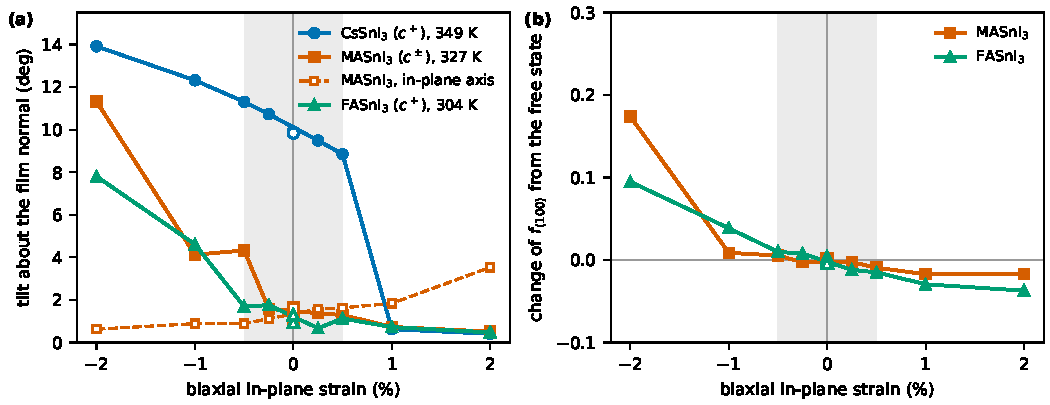
\includegraphics[width=\linewidth]{figures/fig_ladder.pdf}
  \caption{Response to biaxial in-plane strain at the anchored operating temperature
    (filled symbols, one run per strain; $a$ and $b$ fixed, $c$ free). Open symbols: the
    three free runs. Grey band: $\pm\SI{0.5}{\percent}$, the range of measured residual
    strains. (a) Amplitude of the octahedral tilt about the film normal: in-phase ($c^+$)
    for \CsSnI{} and \FASnI{}; \changed{for \MASnI{} the larger of the in-phase and antiphase
    amplitudes, whose pattern changes along the ladder, and (dashed) its largest tilt about an in-plane
    axis}. (b) Change of the fraction
    of cation axes nearest to $\langle100\rangle$, relative to the mean of the free runs
    (\changed{\MASnI{} 0.31, \FASnI{} 0.37}).}
  \label{fig:ladder}
\end{figure}

\begin{table}[htbp]
  \centering
  \caption{States at the anchored operating temperature under the three brackets. $\Delta
    \sigma_\parallel$: mean in-plane stress relative to the free runs (MPa, tensile
    positive). Tilt: amplitude about the film normal (deg; \CsSnI{} and \FASnI{} in-phase,
    \changed{\MASnI{} the larger of the in-phase and antiphase amplitudes}), mean and individual runs.
    $f_{\langle100\rangle}$: fraction of cation axes nearest to $\langle100\rangle$. Three runs per entry
    \changed{(seeds 11 to 13; the hybrids have five more runs per bracket, described in the text)}.}
  \label{tab:brackets}
  \begin{tabular}{llccc}
    \toprule
    compound & bracket & $\Delta\sigma_\parallel$ & tilt (runs) & $f_{\langle100\rangle}$ \\
    \midrule
    \CsSnI{} & free & 0 & 9.9 (9.9, 9.8, 9.8) & -- \\
             & stress-controlled & $+50$ & 9.1 (9.2, 9.1, 9.0) & -- \\
             & rigid clamp & $0$ & 4.1 (1.6, 8.6, 2.2) & -- \\
             & $\gamma$ held under clamp & $+82$ & 7.9 (7.8, 7.8, 8.1) & -- \\
    \changed{\MASnI{}} & \changed{free} & \changed{0} & \changed{1.2 (1.0, 1.6, 1.1)} & \changed{0.31} \\
             & \changed{stress-controlled} & \changed{$+51$} & \changed{1.1 (1.0, 1.2, 1.1)} & \changed{0.30} \\
             & \changed{rigid clamp} & \changed{$+70$} & \changed{1.1 (1.1, 0.8, 1.3)} & \changed{0.30} \\
    \changed{\FASnI{}} & \changed{free} & \changed{0} & \changed{1.2 (0.9, 1.3, 1.3)} & \changed{0.37} \\
             & \changed{stress-controlled} & \changed{$+49$} & \changed{1.3 (1.3, 1.6, 1.0)} & \changed{0.37} \\
             & \changed{rigid clamp} & \changed{$+92$} & \changed{0.8 (0.5, 0.9, 1.0)} & \changed{0.37} \\
    \bottomrule
  \end{tabular}
\end{table}

\begin{table}[htbp]
\centering\small
\caption{Elastic part of the gap change under clamping (PBEsol, no SOC). Free frames at the operating temperature are computed as they are and after an affine strain to the mean cell of the stress-controlled bracket and of the rigid clamp. $\dEg$: mean paired change $\pm$ standard error over $n$ frames (meV). $\Delta\ln V$: mean volume change (\%). $a_V\Delta\ln V$: the part of $\dEg$ accounted for by the volume change alone (meV), with the deformation potential $a_V = \mathrm{d}\Eg/\mathrm{d}\ln V$ from the same frames strained to the mean cells of the $\pm\SI{0.3}{GPa}$ hydrostatic runs.}
\label{tab:gap-elastic}
\begin{tabular}{lcccccccc}
\toprule
 & & \multicolumn{3}{c}{stress-controlled} & \multicolumn{3}{c}{rigid clamp} & \\
\cmidrule(lr){3-5}\cmidrule(lr){6-8}
compound & $n$ & $\dEg$ & $\Delta\ln V$ & $a_V\Delta\ln V$ & $\dEg$ & $\Delta\ln V$ & $a_V\Delta\ln V$ & $a_V$ (eV) \\ \midrule
\CsSnI{} & 6 & 18 $\pm$ 6 & $+$0.32 & $+$11.2 & 19 $\pm$ 7 & $+$0.25 & $+$8.8 & 3.51 $\pm$ 0.12 \\
\changed{\FASnI{}} & \changed{3} & \changed{$-$3 $\pm$ 4} & \changed{$+$0.09} & \changed{$+$3.2} & \changed{1 $\pm$ 5} & \changed{$+$0.27} & \changed{$+$9.4} & \changed{3.49 $\pm$ 0.13} \\
\bottomrule
\end{tabular}
\begin{flushleft}
\small \changed{\MASnI{}: no DFT gaps at its anchored operating temperature (\SI{327}{K}); the frames computed at \SI{235}{K}, below its tilt transition, are reported in the Supporting Information.}
\end{flushleft}
\end{table}


\begin{table}[htbp]
\centering\small
\changedcolor
\caption{\protect\changed{Band-gap change of \CsSnI{} against the free crystal at the anchored operating temperature (PBEsol at $\Gamma$, no SOC; meV, mean $\pm$ standard error, $n$ frames). Elastic: free MD frames computed as they are and affinely strained to the mean cell of the bracket (for the rigid clamps, the mean of all eight runs). Relaxed: MD frames relaxed at the fixed mean cell of their run, one per run (inherent structures); the free crystal has $\langle\Eg\rangle = \SI{0.538}{eV}$ with a spread of \SI{4}{meV} over eight runs. Thermal: $\Eg$(MD frame) $-$ $\Eg$(the same frame relaxed), averaged over the pairs. MD ensemble: stratified mean of the frames as they come from the MD (Table~\ref{tab:si-gap-ensemble}). The rigid-clamp runs are split by the in-phase tilt about the film normal after relaxation: kept above \ang{10}, as in every free, stress-controlled and $\gamma$-held frame, or weakened and reorganised.}}
\label{tab:gap-cs}
\begin{tabular}{lcccccc}
\toprule
 & \multicolumn{1}{c}{elastic} & \multicolumn{2}{c}{relaxed} & thermal & \multicolumn{2}{c}{MD ensemble} \\
\cmidrule(lr){2-2}\cmidrule(lr){3-4}\cmidrule(lr){5-5}\cmidrule(lr){6-7}
state & $\dEg$ ($n$) & $n$ & $\dEg$ & & $n$ & $\dEg$ \\ \midrule
free & -- & 8 & 0 & 71 $\pm$ 11 & 16 & 0 \\
stress-controlled (\SI{50}{MPa}) & 18 $\pm$ 6 (6) & 8 & 26 $\pm$ 2 & 61 $\pm$ 15 & 16 & 20 $\pm$ 13 \\
rigid clamp, all runs & 20 $\pm$ 11 (5) & 8 & $-$15 $\pm$ 9 & 105 $\pm$ 16 & 16 & 6 $\pm$ 12 \\
\quad tilt about the normal kept & -- & 2 & 27 $\pm$ 5 & 53 $\pm$ 15 & -- & -- \\
\quad tilt reorganised & -- & 6 & $-$29 $\pm$ 2 & 122 $\pm$ 16 & -- & -- \\
$\gamma$ held under clamp$^{a}$ & -- & 3 & 20 $\pm$ 2 & 106 $\pm$ 28 & 2 & 44 $\pm$ 30 \\
rigid clamp, cubic anneal & 16 $\pm$ 11 (5) & 2 & 4 $\pm$ 16 & 33 $\pm$ 49 & 2 & $-$45 $\pm$ 34 \\
free, \SI{358}{K}$^{b}$ & -- & 2 & 18 $\pm$ 32 & 26 $\pm$ 50 & 2 & $-$37 $\pm$ 20 \\
\bottomrule
\end{tabular}
\begin{flushleft}
\small $^{a}$ Thermal part from two pairs (one relaxed frame has no MD partner). $^{b}$ Damp-heat device temperature; differences from the free crystal at the operating temperature.
\end{flushleft}
\end{table}



% Source: Task4_PhaseTransition/stress_summary.md, stress_A_*/analysis/*.npz (generated table).
Table~\ref{tab:si-brackets} lists the production-window averages of every run of the clamping study
with UrsaMLFF (PBEsol, D3). Each run is named by compound, protocol and seed. The protocols are: ref, the
free crystal; sctl, the stress-controlled film with an in-plane tension of \SI{50}{MPa}; proc, the
rigid in-plane clamp set at the anneal and cooled to the operating temperature; proccub (\CsSnI{} only),
the same clamp set at the cubic anneal; ref358 and sctl358, the free and stress-controlled states at
the damp-heat temperature; clampgamma (\CsSnI{} only), the $\gamma$ phase held under the anneal clamp;
biax\_mXXX and biax\_pXXX, biaxial strains of $-$XXX and $+$XXX hundredths of a percent with $a$ and
$b$ fixed and $c$ free; and hyd\_mXXX and hyd\_pXXX, hydrostatic pressures of $-$XXX and $+$XXX
hundredths of a GPa relative to $P_\mathrm{ext}$. Runs marked (nom) belong to the control set at the
unshifted device temperatures. The free axes of every run sit at the target stress $-P_\mathrm{ext}$, so
stresses relative to the free crystal are obtained by subtracting the free-crystal values.
\changed{With the retrained UrsaMLFF every hybrid run completed without a molecular defect.}

\changed{\paragraph{\MASnI{} at the anchor before the correction of the starting cell.} The \MASnI{} runs at 235,
293 and \SI{308}{K} (operation, damp heat and anneal) used the shift of $-\SI{65}{K}$ derived from heating
runs started in an oversized cell. At \SI{235}{K} \MASnI{} lies about \SI{35}{K} below the equilibrium tilt
loss of the model, in a layered tilt about the normal (two of three free runs at \ang{6.1} and \ang{5.8}, one
at \ang{2.4}). There a biaxial strain between \SI{-0.25}{\percent} and \SI{+0.25}{\percent} removes the tilt
about the normal, and tension moves it into the plane (an antiphase tilt of \ang{5.9} at \SI{+1}{\percent});
the rigid clamp removes it in all eight runs and the tension of \SI{45}{MPa} in five of eight, with a
tetragonal cell (in-plane $+0.6$, normal $\SI{-1.0}{\percent}$, volume $\SI{+0.2}{\percent}$). DFT on these
frames gives an elastic gap shift of \SI{58 \pm 18}{meV} for both clamped cells and ensemble shifts of
\SI{29 \pm 13}{meV} (tension) and \SI{40 \pm 12}{meV} (clamp); at the same stress the frames whose tilt left the
normal have a gap \SI{46 \pm 13}{meV} above those whose tilt stayed (Table~\ref{tab:si-gap-ensemble}). These
runs show how \MASnI{} responds in its tilted phase near the transition; they are not the anchored operating
state and are not used in the main text.}

\begin{landscape}
\scriptsize
\begin{longtable}{llrrrrrrrrrc}
\caption{Every run of the clamping study: production-window means. $T$: set temperature (K); $a$, $b$, $c$: cell (\si{\angstrom}); $\sigma$: stress (GPa, tensile positive; the free axes sit at $-P_\mathrm{ext}$); tilt amplitudes (deg) in-phase ($+$) about the normal and antiphase ($-$) about $x$, $y$, $z$; $f_{100}$: fraction of cation axes nearest $\langle100\rangle$. Campaign suffix nom: unanchored device temperatures. \changed{\MASnI{} runs at 235 and \SI{293}{K}: the anchor before the correction of the starting cell; at 327 and \SI{385}{K}: the corrected anchor used in the main text.}}\label{tab:si-brackets}\\
\toprule run & $T$ & $a$ & $b$ & $c$ & $\sigma_{xx}$ & $\sigma_{yy}$ & $\sigma_{zz}$ & $+z$ & $-x$ & $-y$ & $-z$ / $f_{100}$ \\ \midrule \endfirsthead
\toprule run & $T$ & $a$ & $b$ & $c$ & $\sigma_{xx}$ & $\sigma_{yy}$ & $\sigma_{zz}$ & $+z$ & $-x$ & $-y$ & $-z$ / $f_{100}$ \\ \midrule \endhead
\bottomrule \endfoot
CsSnI3\_ref\_s11 & 349 & 42.763 & 42.337 & 48.665 & 0.064 & 0.055 & 0.049 & 9.9 & 5.1 & 5.1 & 0.3 \\
CsSnI3\_sctl\_s11 & 349 & 42.816 & 42.487 & 48.559 & 0.114 & 0.105 & 0.049 & 9.2 & 5.3 & 5.3 & 0.3 \\
CsSnI3\_proc\_s11 & 349 & 42.752 & 42.784 & 48.225 & 0.030 & 0.037 & 0.058 & 1.6 & 5.9 & 0.7 & 1.3 \\
CsSnI3\_ref\_s12 & 349 & 42.652 & 42.449 & 48.695 & 0.053 & 0.068 & 0.060 & 9.8 & 4.9 & 4.8 & 0.3 \\
CsSnI3\_sctl\_s12 & 349 & 42.712 & 42.590 & 48.592 & 0.102 & 0.117 & 0.061 & 9.1 & 5.0 & 5.1 & 0.3 \\
CsSnI3\_proc\_s12 & 349 & 42.709 & 42.510 & 48.652 & 0.086 & 0.080 & 0.062 & 8.6 & 4.3 & 3.6 & 0.7 \\
CsSnI3\_ref\_s13 & 349 & 42.828 & 42.305 & 48.661 & 0.085 & 0.061 & 0.055 & 9.8 & 5.1 & 5.1 & 0.3 \\
CsSnI3\_sctl\_s13 & 349 & 42.873 & 42.479 & 48.550 & 0.134 & 0.110 & 0.055 & 9.0 & 5.3 & 5.0 & 0.3 \\
CsSnI3\_proc\_s13 & 349 & 42.769 & 42.724 & 48.390 & 0.079 & 0.070 & 0.069 & 2.2 & 1.2 & 2.5 & 1.5 \\
CsSnI3\_ref358\_s11 & 407 & 42.803 & 42.744 & 48.544 & 0.065 & 0.054 & 0.047 & 4.4 & 0.7 & 1.6 & 0.8 \\
CsSnI3\_sctl358\_s11 & 407 & 42.979 & 42.925 & 48.243 & 0.114 & 0.103 & 0.047 & 0.8 & 1.5 & 3.1 & 0.9 \\
CsSnI3\_proccub\_s11 & 349 & 42.897 & 42.960 & 48.109 & 0.130 & 0.145 & 0.068 & 0.9 & 0.9 & 0.8 & 1.0 \\
CsSnI3\_biax\_m200\_s11 & 349 & 41.992 & 41.361 & 49.369 & -0.534 & -0.483 & 0.052 & 13.9 & 3.9 & 4.0 & 0.1 \\
CsSnI3\_biax\_m100\_s11 & 349 & 42.420 & 41.783 & 49.057 & -0.207 & -0.199 & 0.050 & 12.3 & 4.3 & 4.4 & 0.2 \\
CsSnI3\_biax\_m050\_s11 & 349 & 42.635 & 41.994 & 48.879 & -0.069 & -0.077 & 0.050 & 11.3 & 4.7 & 4.8 & 0.2 \\
CsSnI3\_biax\_m025\_s11 & 349 & 42.742 & 42.099 & 48.782 & 0.006 & -0.016 & 0.047 & 10.7 & 5.0 & 4.9 & 0.2 \\
CsSnI3\_biax\_p025\_s11 & 349 & 42.956 & 42.310 & 48.583 & 0.134 & 0.083 & 0.046 & 9.5 & 5.3 & 5.5 & 0.2 \\
CsSnI3\_biax\_p050\_s11 & 349 & 43.063 & 42.416 & 48.489 & 0.200 & 0.137 & 0.049 & 8.8 & 5.6 & 5.5 & 0.2 \\
CsSnI3\_biax\_p100\_s11 & 349 & 43.277 & 42.627 & 48.044 & 0.212 & 0.079 & 0.044 & 0.6 & 0.8 & 1.9 & 1.1 \\
CsSnI3\_biax\_p200\_s11 & 349 & 43.706 & 43.049 & 47.760 & 0.542 & 0.416 & 0.051 & 0.4 & 6.7 & 1.5 & 0.4 \\
CsSnI3\_hyd\_m030\_s11 & 349 & 42.980 & 42.946 & 48.889 & 0.364 & 0.355 & 0.349 & 6.4 & 2.7 & 3.0 & 0.9 \\
CsSnI3\_hyd\_m015\_s11 & 349 & 42.862 & 42.597 & 48.803 & 0.214 & 0.205 & 0.199 & 9.2 & 4.4 & 4.5 & 0.3 \\
CsSnI3\_hyd\_p015\_s11 & 349 & 42.680 & 42.093 & 48.525 & -0.086 & -0.096 & -0.101 & 10.4 & 5.4 & 5.5 & 0.2 \\
CsSnI3\_hyd\_p030\_s11 & 349 & 42.626 & 41.816 & 48.413 & -0.236 & -0.246 & -0.251 & 11.1 & 5.9 & 5.8 & 0.2 \\
CsSnI3\_hyd\_p060\_s11 & 349 & 42.663 & 41.102 & 48.244 & -0.535 & -0.546 & -0.552 & 12.5 & 6.4 & 6.5 & 0.2 \\
CsSnI3\_ref\_s11 (nom) & 300 & 42.942 & 41.882 & 48.676 & 0.065 & 0.056 & 0.050 & 11.3 & 5.9 & 5.9 & 0.2 \\
CsSnI3\_sctl\_s11 (nom) & 300 & 42.966 & 42.064 & 48.569 & 0.115 & 0.105 & 0.050 & 10.7 & 6.1 & 6.1 & 0.2 \\
CsSnI3\_proc\_s11 (nom) & 300 & 42.601 & 42.549 & 48.531 & 0.089 & 0.160 & 0.057 & 9.9 & 5.8 & 5.8 & 0.2 \\
CsSnI3\_ref358\_s11 (nom) & 358 & 42.737 & 42.429 & 48.657 & 0.065 & 0.055 & 0.049 & 9.5 & 4.8 & 4.7 & 0.3 \\
CsSnI3\_sctl358\_s11 (nom) & 358 & 42.803 & 42.547 & 48.564 & 0.114 & 0.105 & 0.048 & 8.9 & 5.1 & 5.1 & 0.3 \\
CsSnI3\_proccub\_s11 (nom) & 300 & 42.730 & 42.766 & 48.372 & 0.234 & 0.190 & 0.067 & 8.7 & 6.1 & 6.1 & 0.2 \\
CsSnI3\_clampheat\_s11 & 465 & 42.760 & 42.747 & 48.718 & -0.007 & -0.009 & 0.076 & 1.5 & 0.7 & 0.8 & 2.9 \\
CsSnI3\_clampgamma\_s11 & 349 & 42.760 & 42.747 & 48.446 & 0.147 & 0.136 & 0.048 & 7.8 & 4.9 & 5.2 & 0.3 \\
CsSnI3\_clampheat\_s12 & 465 & 42.760 & 42.747 & 48.760 & 0.005 & -0.001 & 0.082 & 5.5 & 1.2 & 0.9 & 1.0 \\
CsSnI3\_clampgamma\_s12 & 349 & 42.760 & 42.747 & 48.465 & 0.138 & 0.153 & 0.060 & 7.8 & 5.4 & 4.6 & 0.3 \\
CsSnI3\_clampheat\_s13 & 465 & 42.760 & 42.747 & 48.703 & -0.008 & -0.014 & 0.051 & 3.2 & 0.7 & 1.5 & 0.8 \\
CsSnI3\_clampgamma\_s13 & 349 & 42.760 & 42.747 & 48.459 & 0.141 & 0.161 & 0.055 & 8.1 & 5.3 & 5.3 & 0.3 \\
CsSnI3\_ref\_s14 & 349 & 42.764 & 42.309 & 48.725 & 0.068 & 0.058 & 0.071 & 10.0 & 4.9 & 5.0 & 0.2 \\
CsSnI3\_sctl\_s14 & 349 & 42.813 & 42.463 & 48.623 & 0.119 & 0.107 & 0.072 & 9.4 & 5.1 & 5.1 & 0.3 \\
CsSnI3\_proc\_s14 & 349 & 43.210 & 42.609 & 48.122 & 0.196 & 0.068 & 0.056 & 0.6 & 1.1 & 2.8 & 2.4 \\
CsSnI3\_ref\_s15 & 349 & 42.633 & 42.480 & 48.702 & 0.055 & 0.077 & 0.065 & 9.8 & 4.8 & 4.7 & 0.3 \\
CsSnI3\_sctl\_s15 & 349 & 42.701 & 42.621 & 48.587 & 0.106 & 0.128 & 0.066 & 9.0 & 5.1 & 5.1 & 0.2 \\
CsSnI3\_proc\_s15 & 349 & 42.985 & 42.734 & 48.127 & 0.109 & 0.054 & 0.061 & 0.7 & 4.2 & 1.1 & 1.2 \\
CsSnI3\_ref\_s16 & 349 & 42.714 & 42.360 & 48.737 & 0.065 & 0.060 & 0.072 & 10.0 & 4.7 & 4.7 & 0.2 \\
CsSnI3\_sctl\_s16 & 349 & 42.782 & 42.508 & 48.618 & 0.115 & 0.110 & 0.072 & 9.2 & 5.2 & 4.9 & 0.3 \\
CsSnI3\_proc\_s16 & 349 & 42.886 & 42.784 & 48.142 & 0.080 & 0.063 & 0.056 & 1.0 & 6.1 & 0.7 & 1.8 \\
CsSnI3\_ref\_s17 & 349 & 42.638 & 42.470 & 48.709 & 0.058 & 0.071 & 0.061 & 9.8 & 4.2 & 4.6 & 0.3 \\
CsSnI3\_sctl\_s17 & 349 & 42.530 & 42.792 & 48.582 & 0.111 & 0.119 & 0.060 & 9.0 & 4.4 & 5.2 & 0.3 \\
CsSnI3\_proc\_s17 & 349 & 42.634 & 42.785 & 48.541 & 0.107 & 0.154 & 0.079 & 8.4 & 5.1 & 5.0 & 0.3 \\
CsSnI3\_ref\_s18 & 349 & 42.729 & 42.373 & 48.706 & 0.068 & 0.064 & 0.063 & 10.0 & 4.8 & 4.9 & 0.2 \\
CsSnI3\_sctl\_s18 & 349 & 42.729 & 42.596 & 48.582 & 0.120 & 0.112 & 0.063 & 9.0 & 4.9 & 5.1 & 0.3 \\
CsSnI3\_proc\_s18 & 349 & 42.825 & 42.669 & 48.516 & 0.163 & 0.166 & 0.070 & 8.6 & 5.2 & 5.3 & 0.2 \\
\changed{MASnI3\_ref\_s11} & \changed{235} & \changed{34.406} & \changed{34.286} & \changed{36.784} & \changed{0.052} & \changed{0.028} & \changed{0.032} & \changed{5.1} & \changed{0.8} & \changed{0.6} & \changed{6.1 / 0.30} \\
\changed{MASnI3\_sctl\_s11} & \changed{235} & \changed{34.590} & \changed{34.489} & \changed{36.430} & \changed{0.105} & \changed{0.077} & \changed{0.029} & \changed{1.4} & \changed{1.3} & \changed{2.3} & \changed{0.8 / 0.33} \\
\changed{MASnI3\_proc\_s11} & \changed{235} & \changed{34.539} & \changed{34.512} & \changed{36.410} & \changed{0.076} & \changed{0.082} & \changed{0.046} & \changed{0.6} & \changed{0.8} & \changed{4.9} & \changed{0.9 / 0.32} \\
\changed{MASnI3\_ref\_s12} & \changed{235} & \changed{34.273} & \changed{34.394} & \changed{36.803} & \changed{0.038} & \changed{0.066} & \changed{0.062} & \changed{1.4} & \changed{0.7} & \changed{0.7} & \changed{2.4 / 0.31} \\
\changed{MASnI3\_sctl\_s12} & \changed{235} & \changed{34.483} & \changed{34.622} & \changed{36.427} & \changed{0.075} & \changed{0.096} & \changed{0.047} & \changed{1.0} & \changed{0.7} & \changed{1.1} & \changed{0.7 / 0.32} \\
\changed{MASnI3\_proc\_s12} & \changed{235} & \changed{34.386} & \changed{34.832} & \changed{36.367} & \changed{0.117} & \changed{0.204} & \changed{0.044} & \changed{1.1} & \changed{0.8} & \changed{2.1} & \changed{0.7 / 0.33} \\
\changed{MASnI3\_ref\_s13} & \changed{235} & \changed{34.369} & \changed{34.319} & \changed{36.769} & \changed{0.052} & \changed{0.044} & \changed{0.034} & \changed{4.8} & \changed{0.6} & \changed{0.6} & \changed{5.8 / 0.31} \\
\changed{MASnI3\_sctl\_s13} & \changed{235} & \changed{34.562} & \changed{34.535} & \changed{36.417} & \changed{0.102} & \changed{0.092} & \changed{0.031} & \changed{0.9} & \changed{0.7} & \changed{2.7} & \changed{0.8 / 0.33} \\
\changed{MASnI3\_proc\_s13} & \changed{235} & \changed{34.679} & \changed{34.495} & \changed{36.339} & \changed{0.148} & \changed{0.106} & \changed{0.028} & \changed{1.2} & \changed{1.9} & \changed{0.6} & \changed{0.6 / 0.34} \\
\changed{MASnI3\_ref358\_s11} & \changed{293} & \changed{34.601} & \changed{34.483} & \changed{36.651} & \changed{0.064} & \changed{0.039} & \changed{0.039} & \changed{1.5} & \changed{1.2} & \changed{1.1} & \changed{1.2 / 0.31} \\
\changed{MASnI3\_sctl358\_s11} & \changed{293} & \changed{34.672} & \changed{34.552} & \changed{36.590} & \changed{0.102} & \changed{0.082} & \changed{0.032} & \changed{1.1} & \changed{1.6} & \changed{1.5} & \changed{1.3 / 0.31} \\
\changed{MASnI3\_biax\_m200\_s11} & \changed{235} & \changed{33.733} & \changed{33.850} & \changed{37.080} & \changed{-0.290} & \changed{-0.291} & \changed{0.027} & \changed{12.3} & \changed{0.7} & \changed{0.8} & \changed{0.3 / 0.57} \\
\changed{MASnI3\_biax\_m100\_s11} & \changed{235} & \changed{34.077} & \changed{34.196} & \changed{36.930} & \changed{-0.122} & \changed{-0.099} & \changed{0.026} & \changed{5.9} & \changed{0.5} & \changed{0.5} & \changed{5.8 / 0.34} \\
\changed{MASnI3\_biax\_m050\_s11} & \changed{235} & \changed{34.249} & \changed{34.368} & \changed{36.833} & \changed{0.001} & \changed{0.013} & \changed{0.043} & \changed{4.6} & \changed{0.6} & \changed{0.6} & \changed{6.6 / 0.29} \\
\changed{MASnI3\_biax\_m025\_s11} & \changed{235} & \changed{34.336} & \changed{34.455} & \changed{36.724} & \changed{0.051} & \changed{0.087} & \changed{0.034} & \changed{4.2} & \changed{0.6} & \changed{0.6} & \changed{5.5 / 0.31} \\
\changed{MASnI3\_biax\_p025\_s11} & \changed{235} & \changed{34.508} & \changed{34.628} & \changed{36.411} & \changed{0.088} & \changed{0.106} & \changed{0.043} & \changed{1.1} & \changed{2.8} & \changed{1.6} & \changed{0.7 / 0.34} \\
\changed{MASnI3\_biax\_p050\_s11} & \changed{235} & \changed{34.594} & \changed{34.714} & \changed{36.355} & \changed{0.176} & \changed{0.200} & \changed{0.051} & \changed{0.8} & \changed{0.9} & \changed{1.1} & \changed{0.7 / 0.32} \\
\changed{MASnI3\_biax\_p100\_s11} & \changed{235} & \changed{34.766} & \changed{34.887} & \changed{36.252} & \changed{0.349} & \changed{0.360} & \changed{0.053} & \changed{0.6} & \changed{5.9} & \changed{1.0} & \changed{0.5 / 0.29} \\
\changed{MASnI3\_biax\_p200\_s11} & \changed{235} & \changed{35.110} & \changed{35.232} & \changed{36.036} & \changed{0.641} & \changed{0.658} & \changed{0.055} & \changed{0.3} & \changed{0.7} & \changed{8.1} & \changed{0.3 / 0.27} \\
\changed{MASnI3\_hyd\_m030\_s11} & \changed{235} & \changed{34.661} & \changed{34.541} & \changed{36.986} & \changed{0.352} & \changed{0.330} & \changed{0.331} & \changed{2.3} & \changed{0.7} & \changed{0.7} & \changed{6.3 / 0.29} \\
\changed{MASnI3\_hyd\_m015\_s11} & \changed{235} & \changed{34.555} & \changed{34.449} & \changed{36.821} & \changed{0.199} & \changed{0.179} & \changed{0.182} & \changed{1.4} & \changed{1.0} & \changed{1.1} & \changed{2.0 / 0.31} \\
\changed{MASnI3\_hyd\_p015\_s11} & \changed{235} & \changed{34.352} & \changed{34.240} & \changed{36.499} & \changed{-0.098} & \changed{-0.123} & \changed{-0.110} & \changed{4.8} & \changed{1.9} & \changed{0.8} & \changed{1.8 / 0.38} \\
\changed{MASnI3\_hyd\_p030\_s11} & \changed{235} & \changed{34.222} & \changed{34.136} & \changed{36.275} & \changed{-0.246} & \changed{-0.273} & \changed{-0.266} & \changed{6.0} & \changed{1.0} & \changed{0.9} & \changed{1.0 / 0.53} \\
\changed{MASnI3\_hyd\_p060\_s11} & \changed{235} & \changed{33.797} & \changed{33.593} & \changed{36.552} & \changed{-0.544} & \changed{-0.570} & \changed{-0.571} & \changed{12.5} & \changed{0.7} & \changed{0.6} & \changed{0.3 / 0.61} \\
\changed{FASnI3\_ref\_s11} & \changed{304} & \changed{34.911} & \changed{34.751} & \changed{36.931} & \changed{0.072} & \changed{0.044} & \changed{0.046} & \changed{0.9} & \changed{0.3} & \changed{0.4} & \changed{0.3 / 0.38} \\
\changed{FASnI3\_sctl\_s11} & \changed{304} & \changed{34.982} & \changed{34.805} & \changed{36.918} & \changed{0.121} & \changed{0.094} & \changed{0.049} & \changed{1.3} & \changed{0.3} & \changed{0.4} & \changed{0.3 / 0.37} \\
\changed{FASnI3\_proc\_s11} & \changed{304} & \changed{34.970} & \changed{34.849} & \changed{36.916} & \changed{0.146} & \changed{0.122} & \changed{0.066} & \changed{0.5} & \changed{0.3} & \changed{0.3} & \changed{0.3 / 0.37} \\
\changed{FASnI3\_ref\_s12} & \changed{304} & \changed{34.735} & \changed{34.921} & \changed{36.949} & \changed{0.048} & \changed{0.075} & \changed{0.066} & \changed{1.3} & \changed{0.3} & \changed{0.3} & \changed{0.3 / 0.37} \\
\changed{FASnI3\_sctl\_s12} & \changed{304} & \changed{34.788} & \changed{34.960} & \changed{36.927} & \changed{0.092} & \changed{0.122} & \changed{0.069} & \changed{1.6} & \changed{0.3} & \changed{0.3} & \changed{0.4 / 0.37} \\
\changed{FASnI3\_proc\_s12} & \changed{304} & \changed{34.671} & \changed{35.229} & \changed{36.895} & \changed{0.132} & \changed{0.216} & \changed{0.059} & \changed{0.9} & \changed{0.3} & \changed{0.3} & \changed{0.3 / 0.36} \\
\changed{FASnI3\_ref\_s13} & \changed{304} & \changed{34.876} & \changed{34.803} & \changed{36.928} & \changed{0.064} & \changed{0.053} & \changed{0.046} & \changed{1.3} & \changed{0.4} & \changed{0.3} & \changed{0.4 / 0.37} \\
\changed{FASnI3\_sctl\_s13} & \changed{304} & \changed{34.915} & \changed{34.867} & \changed{36.908} & \changed{0.116} & \changed{0.103} & \changed{0.044} & \changed{1.0} & \changed{0.4} & \changed{0.4} & \changed{0.3 / 0.37} \\
\changed{FASnI3\_proc\_s13} & \changed{304} & \changed{35.090} & \changed{34.748} & \changed{36.886} & \changed{0.170} & \changed{0.120} & \changed{0.041} & \changed{1.0} & \changed{0.3} & \changed{0.3} & \changed{0.3 / 0.37} \\
\changed{FASnI3\_ref358\_s11} & \changed{362} & \changed{35.012} & \changed{34.832} & \changed{37.025} & \changed{0.075} & \changed{0.045} & \changed{0.046} & \changed{0.8} & \changed{0.4} & \changed{0.3} & \changed{0.3 / 0.35} \\
\changed{FASnI3\_sctl358\_s11} & \changed{362} & \changed{35.066} & \changed{34.887} & \changed{36.993} & \changed{0.122} & \changed{0.095} & \changed{0.047} & \changed{0.6} & \changed{0.3} & \changed{0.3} & \changed{0.4 / 0.35} \\
\changed{FASnI3\_biax\_m200\_s11} & \changed{304} & \changed{34.230} & \changed{34.109} & \changed{37.177} & \changed{-0.513} & \changed{-0.519} & \changed{0.070} & \changed{7.8} & \changed{0.3} & \changed{0.3} & \changed{0.4 / 0.47} \\
\changed{FASnI3\_biax\_m100\_s11} & \changed{304} & \changed{34.579} & \changed{34.457} & \changed{37.065} & \changed{-0.207} & \changed{-0.231} & \changed{0.056} & \changed{4.6} & \changed{0.3} & \changed{0.3} & \changed{0.4 / 0.41} \\
\changed{FASnI3\_biax\_m050\_s11} & \changed{304} & \changed{34.754} & \changed{34.631} & \changed{36.994} & \changed{-0.076} & \changed{-0.081} & \changed{0.062} & \changed{1.7} & \changed{0.3} & \changed{0.4} & \changed{0.4 / 0.38} \\
\changed{FASnI3\_biax\_m025\_s11} & \changed{304} & \changed{34.841} & \changed{34.718} & \changed{36.947} & \changed{0.024} & \changed{0.000} & \changed{0.048} & \changed{1.8} & \changed{0.3} & \changed{0.3} & \changed{0.3 / 0.38} \\
\changed{FASnI3\_biax\_p025\_s11} & \changed{304} & \changed{35.016} & \changed{34.892} & \changed{36.888} & \changed{0.179} & \changed{0.160} & \changed{0.063} & \changed{0.7} & \changed{0.3} & \changed{0.4} & \changed{0.3 / 0.36} \\
\changed{FASnI3\_biax\_p050\_s11} & \changed{304} & \changed{35.103} & \changed{34.980} & \changed{36.831} & \changed{0.273} & \changed{0.236} & \changed{0.054} & \changed{1.1} & \changed{0.4} & \changed{0.3} & \changed{0.3 / 0.36} \\
\changed{FASnI3\_biax\_p100\_s11} & \changed{304} & \changed{35.278} & \changed{35.154} & \changed{36.762} & \changed{0.412} & \changed{0.413} & \changed{0.059} & \changed{0.7} & \changed{0.4} & \changed{0.4} & \changed{0.3 / 0.34} \\
\changed{FASnI3\_biax\_p200\_s11} & \changed{304} & \changed{35.627} & \changed{35.502} & \changed{36.625} & \changed{0.673} & \changed{0.665} & \changed{0.052} & \changed{0.5} & \changed{0.3} & \changed{0.3} & \changed{0.3 / 0.34} \\
\changed{FASnI3\_hyd\_m030\_s11} & \changed{304} & \changed{35.169} & \changed{35.007} & \changed{37.204} & \changed{0.376} & \changed{0.349} & \changed{0.352} & \changed{0.8} & \changed{0.3} & \changed{0.3} & \changed{0.4 / 0.34} \\
\changed{FASnI3\_hyd\_m015\_s11} & \changed{304} & \changed{35.055} & \changed{34.864} & \changed{37.063} & \changed{0.222} & \changed{0.197} & \changed{0.198} & \changed{0.8} & \changed{0.3} & \changed{0.3} & \changed{0.3 / 0.36} \\
\changed{FASnI3\_hyd\_p015\_s11} & \changed{304} & \changed{34.771} & \changed{34.612} & \changed{36.763} & \changed{-0.077} & \changed{-0.104} & \changed{-0.102} & \changed{0.9} & \changed{0.3} & \changed{0.3} & \changed{0.3 / 0.41} \\
\changed{FASnI3\_hyd\_p030\_s11} & \changed{304} & \changed{34.656} & \changed{34.501} & \changed{36.630} & \changed{-0.229} & \changed{-0.257} & \changed{-0.249} & \changed{0.9} & \changed{0.3} & \changed{0.4} & \changed{0.4 / 0.43} \\
\changed{FASnI3\_hyd\_p060\_s11} & \changed{304} & \changed{34.350} & \changed{34.192} & \changed{36.501} & \changed{-0.528} & \changed{-0.555} & \changed{-0.553} & \changed{7.6} & \changed{0.4} & \changed{0.3} & \changed{0.4 / 0.49} \\
\changed{MASnI3\_ref\_s11 (nom)} & \changed{300} & \changed{34.612} & \changed{34.486} & \changed{36.672} & \changed{0.056} & \changed{0.024} & \changed{0.035} & \changed{1.6} & \changed{1.0} & \changed{1.3} & \changed{1.4 / 0.31} \\
\changed{MASnI3\_sctl\_s11 (nom)} & \changed{300} & \changed{34.686} & \changed{34.569} & \changed{36.594} & \changed{0.113} & \changed{0.083} & \changed{0.039} & \changed{0.9} & \changed{1.5} & \changed{2.1} & \changed{1.3 / 0.30} \\
\changed{MASnI3\_proc\_s11 (nom)} & \changed{300} & \changed{34.665} & \changed{34.573} & \changed{36.583} & \changed{0.113} & \changed{0.095} & \changed{0.048} & \changed{1.3} & \changed{2.5} & \changed{1.5} & \changed{1.0 / 0.30} \\
\changed{MASnI3\_ref358\_s11 (nom)} & \changed{358} & \changed{34.691} & \changed{34.560} & \changed{36.724} & \changed{0.058} & \changed{0.028} & \changed{0.031} & \changed{1.0} & \changed{1.1} & \changed{1.1} & \changed{1.2 / 0.29} \\
\changed{MASnI3\_sctl358\_s11 (nom)} & \changed{358} & \changed{34.749} & \changed{34.606} & \changed{36.680} & \changed{0.106} & \changed{0.077} & \changed{0.031} & \changed{1.0} & \changed{1.3} & \changed{1.2} & \changed{1.1 / 0.30} \\
\changed{FASnI3\_ref\_s11 (nom)} & \changed{300} & \changed{34.911} & \changed{34.749} & \changed{36.930} & \changed{0.072} & \changed{0.044} & \changed{0.048} & \changed{1.6} & \changed{0.3} & \changed{0.3} & \changed{0.3 / 0.37} \\
\changed{FASnI3\_sctl\_s11 (nom)} & \changed{300} & \changed{34.970} & \changed{34.798} & \changed{36.905} & \changed{0.125} & \changed{0.097} & \changed{0.055} & \changed{0.9} & \changed{0.4} & \changed{0.3} & \changed{0.3 / 0.37} \\
\changed{FASnI3\_proc\_s11 (nom)} & \changed{300} & \changed{34.960} & \changed{34.834} & \changed{36.922} & \changed{0.131} & \changed{0.124} & \changed{0.068} & \changed{1.6} & \changed{0.3} & \changed{0.3} & \changed{0.4 / 0.36} \\
\changed{FASnI3\_ref358\_s11 (nom)} & \changed{358} & \changed{34.993} & \changed{34.839} & \changed{37.019} & \changed{0.073} & \changed{0.044} & \changed{0.049} & \changed{0.9} & \changed{0.4} & \changed{0.4} & \changed{0.3 / 0.35} \\
\changed{FASnI3\_sctl358\_s11 (nom)} & \changed{358} & \changed{35.078} & \changed{34.879} & \changed{36.998} & \changed{0.129} & \changed{0.095} & \changed{0.055} & \changed{0.7} & \changed{0.4} & \changed{0.3} & \changed{0.3 / 0.35} \\
\changed{MASnI3\_ref\_s14} & \changed{235} & \changed{34.350} & \changed{34.336} & \changed{36.771} & \changed{0.039} & \changed{0.037} & \changed{0.050} & \changed{1.1} & \changed{0.7} & \changed{0.8} & \changed{2.5 / 0.34} \\
\changed{MASnI3\_sctl\_s14} & \changed{235} & \changed{34.491} & \changed{34.479} & \changed{36.559} & \changed{0.087} & \changed{0.081} & \changed{0.048} & \changed{2.9} & \changed{2.7} & \changed{1.5} & \changed{2.3 / 0.33} \\
\changed{MASnI3\_proc\_s14} & \changed{235} & \changed{34.592} & \changed{34.594} & \changed{36.349} & \changed{0.131} & \changed{0.137} & \changed{0.049} & \changed{0.6} & \changed{3.6} & \changed{0.8} & \changed{0.7 / 0.32} \\
\changed{MASnI3\_ref\_s15} & \changed{235} & \changed{34.411} & \changed{34.490} & \changed{36.537} & \changed{0.028} & \changed{0.041} & \changed{0.028} & \changed{1.7} & \changed{1.8} & \changed{1.6} & \changed{1.2 / 0.36} \\
\changed{MASnI3\_sctl\_s15} & \changed{235} & \changed{34.493} & \changed{34.583} & \changed{36.431} & \changed{0.086} & \changed{0.101} & \changed{0.029} & \changed{1.1} & \changed{0.9} & \changed{2.5} & \changed{1.0 / 0.33} \\
\changed{MASnI3\_proc\_s15} & \changed{235} & \changed{34.391} & \changed{34.760} & \changed{36.369} & \changed{0.105} & \changed{0.186} & \changed{0.064} & \changed{0.7} & \changed{2.7} & \changed{0.9} & \changed{0.7 / 0.34} \\
\changed{MASnI3\_ref\_s16} & \changed{235} & \changed{34.326} & \changed{34.368} & \changed{36.788} & \changed{0.039} & \changed{0.048} & \changed{0.033} & \changed{5.0} & \changed{0.7} & \changed{0.6} & \changed{6.2 / 0.30} \\
\changed{MASnI3\_sctl\_s16} & \changed{235} & \changed{34.377} & \changed{34.421} & \changed{36.756} & \changed{0.086} & \changed{0.098} & \changed{0.035} & \changed{4.5} & \changed{0.6} & \changed{0.7} & \changed{6.2 / 0.30} \\
\changed{MASnI3\_proc\_s16} & \changed{235} & \changed{34.854} & \changed{34.361} & \changed{36.344} & \changed{0.216} & \changed{0.110} & \changed{0.048} & \changed{0.7} & \changed{1.3} & \changed{4.0} & \changed{0.6 / 0.32} \\
\changed{MASnI3\_ref\_s17} & \changed{235} & \changed{34.313} & \changed{34.365} & \changed{36.782} & \changed{0.045} & \changed{0.051} & \changed{0.047} & \changed{1.4} & \changed{0.7} & \changed{0.7} & \changed{2.3 / 0.31} \\
\changed{MASnI3\_sctl\_s17} & \changed{235} & \changed{34.397} & \changed{34.438} & \changed{36.699} & \changed{0.092} & \changed{0.102} & \changed{0.050} & \changed{4.8} & \changed{0.7} & \changed{1.1} & \changed{5.0 / 0.33} \\
\changed{MASnI3\_proc\_s17} & \changed{235} & \changed{34.639} & \changed{34.581} & \changed{36.335} & \changed{0.164} & \changed{0.149} & \changed{0.026} & \changed{1.1} & \changed{1.2} & \changed{0.7} & \changed{0.8 / 0.32} \\
\changed{MASnI3\_ref\_s18} & \changed{235} & \changed{34.405} & \changed{34.389} & \changed{36.683} & \changed{0.050} & \changed{0.048} & \changed{0.045} & \changed{2.4} & \changed{0.9} & \changed{1.1} & \changed{3.1 / 0.34} \\
\changed{MASnI3\_sctl\_s18} & \changed{235} & \changed{34.413} & \changed{34.407} & \changed{36.757} & \changed{0.098} & \changed{0.093} & \changed{0.044} & \changed{4.6} & \changed{0.6} & \changed{0.7} & \changed{5.9 / 0.30} \\
\changed{MASnI3\_proc\_s18} & \changed{235} & \changed{34.611} & \changed{34.626} & \changed{36.325} & \changed{0.147} & \changed{0.154} & \changed{0.030} & \changed{0.6} & \changed{5.5} & \changed{1.4} & \changed{0.6 / 0.31} \\
\changed{FASnI3\_ref\_s14} & \changed{304} & \changed{34.852} & \changed{34.808} & \changed{36.968} & \changed{0.057} & \changed{0.052} & \changed{0.071} & \changed{1.2} & \changed{0.3} & \changed{0.3} & \changed{0.3 / 0.37} \\
\changed{FASnI3\_sctl\_s14} & \changed{304} & \changed{34.878} & \changed{34.857} & \changed{36.920} & \changed{0.104} & \changed{0.099} & \changed{0.065} & \changed{1.0} & \changed{0.4} & \changed{0.4} & \changed{0.3 / 0.38} \\
\changed{FASnI3\_proc\_s14} & \changed{304} & \changed{34.996} & \changed{34.959} & \changed{36.867} & \changed{0.208} & \changed{0.200} & \changed{0.055} & \changed{1.9} & \changed{0.3} & \changed{0.3} & \changed{0.3 / 0.37} \\
\changed{FASnI3\_ref\_s15} & \changed{304} & \changed{34.770} & \changed{34.891} & \changed{36.922} & \changed{0.044} & \changed{0.063} & \changed{0.040} & \changed{1.0} & \changed{0.3} & \changed{0.4} & \changed{0.3 / 0.37} \\
\changed{FASnI3\_sctl\_s15} & \changed{304} & \changed{34.827} & \changed{34.942} & \changed{36.907} & \changed{0.098} & \changed{0.113} & \changed{0.044} & \changed{1.1} & \changed{0.3} & \changed{0.3} & \changed{0.3 / 0.36} \\
\changed{FASnI3\_proc\_s15} & \changed{304} & \changed{34.674} & \changed{35.238} & \changed{36.915} & \changed{0.130} & \changed{0.216} & \changed{0.075} & \changed{1.1} & \changed{0.3} & \changed{0.4} & \changed{0.4 / 0.37} \\
\changed{FASnI3\_ref\_s16} & \changed{304} & \changed{34.800} & \changed{34.855} & \changed{36.928} & \changed{0.053} & \changed{0.063} & \changed{0.050} & \changed{1.4} & \changed{0.3} & \changed{0.3} & \changed{0.4 / 0.37} \\
\changed{FASnI3\_sctl\_s16} & \changed{304} & \changed{34.855} & \changed{34.923} & \changed{36.910} & \changed{0.107} & \changed{0.123} & \changed{0.052} & \changed{0.9} & \changed{0.3} & \changed{0.4} & \changed{0.4 / 0.36} \\
\changed{FASnI3\_proc\_s16} & \changed{304} & \changed{35.257} & \changed{34.639} & \changed{36.896} & \changed{0.210} & \changed{0.124} & \changed{0.060} & \changed{0.9} & \changed{0.3} & \changed{0.4} & \changed{0.4 / 0.36} \\
\changed{FASnI3\_ref\_s17} & \changed{304} & \changed{34.781} & \changed{34.855} & \changed{36.934} & \changed{0.052} & \changed{0.065} & \changed{0.059} & \changed{2.0} & \changed{0.3} & \changed{0.3} & \changed{0.3 / 0.37} \\
\changed{FASnI3\_sctl\_s17} & \changed{304} & \changed{34.857} & \changed{34.914} & \changed{36.925} & \changed{0.102} & \changed{0.114} & \changed{0.057} & \changed{0.9} & \changed{0.3} & \changed{0.4} & \changed{0.3 / 0.37} \\
\changed{FASnI3\_proc\_s17} & \changed{304} & \changed{35.032} & \changed{34.910} & \changed{36.863} & \changed{0.204} & \changed{0.177} & \changed{0.037} & \changed{0.9} & \changed{0.3} & \changed{0.3} & \changed{0.3 / 0.36} \\
\changed{FASnI3\_ref\_s18} & \changed{304} & \changed{34.841} & \changed{34.837} & \changed{36.953} & \changed{0.060} & \changed{0.059} & \changed{0.064} & \changed{0.7} & \changed{0.3} & \changed{0.3} & \changed{0.3 / 0.37} \\
\changed{FASnI3\_sctl\_s18} & \changed{304} & \changed{34.906} & \changed{34.881} & \changed{36.937} & \changed{0.110} & \changed{0.111} & \changed{0.065} & \changed{0.8} & \changed{0.4} & \changed{0.4} & \changed{0.3 / 0.36} \\
\changed{FASnI3\_proc\_s18} & \changed{304} & \changed{34.982} & \changed{35.025} & \changed{36.856} & \changed{0.211} & \changed{0.220} & \changed{0.043} & \changed{0.9} & \changed{0.4} & \changed{0.4} & \changed{0.3 / 0.36} \\
\changed{MASnI3\_ref\_s11} & \changed{327} & \changed{34.633} & \changed{34.506} & \changed{36.652} & \changed{0.059} & \changed{0.033} & \changed{0.039} & \changed{0.9} & \changed{1.3} & \changed{1.2} & \changed{1.0 / 0.31} \\
\changed{MASnI3\_sctl\_s11} & \changed{327} & \changed{34.691} & \changed{34.567} & \changed{36.621} & \changed{0.110} & \changed{0.083} & \changed{0.038} & \changed{0.9} & \changed{1.3} & \changed{1.1} & \changed{1.0 / 0.31} \\
\changed{MASnI3\_proc\_s11} & \changed{327} & \changed{34.694} & \changed{34.573} & \changed{36.628} & \changed{0.118} & \changed{0.082} & \changed{0.052} & \changed{1.1} & \changed{1.2} & \changed{1.2} & \changed{1.1 / 0.30} \\
\changed{MASnI3\_ref\_s12} & \changed{327} & \changed{34.486} & \changed{34.631} & \changed{36.658} & \changed{0.030} & \changed{0.059} & \changed{0.057} & \changed{1.6} & \changed{1.1} & \changed{1.4} & \changed{1.1 / 0.31} \\
\changed{MASnI3\_sctl\_s12} & \changed{327} & \changed{34.555} & \changed{34.692} & \changed{36.642} & \changed{0.077} & \changed{0.113} & \changed{0.054} & \changed{1.2} & \changed{1.4} & \changed{2.1} & \changed{1.0 / 0.30} \\
\changed{MASnI3\_proc\_s12} & \changed{327} & \changed{34.414} & \changed{34.944} & \changed{36.583} & \changed{0.090} & \changed{0.204} & \changed{0.048} & \changed{0.8} & \changed{1.8} & \changed{1.4} & \changed{0.8 / 0.31} \\
\changed{MASnI3\_ref\_s13} & \changed{327} & \changed{34.577} & \changed{34.516} & \changed{36.662} & \changed{0.049} & \changed{0.035} & \changed{0.031} & \changed{1.0} & \changed{1.2} & \changed{1.0} & \changed{1.1 / 0.32} \\
\changed{MASnI3\_sctl\_s13} & \changed{327} & \changed{34.641} & \changed{34.602} & \changed{36.606} & \changed{0.097} & \changed{0.089} & \changed{0.031} & \changed{1.1} & \changed{1.4} & \changed{1.2} & \changed{1.1 / 0.31} \\
\changed{MASnI3\_proc\_s13} & \changed{327} & \changed{34.764} & \changed{34.489} & \changed{36.596} & \changed{0.129} & \changed{0.065} & \changed{0.036} & \changed{1.3} & \changed{1.3} & \changed{1.2} & \changed{0.9 / 0.30} \\
\changed{MASnI3\_ref358\_s11} & \changed{385} & \changed{34.718} & \changed{34.586} & \changed{36.740} & \changed{0.056} & \changed{0.029} & \changed{0.031} & \changed{0.9} & \changed{1.2} & \changed{1.0} & \changed{0.8 / 0.30} \\
\changed{MASnI3\_sctl358\_s11} & \changed{385} & \changed{34.758} & \changed{34.641} & \changed{36.704} & \changed{0.112} & \changed{0.076} & \changed{0.038} & \changed{0.9} & \changed{1.2} & \changed{1.2} & \changed{1.1 / 0.30} \\
\changed{MASnI3\_biax\_m200\_s11} & \changed{327} & \changed{33.858} & \changed{33.721} & \changed{37.220} & \changed{-0.426} & \changed{-0.461} & \changed{0.037} & \changed{11.3} & \changed{0.6} & \changed{0.5} & \changed{0.5 / 0.49} \\
\changed{MASnI3\_biax\_m100\_s11} & \changed{327} & \changed{34.204} & \changed{34.065} & \changed{37.043} & \changed{-0.242} & \changed{-0.278} & \changed{0.034} & \changed{4.1} & \changed{0.6} & \changed{0.6} & \changed{4.1 / 0.32} \\
\changed{MASnI3\_biax\_m050\_s11} & \changed{327} & \changed{34.376} & \changed{34.237} & \changed{36.920} & \changed{-0.103} & \changed{-0.133} & \changed{0.037} & \changed{4.1} & \changed{0.5} & \changed{0.7} & \changed{4.3 / 0.32} \\
\changed{MASnI3\_biax\_m025\_s11} & \changed{327} & \changed{34.463} & \changed{34.323} & \changed{36.836} & \changed{-0.046} & \changed{-0.075} & \changed{0.034} & \changed{1.6} & \changed{0.9} & \changed{0.8} & \changed{1.5 / 0.31} \\
\changed{MASnI3\_biax\_p025\_s11} & \changed{327} & \changed{34.636} & \changed{34.495} & \changed{36.654} & \changed{0.059} & \changed{0.027} & \changed{0.039} & \changed{0.9} & \changed{1.0} & \changed{1.6} & \changed{1.4 / 0.31} \\
\changed{MASnI3\_biax\_p050\_s11} & \changed{327} & \changed{34.722} & \changed{34.581} & \changed{36.598} & \changed{0.134} & \changed{0.104} & \changed{0.032} & \changed{1.3} & \changed{1.6} & \changed{1.4} & \changed{1.1 / 0.30} \\
\changed{MASnI3\_biax\_p100\_s11} & \changed{327} & \changed{34.895} & \changed{34.753} & \changed{36.477} & \changed{0.285} & \changed{0.259} & \changed{0.031} & \changed{0.7} & \changed{1.7} & \changed{1.8} & \changed{0.7 / 0.30} \\
\changed{MASnI3\_biax\_p200\_s11} & \changed{327} & \changed{35.240} & \changed{35.097} & \changed{36.272} & \changed{0.584} & \changed{0.555} & \changed{0.039} & \changed{0.4} & \changed{3.5} & \changed{1.9} & \changed{0.5 / 0.30} \\
\changed{MASnI3\_hyd\_m030\_s11} & \changed{327} & \changed{34.871} & \changed{34.729} & \changed{36.919} & \changed{0.350} & \changed{0.324} & \changed{0.333} & \changed{0.9} & \changed{1.0} & \changed{1.2} & \changed{1.4 / 0.30} \\
\changed{MASnI3\_hyd\_m015\_s11} & \changed{327} & \changed{34.743} & \changed{34.608} & \changed{36.788} & \changed{0.209} & \changed{0.175} & \changed{0.182} & \changed{1.1} & \changed{1.7} & \changed{1.0} & \changed{1.7 / 0.30} \\
\changed{MASnI3\_hyd\_p015\_s11} & \changed{327} & \changed{34.512} & \changed{34.363} & \changed{36.545} & \changed{-0.097} & \changed{-0.126} & \changed{-0.118} & \changed{2.5} & \changed{1.2} & \changed{1.1} & \changed{1.2 / 0.33} \\
\changed{MASnI3\_hyd\_p030\_s11} & \changed{327} & \changed{34.376} & \changed{34.251} & \changed{36.417} & \changed{-0.236} & \changed{-0.265} & \changed{-0.263} & \changed{3.9} & \changed{0.9} & \changed{1.1} & \changed{1.2 / 0.38} \\
\changed{MASnI3\_hyd\_p060\_s11} & \changed{327} & \changed{34.200} & \changed{34.086} & \changed{36.090} & \changed{-0.548} & \changed{-0.576} & \changed{-0.563} & \changed{3.3} & \changed{1.0} & \changed{0.8} & \changed{1.0 / 0.45} \\
\changed{MASnI3\_ref\_s14} & \changed{327} & \changed{34.548} & \changed{34.537} & \changed{36.702} & \changed{0.041} & \changed{0.039} & \changed{0.054} & \changed{1.7} & \changed{1.2} & \changed{1.3} & \changed{1.6 / 0.31} \\
\changed{MASnI3\_sctl\_s14} & \changed{327} & \changed{34.618} & \changed{34.598} & \changed{36.640} & \changed{0.089} & \changed{0.082} & \changed{0.046} & \changed{1.0} & \changed{1.1} & \changed{1.0} & \changed{1.0 / 0.31} \\
\changed{MASnI3\_proc\_s14} & \changed{327} & \changed{34.690} & \changed{34.691} & \changed{36.577} & \changed{0.162} & \changed{0.161} & \changed{0.048} & \changed{0.9} & \changed{1.3} & \changed{1.5} & \changed{0.8 / 0.30} \\
\changed{MASnI3\_ref\_s15} & \changed{327} & \changed{34.518} & \changed{34.591} & \changed{36.666} & \changed{0.030} & \changed{0.047} & \changed{0.027} & \changed{1.5} & \changed{1.1} & \changed{1.4} & \changed{1.3 / 0.31} \\
\changed{MASnI3\_sctl\_s15} & \changed{327} & \changed{34.580} & \changed{34.666} & \changed{36.577} & \changed{0.081} & \changed{0.103} & \changed{0.022} & \changed{1.1} & \changed{2.1} & \changed{1.4} & \changed{0.9 / 0.31} \\
\changed{MASnI3\_proc\_s15} & \changed{327} & \changed{34.439} & \changed{34.937} & \changed{36.618} & \changed{0.098} & \changed{0.216} & \changed{0.057} & \changed{0.7} & \changed{1.9} & \changed{1.1} & \changed{0.8 / 0.31} \\
\changed{MASnI3\_ref\_s16} & \changed{327} & \changed{34.533} & \changed{34.586} & \changed{36.649} & \changed{0.033} & \changed{0.051} & \changed{0.037} & \changed{1.5} & \changed{1.2} & \changed{1.5} & \changed{1.3 / 0.31} \\
\changed{MASnI3\_sctl\_s16} & \changed{327} & \changed{34.605} & \changed{34.645} & \changed{36.621} & \changed{0.085} & \changed{0.098} & \changed{0.033} & \changed{1.1} & \changed{1.3} & \changed{1.2} & \changed{1.2 / 0.30} \\
\changed{MASnI3\_proc\_s16} & \changed{327} & \changed{34.962} & \changed{34.419} & \changed{36.591} & \changed{0.208} & \changed{0.089} & \changed{0.057} & \changed{1.0} & \changed{1.7} & \changed{1.3} & \changed{0.9 / 0.30} \\
\changed{MASnI3\_ref\_s17} & \changed{327} & \changed{34.527} & \changed{34.576} & \changed{36.683} & \changed{0.035} & \changed{0.047} & \changed{0.044} & \changed{2.1} & \changed{1.3} & \changed{1.5} & \changed{1.7 / 0.31} \\
\changed{MASnI3\_sctl\_s17} & \changed{327} & \changed{34.590} & \changed{34.640} & \changed{36.614} & \changed{0.093} & \changed{0.103} & \changed{0.045} & \changed{1.3} & \changed{1.4} & \changed{1.4} & \changed{1.0 / 0.31} \\
\changed{MASnI3\_proc\_s17} & \changed{327} & \changed{34.712} & \changed{34.617} & \changed{36.550} & \changed{0.134} & \changed{0.112} & \changed{0.037} & \changed{0.7} & \changed{1.4} & \changed{2.8} & \changed{0.8 / 0.31} \\
\changed{MASnI3\_ref\_s18} & \changed{327} & \changed{34.557} & \changed{34.569} & \changed{36.705} & \changed{0.046} & \changed{0.041} & \changed{0.046} & \changed{1.5} & \changed{1.2} & \changed{1.2} & \changed{1.6 / 0.30} \\
\changed{MASnI3\_sctl\_s18} & \changed{327} & \changed{34.627} & \changed{34.612} & \changed{36.641} & \changed{0.099} & \changed{0.098} & \changed{0.055} & \changed{0.9} & \changed{1.3} & \changed{1.3} & \changed{1.3 / 0.30} \\
\changed{MASnI3\_proc\_s18} & \changed{327} & \changed{34.721} & \changed{34.734} & \changed{36.535} & \changed{0.180} & \changed{0.178} & \changed{0.022} & \changed{0.7} & \changed{1.0} & \changed{2.0} & \changed{0.9 / 0.31} \\
\end{longtable}
\end{landscape}


%% ------------------------------------------------------------
\section{\protect\changed{DFT comparison for the strain and stability study}}
\label{si:strain-dft}
% Sources: Task2_DFTcampaign/frontier_r2_labels_round3_r2scan.extxyz (set 1 of strain_study_r2scan_labels_2026-11-11:
% hop 81, yev 14, ymd 40), Task3_MLFF_scratch/r2scan/r2s/dft_vs_model_check.py -> round3/dft_vs_model_check.json,
% paper_figs/hop_dft_table.py (table and the statistics quoted here). Potential: v2r2c, no D3 on either side.
{\changedcolor
The iodide-hop barriers and the energy difference between yellow and black \CsSnI{} of the main text were compared
with \rSCAN{} calculations at the settings of the training labels. For each compound and each in-plane strain, the
relaxed start structure of the vacancy cell and four structures along each of the two hops were computed, 81
structures in all. Table~\ref{tab:si-hop-dft} gives the highest energy along each path relative to its start. The
potential follows DFT across the 18 paths (correlation 0.90) and lies higher by \SI{0.09}{eV} on average, by
\SI{0.04}{eV} in \CsSnI{}, \SI{0.08}{eV} in \MASnI{} and \SI{0.14}{eV} in \FASnI{}. The changes with strain, on which
the conclusions rest, agree within \SI{0.04}{eV} (root mean square over the twelve differences from the unstrained
cell). In \CsSnI{}, a tension of \SI{1}{\percent} lowers the path maximum of both hops by \SI{0.07}{eV} in DFT and by
\SI{0.05}{eV} with the potential; in the hybrids the change under tension is below \SI{0.02}{eV} for the out-of-plane
hop in both. These are single static paths, whose maxima depend on the local arrangement of the cations, so they are
not to be compared in magnitude with the free-energy barriers of Table~\ref{tab:hop-strain}.

For the two phases of \CsSnI{}, the energy was computed at seven volumes each. DFT places the yellow phase
\SI{27}{meV} per formula unit below the $\gamma$ phase and \SI{9.1}{\angstrom^3} per formula unit denser; the potential
gives \SI{34}{meV} and \SI{9.3}{\angstrom^3}. On ten MD structures of each phase the mean energy difference is
\SI{26}{meV} (DFT) against \SI{34}{meV} (potential) at \SI{261}{K}, and \SI{32}{meV} against \SI{41}{meV} at
\SI{400}{K}. The potential thus overstates the enthalpy of the yellow phase against the black one by 7 to
\SI{8}{meV} per formula unit. Corrected by this amount, the free-energy advantage of the yellow phase at the operating
temperature becomes \SI{12}{meV} instead of \SI{19}{meV}, the crossing lies about \SI{50}{K} instead of \SI{84}{K}
above the operating temperature, and the in-plane tension needed to reverse the stability falls from about 380 to
about \SI{230}{MPa}. The volume difference, and with it the stress dependence, is unchanged.
}

% generated by PaperData/paper_figs/hop_dft_table.py; do not edit
\begin{table}[htbp]
\centering\small
\caption{\changed{Highest energy along the static iodide-hop paths relative to the start structure (eV), \rSCAN{} DFT / \rSCAN{} potential on the same structures, against in-plane strain. In-plane: between equatorial sites; out-of-plane: between an apical and an equatorial site.}}
\label{tab:si-hop-dft}
\begin{tabular}{llccc}
\toprule
compound & hop & $-\SI{1}{\percent}$ & 0 & $+\SI{1}{\percent}$ \\ \midrule
\CsSnI{} & in-plane & 0.59 / 0.53 & 0.46 / 0.49 & 0.39 / 0.44 \\
 & out-of-plane & 0.46 / 0.54 & 0.47 / 0.54 & 0.41 / 0.49 \\
\MASnI{} & in-plane & 0.46 / 0.54 & 0.41 / 0.51 & 0.47 / 0.53 \\
 & out-of-plane & 0.38 / 0.49 & 0.22 / 0.27 & 0.20 / 0.27 \\
\FASnI{} & in-plane & 0.32 / 0.49 & 0.28 / 0.42 & 0.28 / 0.43 \\
 & out-of-plane & 0.19 / 0.36 & 0.54 / 0.65 & 0.54 / 0.66 \\
\bottomrule
\end{tabular}
\end{table}


%% ------------------------------------------------------------
\section{Band-gap frame selection}
\label{si:gap}
% Sources: Task4_PhaseTransition/select_gap_frames.py, dft_gap/pool.json, dft_gap/batch{1,2}/manifest.csv,
% dft_gap/gap_estimate.{md,json} (results_export_batch1 + results_export_batch2).
Table~\ref{tab:si-pool} lists the candidate pools of all brackets, constructed as described in the
application protocol. The DFT calculations of this work were made on complete production frames. For
each compound, six free frames at the operating temperature, two from each of the first three runs and
at least $\Delta$ apart, are each computed as they are and after an affine strain to the mean cells of
the stress-controlled runs, of the rigid-clamp runs and of the hydrostatic runs at $-0.3$ and
$+\SI{0.3}{GPa}$. Two pilot frames from different runs or strata are computed for every other bracket.
The free, stress-controlled and rigid-clamp brackets at the operating temperature are then completed to
16 frames each from all eight runs, filling the run $\times$ time-half strata in proportion to their
weights and keeping every frame at least $\Delta$ from any other frame of the same run. Of the 234
calculations, 224 enter the analysis: 149 on frames as they come from the MD, 72 on affinely strained
frames and three repeats of a free frame. One rigid-clamp frame of \CsSnI{} did not return. Ten
\FASnI{} frames are excluded because the MD had moved a proton off its cation (three frames) or a
cation through a window of its cage into a neighbouring cage (seven frames); both are artefacts of
the force field outside its training data, detected by a test of every computed frame. All
calculations reached the density residual of the labels, and the gap is read from the final
eigenvalues at $\Gamma$. The paired gap changes are given in Table~\ref{tab:gap-elastic} of the main
text, the bracket means in Table~\ref{tab:si-gap-ensemble} and the frame-to-frame scatter in
Table~\ref{tab:si-gap-scatter}. The lists of frames, strata and pairings are available with the data.

\begin{table}[htbp]
\centering\small
\caption{Candidate pools of the band-gap frame selection: production-window frames of all runs of a bracket, the autocorrelation time $\tau$ of the first principal component of the descriptors, the frame spacing $\Delta = \max(2\tau, \SI{5}{ps})$, the number of candidates and the strata.}
\label{tab:si-pool}
\begin{tabular}{llrrrrl}
\toprule compound & bracket & frames & $\tau$ (ps) & $\Delta$ (ps) & candidates & strata \\ \midrule
\CsSnI{} & ref & 808 & 3.1 & 6.2 & 114 & seed $\times$ time half \\
\CsSnI{} & sctl & 808 & 3.2 & 6.5 & 113 & seed $\times$ time half \\
\CsSnI{} & proc & 400 & 3.2 & 6.5 & 56 & seed $\times$ time half \\
\CsSnI{} & ref358 & 101 & 13.0 & 26.0 & 4 & seed $\times$ time half \\
\CsSnI{} & sctl358 & 101 & 10.0 & 20.0 & 5 & seed $\times$ time half \\
\CsSnI{} & proccub & 51 & 2.0 & 5.0 & 10 & seed $\times$ time half \\
\CsSnI{} & clampgamma & 303 & 4.7 & 9.3 & 30 & seed $\times$ time half \\
\changed{\MASnI{}} & \changed{ref} & \changed{808} & \changed{6.6} & \changed{13.2} & \changed{56} & \changed{seed $\times$ time half} \\
\changed{\MASnI{}} & \changed{sctl} & \changed{808} & \changed{6.6} & \changed{13.2} & \changed{56} & \changed{seed $\times$ time half} \\
\changed{\MASnI{}} & \changed{proc} & \changed{400} & \changed{3.0} & \changed{6.0} & \changed{65} & \changed{seed $\times$ time half} \\
\changed{\MASnI{}} & \changed{ref358} & \changed{101} & \changed{1.0} & \changed{5.0} & \changed{20} & \changed{seed $\times$ time half} \\
\changed{\MASnI{}} & \changed{sctl358} & \changed{101} & \changed{1.0} & \changed{5.0} & \changed{20} & \changed{seed $\times$ time half} \\
\changed{\FASnI{}} & \changed{ref} & \changed{808} & \changed{1.6} & \changed{5.0} & \changed{160} & \changed{seed $\times$ time half} \\
\changed{\FASnI{}} & \changed{sctl} & \changed{808} & \changed{1.0} & \changed{5.0} & \changed{160} & \changed{seed $\times$ time half} \\
\changed{\FASnI{}} & \changed{proc} & \changed{400} & \changed{1.1} & \changed{5.0} & \changed{80} & \changed{seed $\times$ time half} \\
\changed{\FASnI{}} & \changed{ref358} & \changed{101} & \changed{1.0} & \changed{5.0} & \changed{20} & \changed{seed $\times$ time half} \\
\changed{\FASnI{}} & \changed{sctl358} & \changed{101} & \changed{1.0} & \changed{5.0} & \changed{20} & \changed{seed $\times$ time half} \\
\bottomrule
\end{tabular}
\end{table}

\begin{table}[htbp]
\centering\footnotesize
\caption{Band gaps of the MD frames of each bracket (PBEsol at $\Gamma$, no SOC; absolute values are not predictions). $n$: frames. $\langle\Eg\rangle$: stratified mean (eV) with its standard error (meV). $\min$: smallest gap (eV). $\dEg$: difference from the free crystal at the same temperature (meV), with the combined standard error. $a_V\Delta\ln V$: the part of $\dEg$ that the change of the mean volume of the ensembles accounts for, with $a_V$ of Table~\ref{tab:gap-elastic} (meV). \changed{\MASnI{}: frames at 235 and \SI{293}{K}, the temperatures before the correction of its anchor.}}
\label{tab:si-gap-ensemble}
\begin{tabular}{llrccccc}
\toprule compound & bracket & $n$ & $\langle\Eg\rangle$ & s.e. & $\min$ & $\dEg$ & $a_V\Delta\ln V$ \\ \midrule
\CsSnI{} & free & 16 & 0.619 & 9 & 0.552 & -- & -- \\
\CsSnI{} & stress-controlled & 16 & 0.639 & 9 & 0.554 & 20 $\pm$ 13 & $+$9.2 \\
\changed{\CsSnI{}} & \changed{rigid clamp} & \changed{16} & \changed{0.625} & \changed{9} & \changed{0.570} & \changed{6 $\pm$ 12} & \changed{$+$10.7} \\
\CsSnI{} & free, \SI{358}{K}$^{a}$ & 2 & 0.582 & 18 & 0.564 & $-$37 $\pm$ 20 & $+$25.7 \\
\CsSnI{} & stress-controlled, \SI{358}{K}$^{a}$ & 2 & 0.654 & 6 & 0.649 & 72 $\pm$ 18 & $+$7.5 \\
\CsSnI{} & rigid clamp, cubic anneal & 2 & 0.575 & 33 & 0.542 & $-$45 $\pm$ 34 & $+$19.9 \\
\CsSnI{} & $\gamma$ held under clamp & 2 & 0.664 & 28 & 0.635 & 44 $\pm$ 30 & $+$16.0 \\
\changed{\MASnI{}} & \changed{free} & \changed{12} & \changed{0.465} & \changed{10} & \changed{0.391} & \changed{--} & \changed{--} \\
\changed{\MASnI{}} & \changed{stress-controlled} & \changed{12} & \changed{0.494} & \changed{9} & \changed{0.437} & \changed{29 $\pm$ 13} & \changed{$+$6.7} \\
\changed{\MASnI{}} & \changed{rigid clamp} & \changed{12} & \changed{0.505} & \changed{7} & \changed{0.456} & \changed{40 $\pm$ 12} & \changed{$+$8.0} \\
\changed{\FASnI{}} & \changed{free} & \changed{12} & \changed{0.521} & \changed{9} & \changed{0.475} & \changed{--} & \changed{--} \\
\changed{\FASnI{}} & \changed{stress-controlled} & \changed{12} & \changed{0.515} & \changed{6} & \changed{0.472} & \changed{$-$6 $\pm$ 10} & \changed{$+$9.0} \\
\changed{\FASnI{}} & \changed{rigid clamp} & \changed{12} & \changed{0.510} & \changed{5} & \changed{0.484} & \changed{$-$11 $\pm$ 10} & \changed{$+$19.9} \\
\bottomrule
\end{tabular}
\begin{flushleft}
\small $^{a}$ Damp-heat device temperature; the simulation temperature is anchored as in Table~\ref{tab:si-anchored}. For the free crystal at \SI{358}{K}, $\dEg$ is the change from the free crystal at the operating temperature; for the stress-controlled film at \SI{358}{K}, from the free crystal at \SI{358}{K}.
\end{flushleft}
\end{table}

\begin{table}[htbp]
\centering\small
\caption{Frame-to-frame scatter of the band gap. SD: standard deviation of the gaps of all MD frames of a compound (meV). Leave-one-out error (meV) of a linear fit of the gap of a frame on its $\ln V$, its mean Sn--I--Sn angle, its rms tilt angle, or $\ln V$ and the angle together. $n_{10}$: frames per bracket needed for a standard error of \SI{10}{meV} on a difference of two bracket means, $2\,\mathrm{SD}^2/(\SI{10}{meV})^2$.}
\label{tab:si-gap-scatter}
\begin{tabular}{lrrrrrrr}
\toprule compound & frames & SD & $\ln V$ & angle & tilt & $\ln V$ + angle & $n_{10}$ \\ \midrule
\changed{\CsSnI{}} & \changed{56} & \changed{38} & \changed{39} & \changed{37} & \changed{38} & \changed{35} & \changed{29} \\
\changed{\MASnI{}} & \changed{38} & \changed{34} & \changed{34} & \changed{33} & \changed{36} & \changed{28} & \changed{23} \\
\changed{\FASnI{}} & \changed{38} & \changed{25} & \changed{25} & \changed{21} & \changed{24} & \changed{19} & \changed{12} \\
\bottomrule
\end{tabular}
\end{table}

\begin{table}[htbp]
\centering\footnotesize
\changedcolor
\caption{\protect\changed{Relaxed \CsSnI{} frames (MACE-MH-1 + D3, atoms relaxed at the fixed mean cell of the run to a largest force of \SI{2e-4}{\hartree\per\bohr}). $\Eg$: PBEsol gap at $\Gamma$ of the relaxed frame and of the MD frame it was relaxed from (eV). Tilts after relaxation (deg): in-phase about the film normal ($c^+$), antiphase about the in-plane axes ($a^-$, mean of the two), and the larger in-phase tilt about an in-plane axis. $\bar\theta$: mean Sn--I--Sn angle (deg).}}
\label{tab:si-gap-relaxed}
\begin{tabular}{llcccccc}
\toprule bracket & seed & $\Eg$ relaxed & $\Eg$ MD & $c^+$ normal & $a^-$ & $c^+$ in-plane & $\bar\theta$ \\ \midrule
free & 11 & 0.542 & 0.609 & 11.6 & 7.7 & 0.3 & 154.3 \\
free & 12 & 0.537 & 0.601 & 11.6 & 7.7 & 0.0 & 154.4 \\
free & 13 & 0.547 & 0.617 & 11.6 & 7.7 & 0.2 & 154.3 \\
free & 14 & 0.537 & 0.654 & 11.7 & 7.6 & 0.2 & 154.3 \\
free & 15 & 0.536 & 0.603 & 11.5 & 7.7 & 0.2 & 154.5 \\
free & 16 & 0.535 & 0.552 & 11.7 & 7.6 & 0.2 & 154.4 \\
free & 17 & 0.536 & 0.588 & 11.6 & 7.7 & 0.2 & 154.4 \\
free & 18 & 0.537 & 0.648 & 11.6 & 7.7 & 0.3 & 154.4 \\
stress-controlled & 11 & 0.568 & 0.660 & 11.2 & 7.9 & 0.4 & 154.4 \\
stress-controlled & 12 & 0.563 & 0.585 & 11.2 & 7.9 & 0.2 & 154.5 \\
stress-controlled & 13 & 0.562 & 0.666 & 11.2 & 7.9 & 0.2 & 154.5 \\
stress-controlled & 14 & 0.562 & 0.554 & 11.3 & 7.8 & 0.1 & 154.5 \\
stress-controlled & 15 & 0.565 & 0.632 & 11.2 & 7.9 & 0.2 & 154.6 \\
stress-controlled & 16 & 0.562 & 0.641 & 11.3 & 7.8 & 0.1 & 154.5 \\
stress-controlled & 17 & 0.566 & 0.595 & 11.2 & 7.9 & 0.1 & 154.5 \\
stress-controlled & 18 & 0.567 & 0.669 & 11.2 & 7.9 & 0.2 & 154.5 \\
rigid clamp & 11 & 0.512 & 0.597 & 0.6 & 4.6 & 5.4 & 155.8 \\
rigid clamp & 12 & 0.512 & 0.613 & 8.5 & 6.7 & 1.1 & 155.4 \\
rigid clamp & 13 & 0.515 & 0.638 & 2.3 & 4.2 & 5.2 & 155.9 \\
rigid clamp & 14 & 0.508 & 0.700 & 0.9 & 4.2 & 2.5 & 156.2 \\
rigid clamp & 15 & 0.509 & 0.609 & 0.7 & 4.7 & 0.4 & 155.8 \\
rigid clamp & 16 & 0.502 & 0.631 & 0.1 & 4.8 & 0.1 & 155.7 \\
rigid clamp & 17 & 0.570 & 0.638 & 10.9 & 8.0 & 0.2 & 154.7 \\
rigid clamp & 18 & 0.561 & 0.598 & 10.9 & 8.0 & 0.6 & 154.7 \\
$\gamma$ held under clamp & 11 & 0.558 & 0.635 & 10.7 & 8.1 & 0.2 & 154.7 \\
$\gamma$ held under clamp & 12 & 0.558 & 0.692 & 10.7 & 8.0 & 0.2 & 154.7 \\
$\gamma$ held under clamp & 13 & 0.560 & -- & 10.8 & 8.1 & 0.2 & 154.6 \\
rigid clamp, cubic anneal & 11 & 0.526 & 0.608 & 0.1 & 2.5 & 4.2 & 156.1 \\
rigid clamp, cubic anneal & 11 & 0.558 & 0.542 & 0.4 & 1.3 & 6.4 & 155.6 \\
free, \SI{358}{K} & 11 & 0.588 & 0.564 & 11.4 & 4.0 & 0.7 & 155.2 \\
free, \SI{358}{K} & 11 & 0.524 & 0.600 & 5.2 & 4.5 & 0.5 & 156.3 \\
\bottomrule
\end{tabular}
\end{table}


% r2SCAN gaps of the hybrids (2026-11-12): frontier_gap_r2scan_2026-10-30 (selection), results_MA_FA (gaps.json, gaps_qa.md,
% gap_r2scan_summary.*, integrity_flags.json), paper_figs/gap_r2_table.py.
\paragraph{\rSCAN{} gaps of the hybrids.} For the clamping study with the \rSCAN{} potential, the frames of \MASnI{}
and \FASnI{} were selected by the same protocol from the last \SI{100}{ps} of the operating holds: twelve frames per
setup, two from each run $\times$ time-half stratum, with six of the free frames also strained affinely to the mean
cells of the two setups and three of them to the cells at $\pm\SI{0.3}{GPa}$. All 108 calculations converged, and none
of the frames fails the integrity test. Table~\ref{tab:si-gap-r2} gives the stratified means, their scatter and the
changes against the free film.

% generated by PaperData/paper_figs/gap_r2_table.py; do not edit
\begin{table}[htbp]
\centering\small
\caption{\rSCAN{} band gaps of the hybrids in the clamping study at the operating temperature (\SI{315}{K} in the model), $\Gamma$ point of the 2304-atom frames, without spin--orbit coupling. $\langle\Eg\rangle$: stratified mean over 12 frames (eV) with its standard error (meV); s.d.: standard deviation between frames (meV); ensemble and elastic: change against the free film (meV), the elastic one from six free frames strained to the mean cell of the setup. Deformation potential from three free frames strained to the cells at $\pm\SI{0.3}{GPa}$: \MASnI{} \SI{3.1}{eV}, \FASnI{} \SI{3.0}{eV}.}
\label{tab:si-gap-r2}
\begin{tabular}{llccccc}
\toprule
compound & film & $\langle\Eg\rangle$ & s.e. & s.d. & ensemble & elastic \\ \midrule
\MASnI{} & free & 0.878 & 12 & 38 & -- & -- \\
 & setup 1 (\SI{50}{MPa}) & 0.886 & 13 & 35 & $+7 \pm 18$ & $+8 \pm 6$ \\
 & setup 2 (clamp) & 0.889 & 13 & 47 & $+10 \pm 18$ & $+12 \pm 7$ \\
\FASnI{} & free & 0.918 & 15 & 42 & -- & -- \\
 & setup 1 (\SI{50}{MPa}) & 0.939 & 13 & 45 & $+21 \pm 20$ & $+13 \pm 4$ \\
 & setup 2 (clamp) & 0.918 & 8 & 67 & $0 \pm 17$ & $+15 \pm 5$ \\
\bottomrule
\end{tabular}
\end{table}



\bibliography{JCTC}
\end{document}
